% PF ECAL Cluster Calibration using Boosted Decision Tree %

\section{Boosted Decision Tree}
%write a simple introduction to explain how BDT works and how it helps in PF cluster regression to  correct the PF cluster energies. 
%%%%%%%%%%%%%%%%%%%%%%%%%%%%%%%%%%%%%%%%%%%%%%%
\section{ECAL Cluster Calibration Using BDT}

PF Cluster regression is used to correct PF cluster energies lost due to tracker material, gaps, dead channels etc. The ML method implemented is a Boosted Decision Tree (BDT) based semi-parametric regression. To estimate the correction to the PF ECAL Cluster, we consider the case where a one photon has deposited all its energy in one PF cluster in the ECAL. This will allow us to calculate the correction factor = E “gen photon” / E “raw pf cluster”. 

\subsection{Strategy}
%\subsection{Plan for Run3 (2024) Calibration}

We are adopting the same variables used previously in Run 2 & Run 3 (2023). The PF cluster regression is done intro two steps:  

1) Training (from where we will get trained regression model). 

2) The validation of the training is done on NOPU and PU Zero material double photon samples.

\subsection{Samples used and Training Details}

Training is done on no PU Zero material double photon particle gun. During training we are going to adopt the same variables used in Run 2 calibration for Run 3 (2024). 

The training input variables include independent variables or features used in the training:  
	clusrawE , ieta, iphi (EB) , ix, iy (EE), ietamod20, iphimod20 (EB only), (clusPS1+clusPS2)/clusrawE (EE only), number of hits in the cluster (which takes values 1, 2 and 3 - it takes 3 if nhits >= 3). The used  

Target: log(Egen/Eraw). 

 
\subsection{Validation}

The validation is done through few steps. First from the training model we get the value of the correction factor, then calculated:  the corrected cluster energy = E “raw pf cluster” * correction factor Plot: the response: E “corrected PF cluster” / E “gen photon” Fit the plot with: double CB function. From the fitted curve we find: mean, effective sigma. We can also get the mean, effective sigma for raw PF cluster energy “with no correction” to compare. 

%%%%%%%%%%%%%%%%%%%%%%%%%%%%%%%%%%%%%%%%%%%%%%%
\section{Results and Discussion}

we can validate the training by comparing the results of the new corrected ECAL cluster in 133X (blue line), to the current  correction in 126X (green) and  raw PF ECAL cluster (red).
generally we see that the new  correction very close to the current used calibration

Usually, the since the PF clustering is performed separately in each region of the ECAL: ECAL Barrel (EB), ECAL Endcaps (EE).
Presenting the results in a similar way.

Overview of the results: we checked the 2024 double photon calibration samples for PF ECAL clusters. In general, the existing calibration derived from 2022 samples seems to continue to be working well. 

 
\subsection{ECAL Barrel}
first starting with the NOPU sample then the PU case.
plots show response (resolution) vs Pt gen in GeV and in their corresponding eta range.
\begin{figure}
\includegraphics[width=0.495\textwidth]{./plots_pdf/ECAL_plots/plotsPU/EB/FULL/pdf/GENPT/EBFULL_GENPT_0005_0020_MuOverBins.pdf}
\includegraphics[width=0.495\textwidth]{./plots_pdf/ECAL_plots/plotsPU/EB/FULL/pdf/GENPT/EBFULL_GENPT_0005_0020_EffSigmaOverBins.pdf}
%\caption{EB - Full Readout pt 5-20}
%\end{figure}
%\begin{figure}
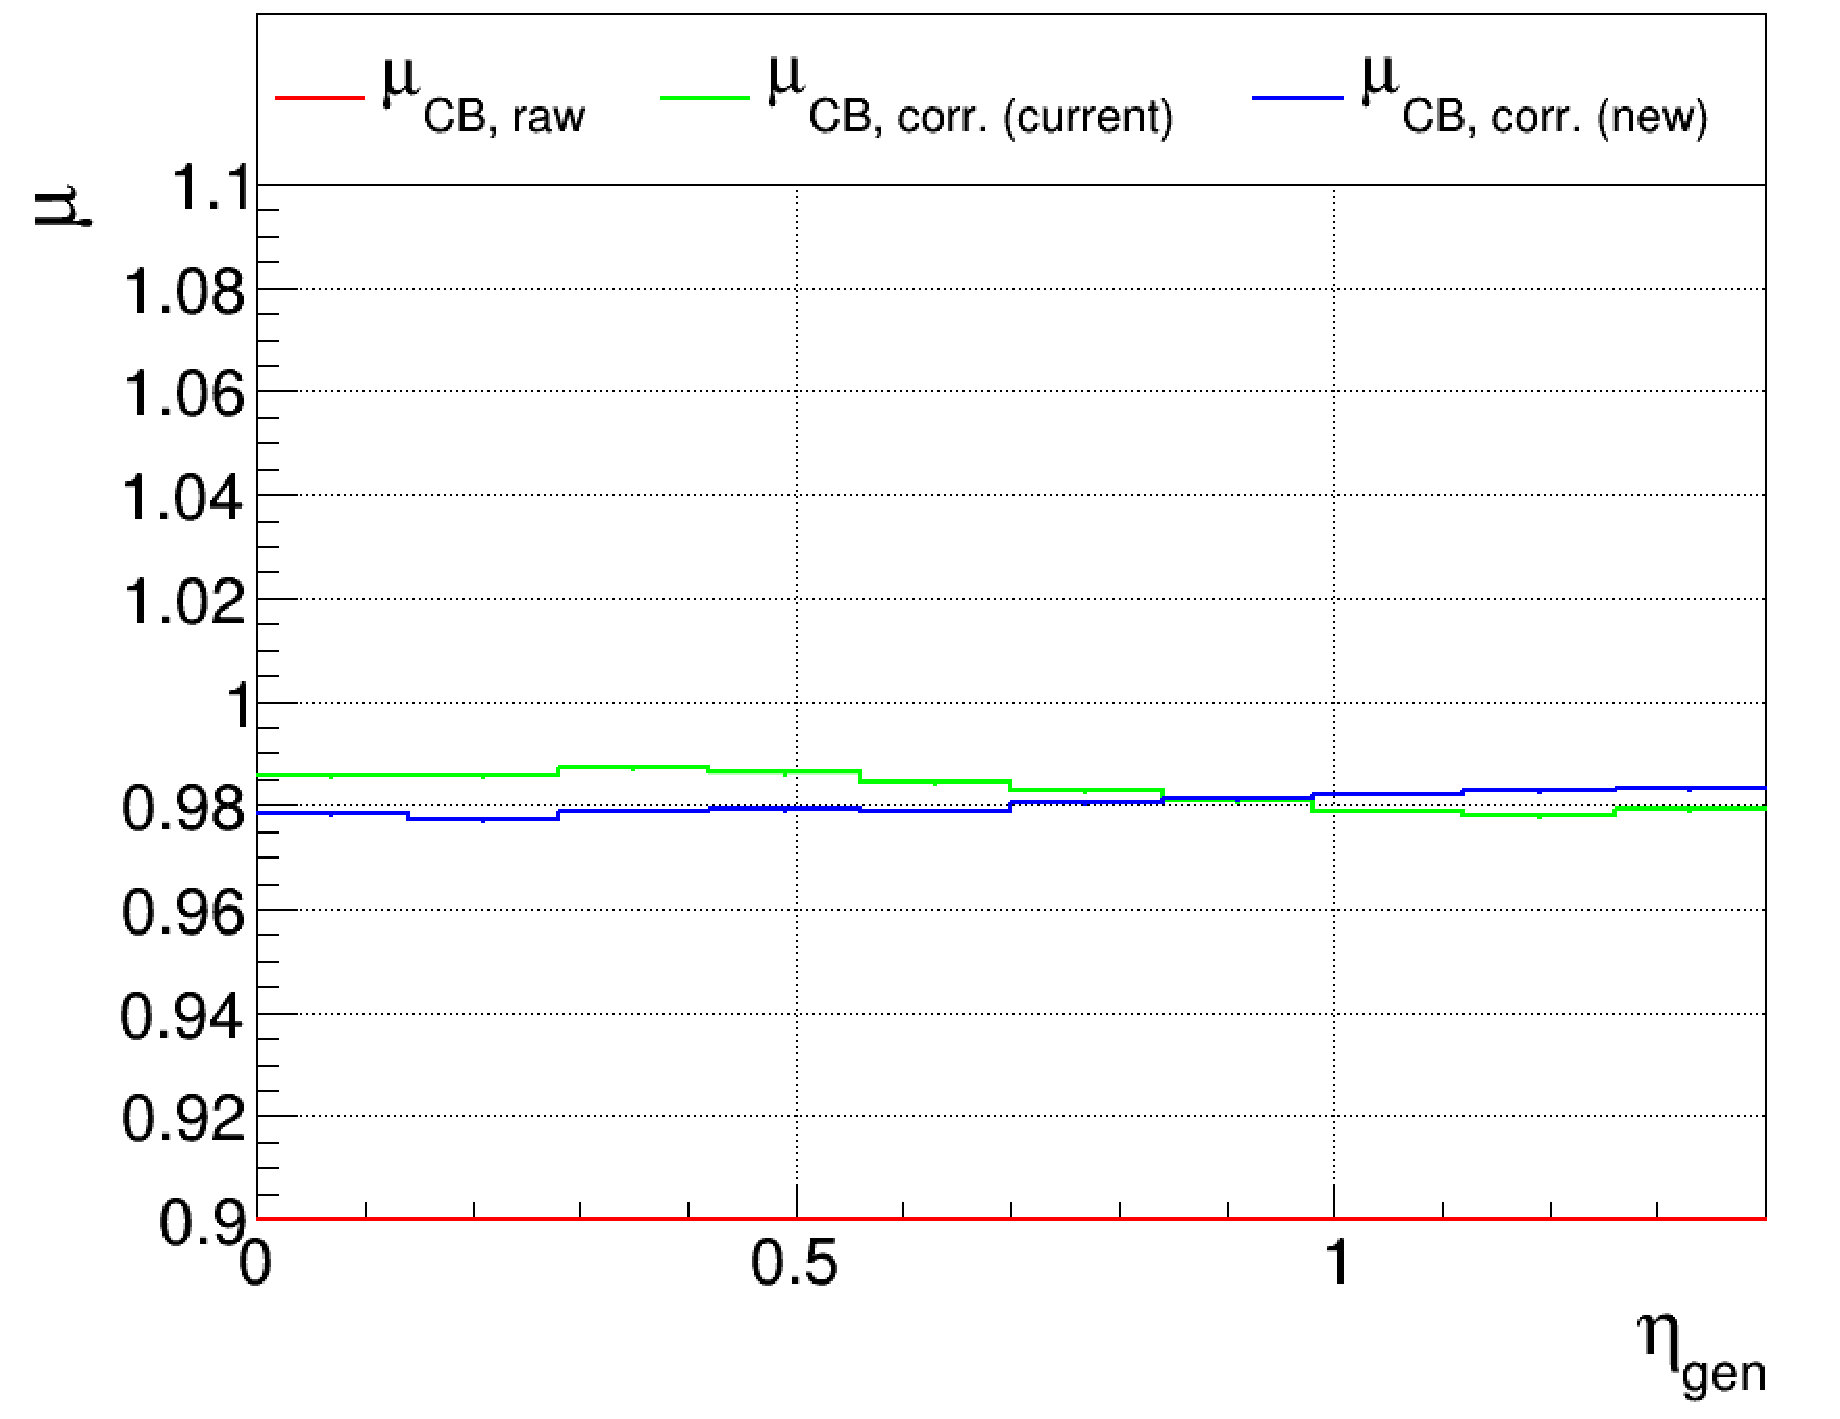
\includegraphics[width=0.495\textwidth]{./plots_pdf/ECAL_plots/plotsPU/EB/FULL/pdf/GENETA/EBFULL_GENETA_0005_0020_MuOverBins.pdf}
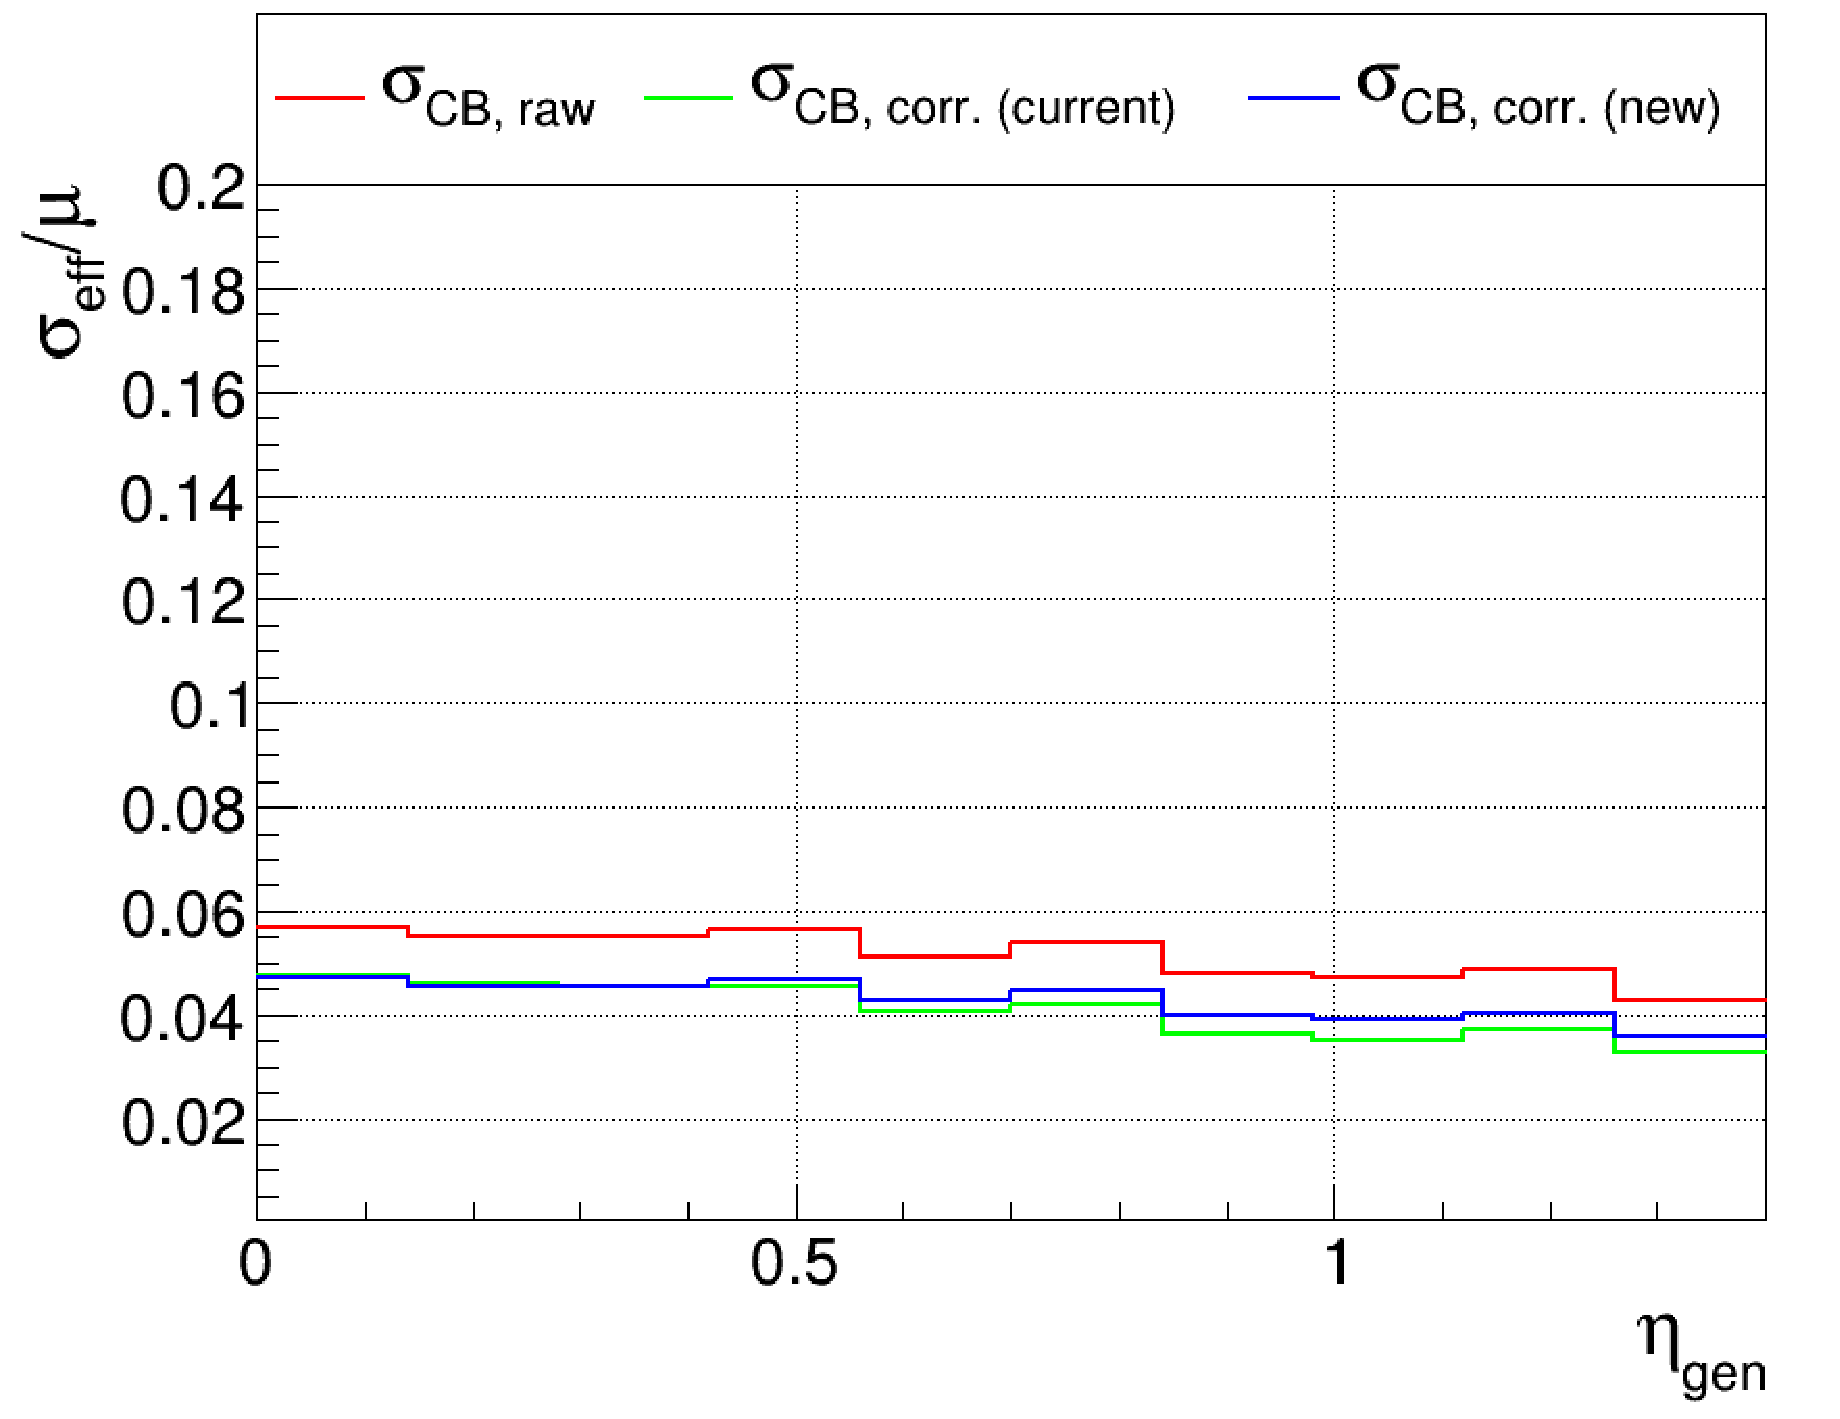
\includegraphics[width=0.495\textwidth]{./plots_pdf/ECAL_plots/plotsPU/EB/FULL/pdf/GENETA/EBFULL_GENETA_0005_0020_EffSigmaOverBins.pdf}
\caption{EB - Full Readout \pt 5--20\GeV.}
\end{figure}


\begin{figure}
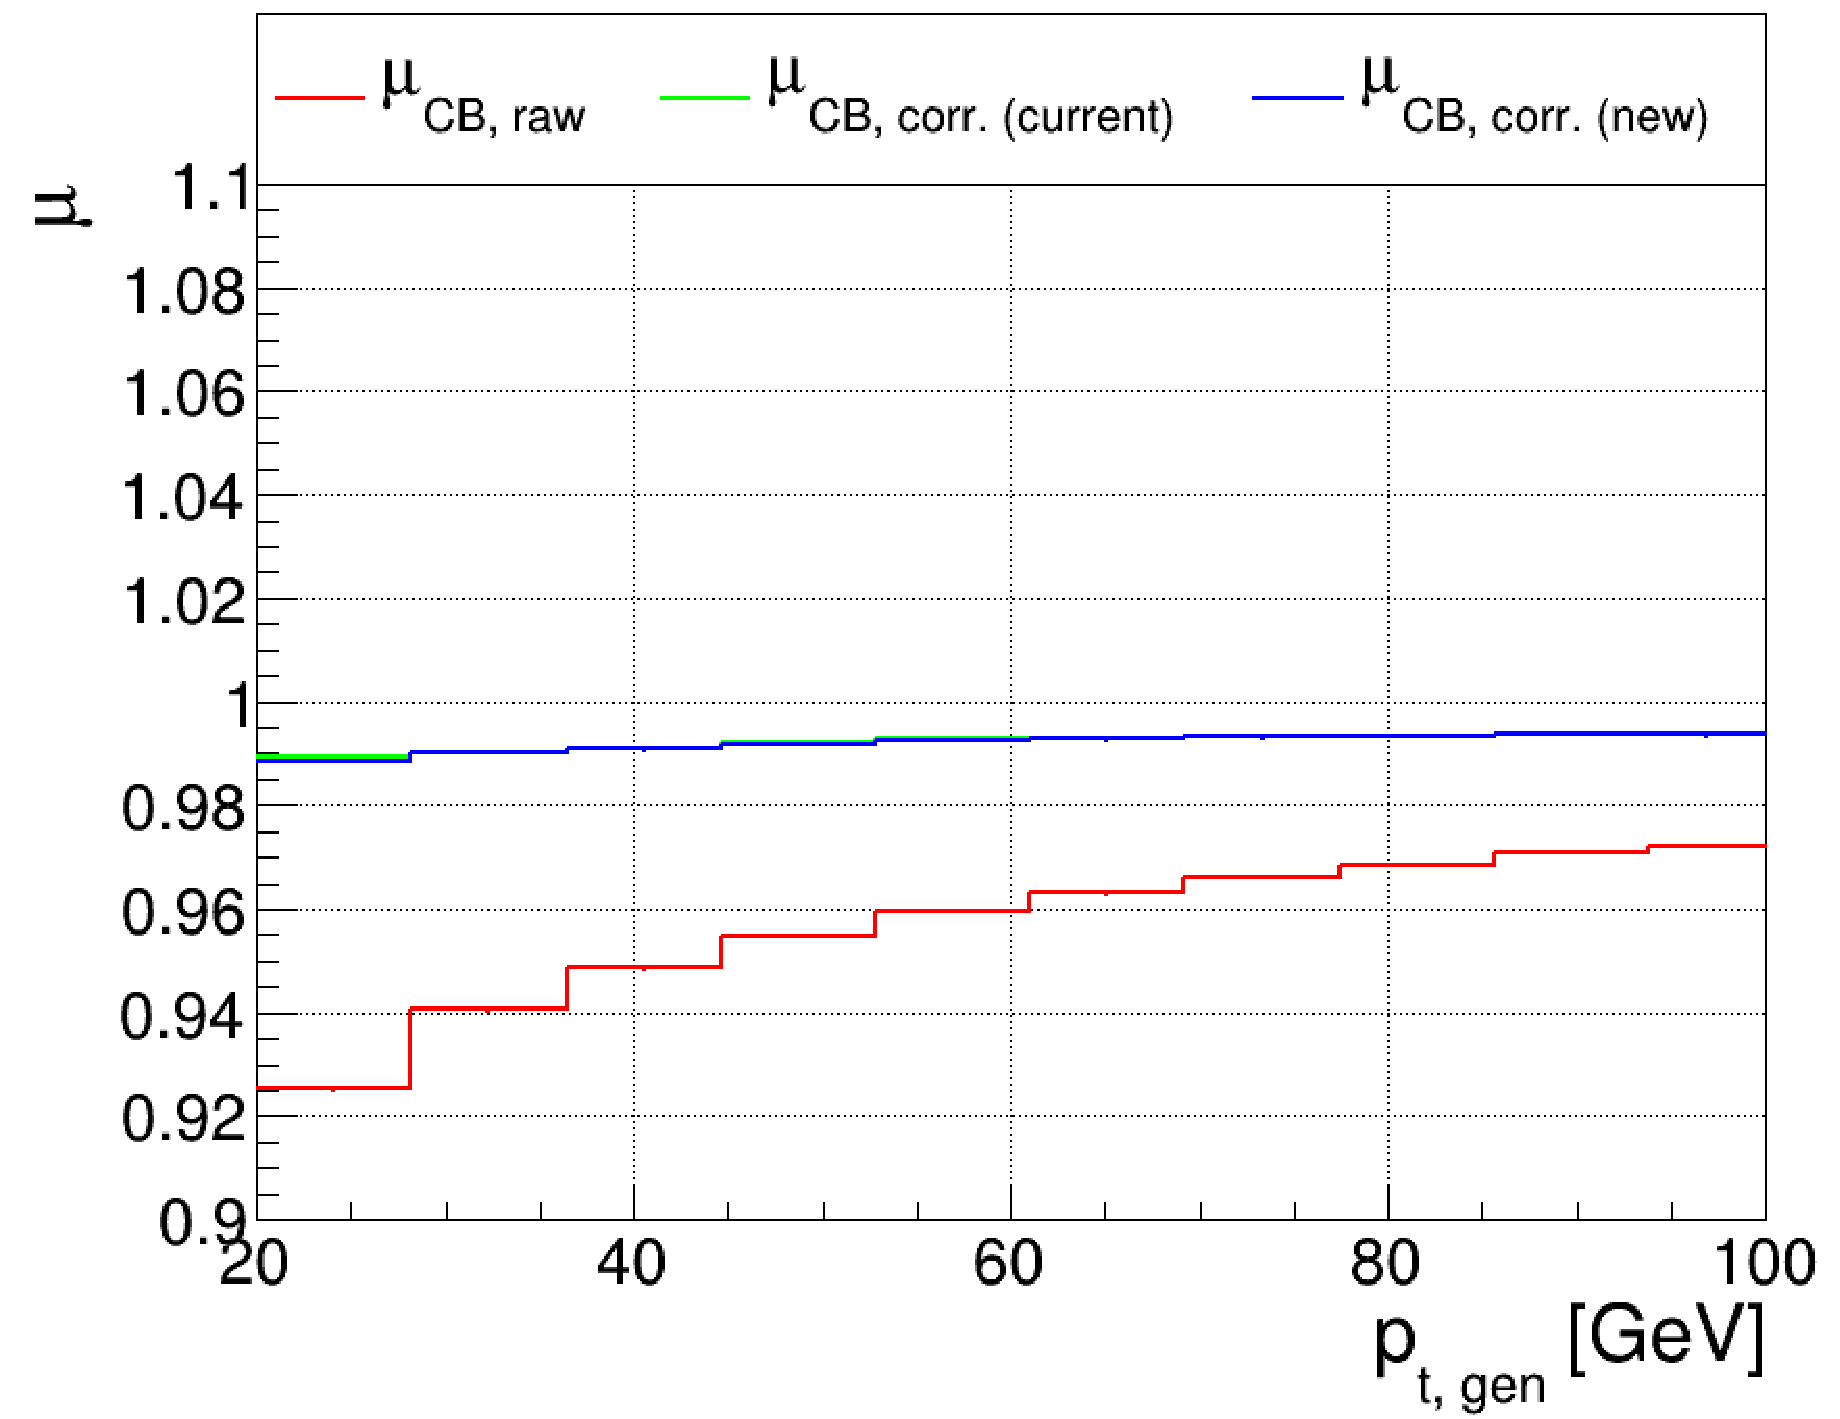
\includegraphics[width=0.495\textwidth]{./plots_pdf/ECAL_plots/plotsPU/EB/FULL/pdf/GENPT/EBFULL_GENPT_0020_0100_MuOverBins.pdf}
\includegraphics[width=0.495\textwidth]{./plots_pdf/ECAL_plots/plotsPU/EB/FULL/pdf/GENPT/EBFULL_GENPT_0020_0100_EffSigmaOverBins.pdf}
%\caption{EB - Full Readout pt 20-100}
%\end{figure}
%\begin{figure}
\includegraphics[width=0.495\textwidth]{./plots_pdf/ECAL_plots/plotsPU/EB/FULL/pdf/GENETA/EBFULL_GENETA_0020_0100_MuOverBins.pdf}
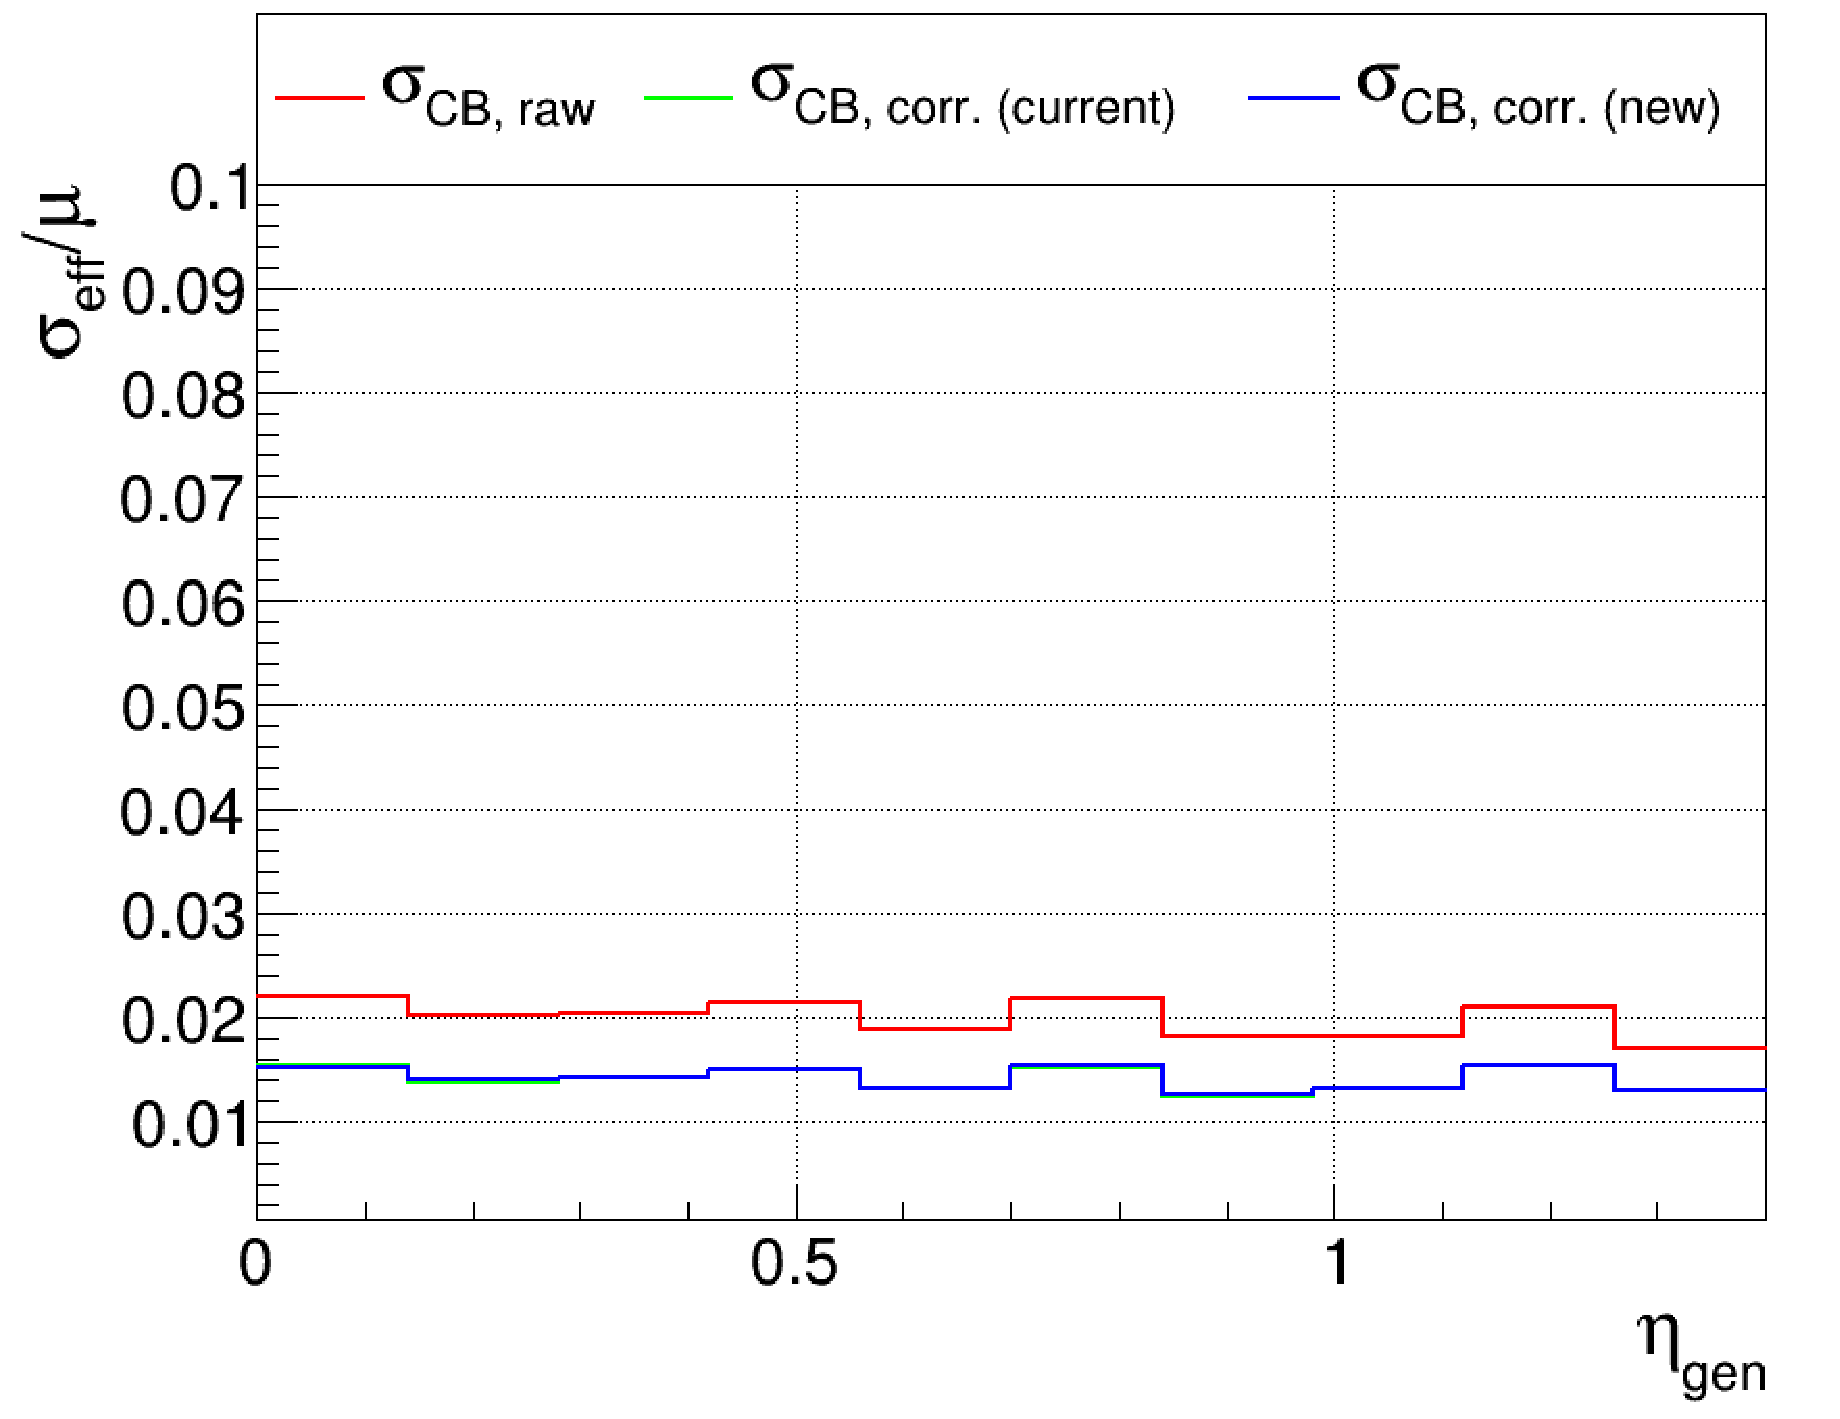
\includegraphics[width=0.495\textwidth]{./plots_pdf/ECAL_plots/plotsPU/EB/FULL/pdf/GENETA/EBFULL_GENETA_0020_0100_EffSigmaOverBins.pdf}
\caption{EB - Full Readout \pt 20--100\GeV.}
\end{figure}

\begin{figure}
\includegraphics[width=0.495\textwidth]{./plots_pdf/ECAL_plots/plotsPU/EB/FULL/pdf/GENPT/EBFULL_GENPT_0100_0300_MuOverBins.pdf}
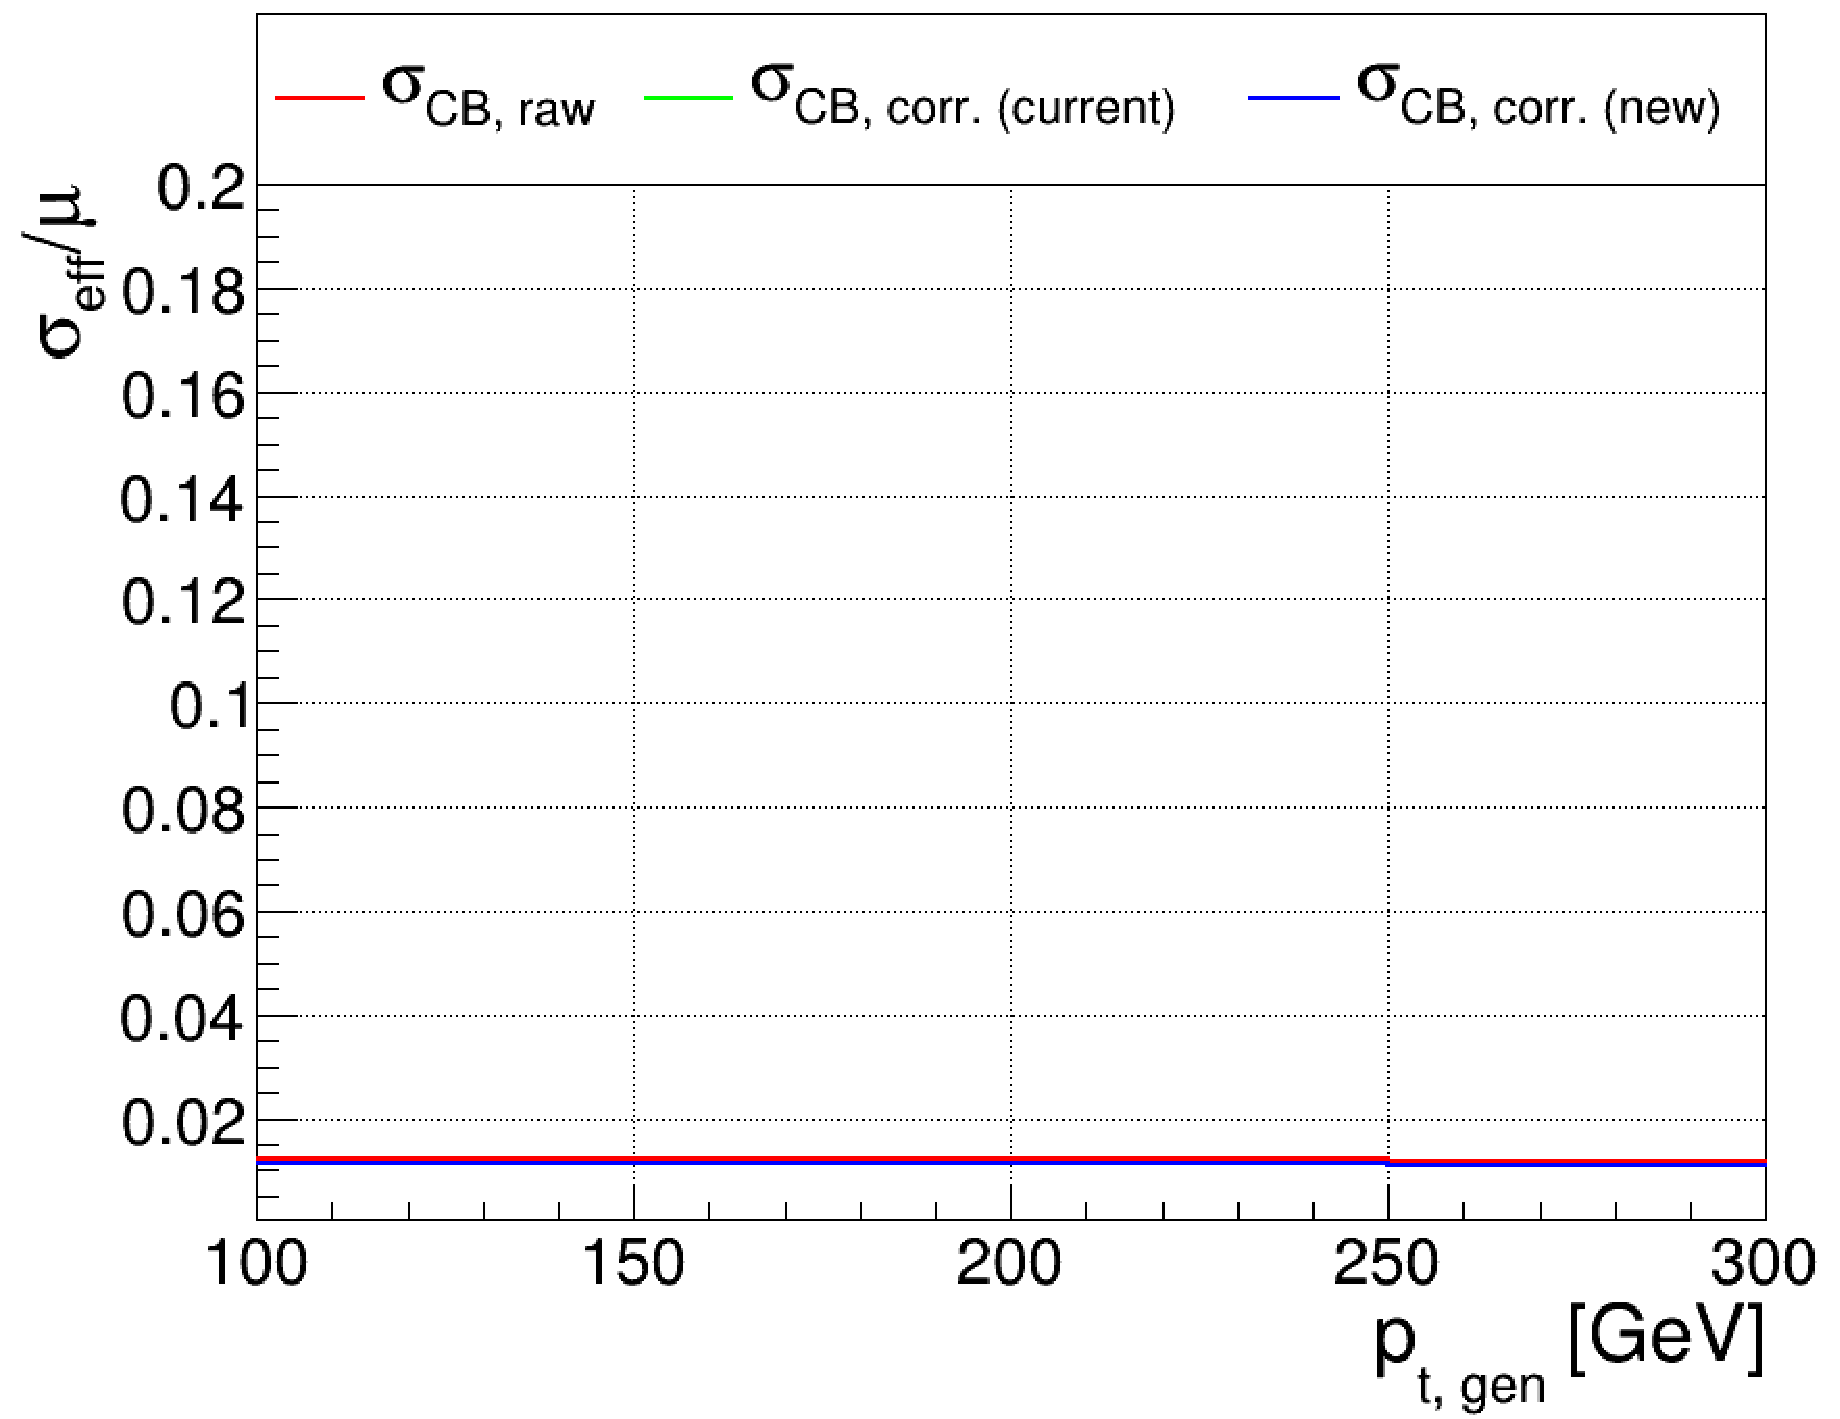
\includegraphics[width=0.495\textwidth]{./plots_pdf/ECAL_plots/plotsPU/EB/FULL/pdf/GENPT/EBFULL_GENPT_0100_0300_EffSigmaOverBins.pdf}
%\caption{EB - Full Readout pt 100-300}
%\end{figure}
%\begin{figure}
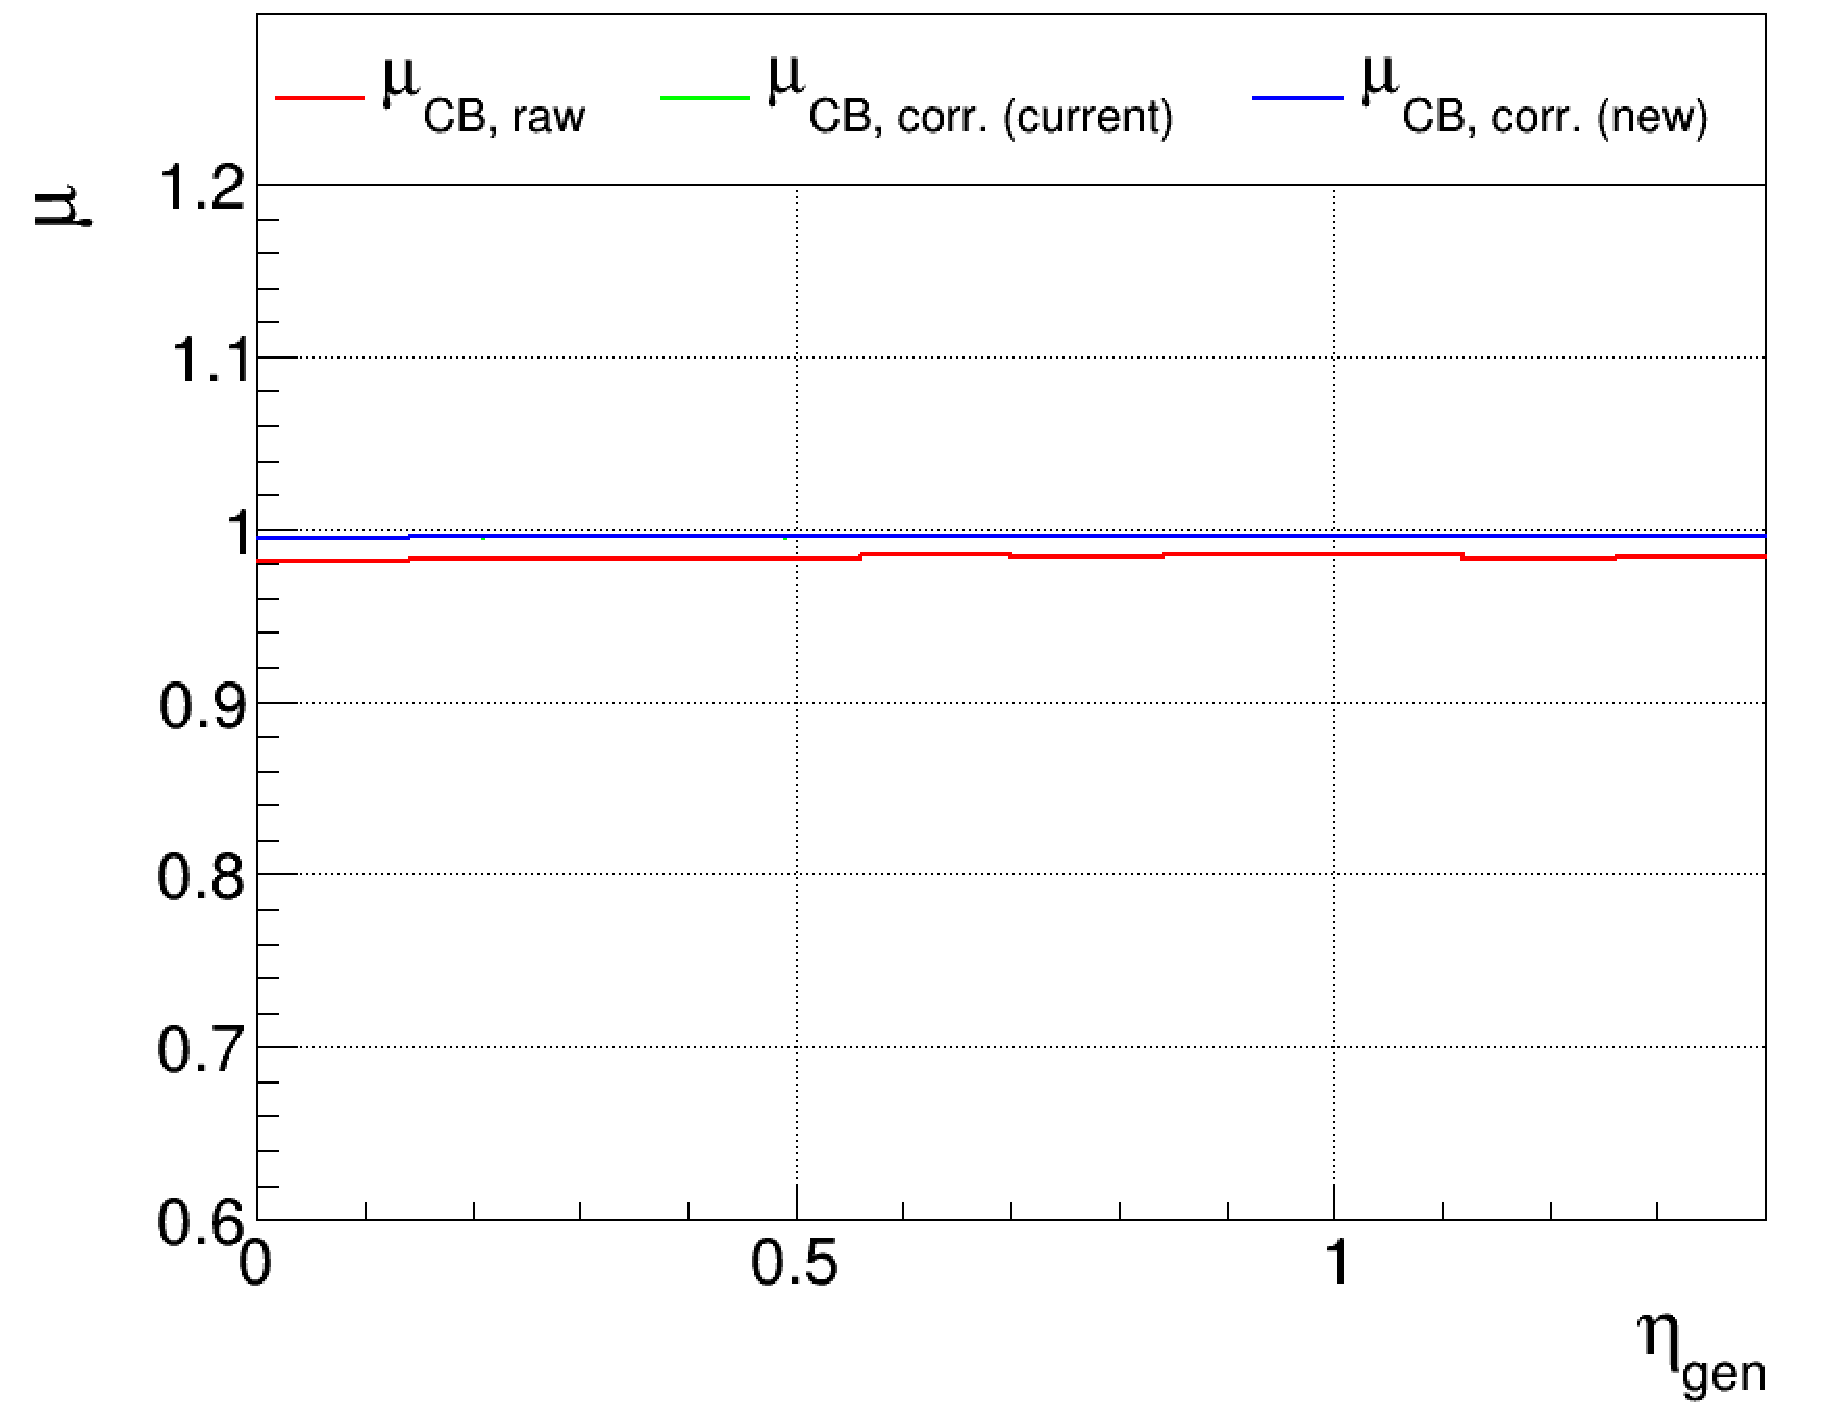
\includegraphics[width=0.495\textwidth]{./plots_pdf/ECAL_plots/plotsPU/EB/FULL/pdf/GENETA/EBFULL_GENETA_0100_0300_MuOverBins.pdf}
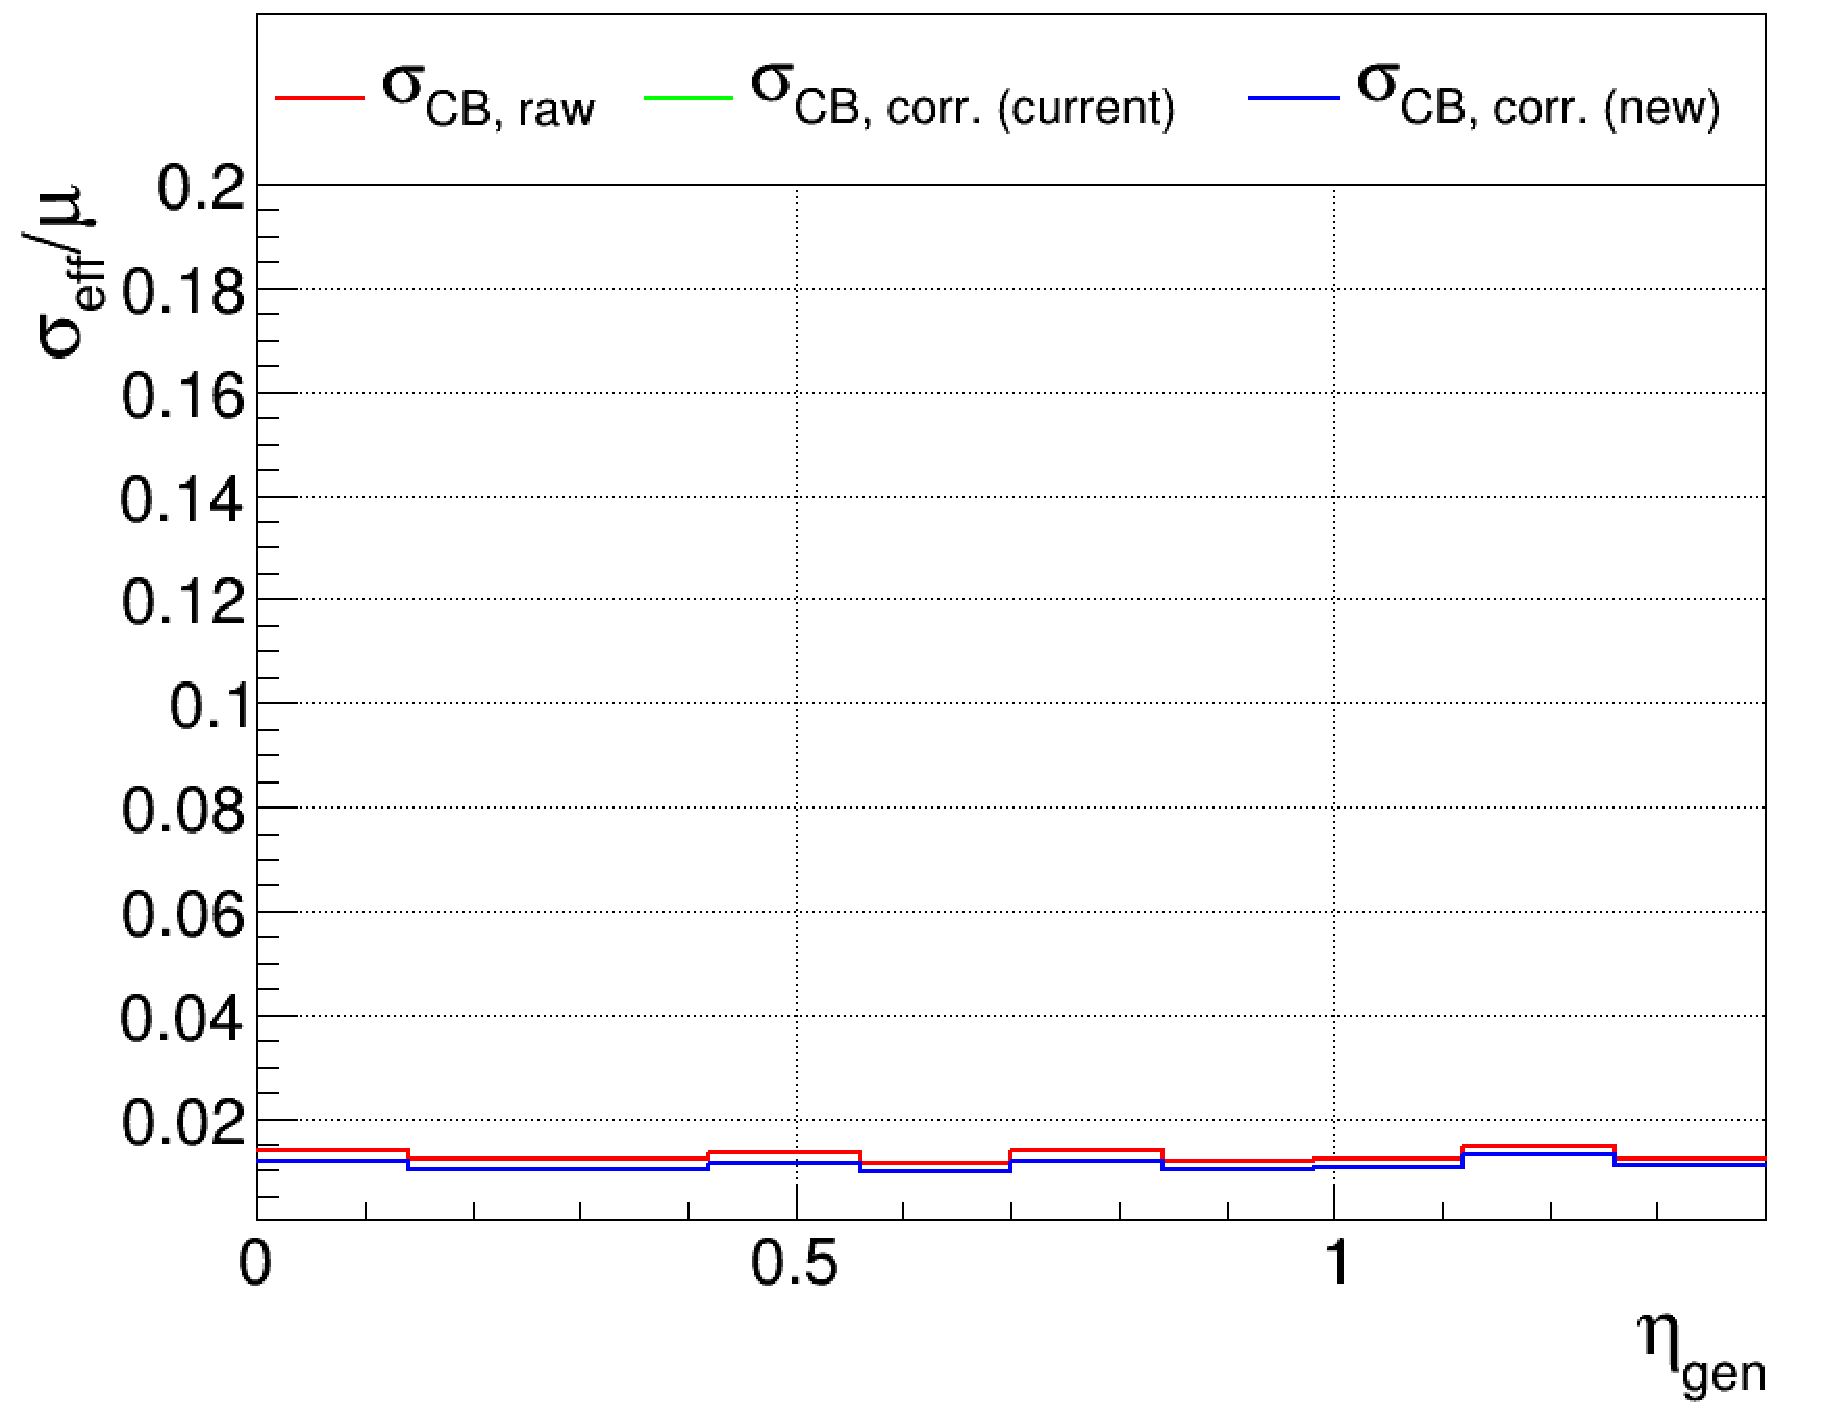
\includegraphics[width=0.495\textwidth]{./plots_pdf/ECAL_plots/plotsPU/EB/FULL/pdf/GENETA/EBFULL_GENETA_0100_0300_EffSigmaOverBins.pdf}
\caption{EB - Full Readout \pt 100-300\GeV}
\end{figure}





\begin{figure}
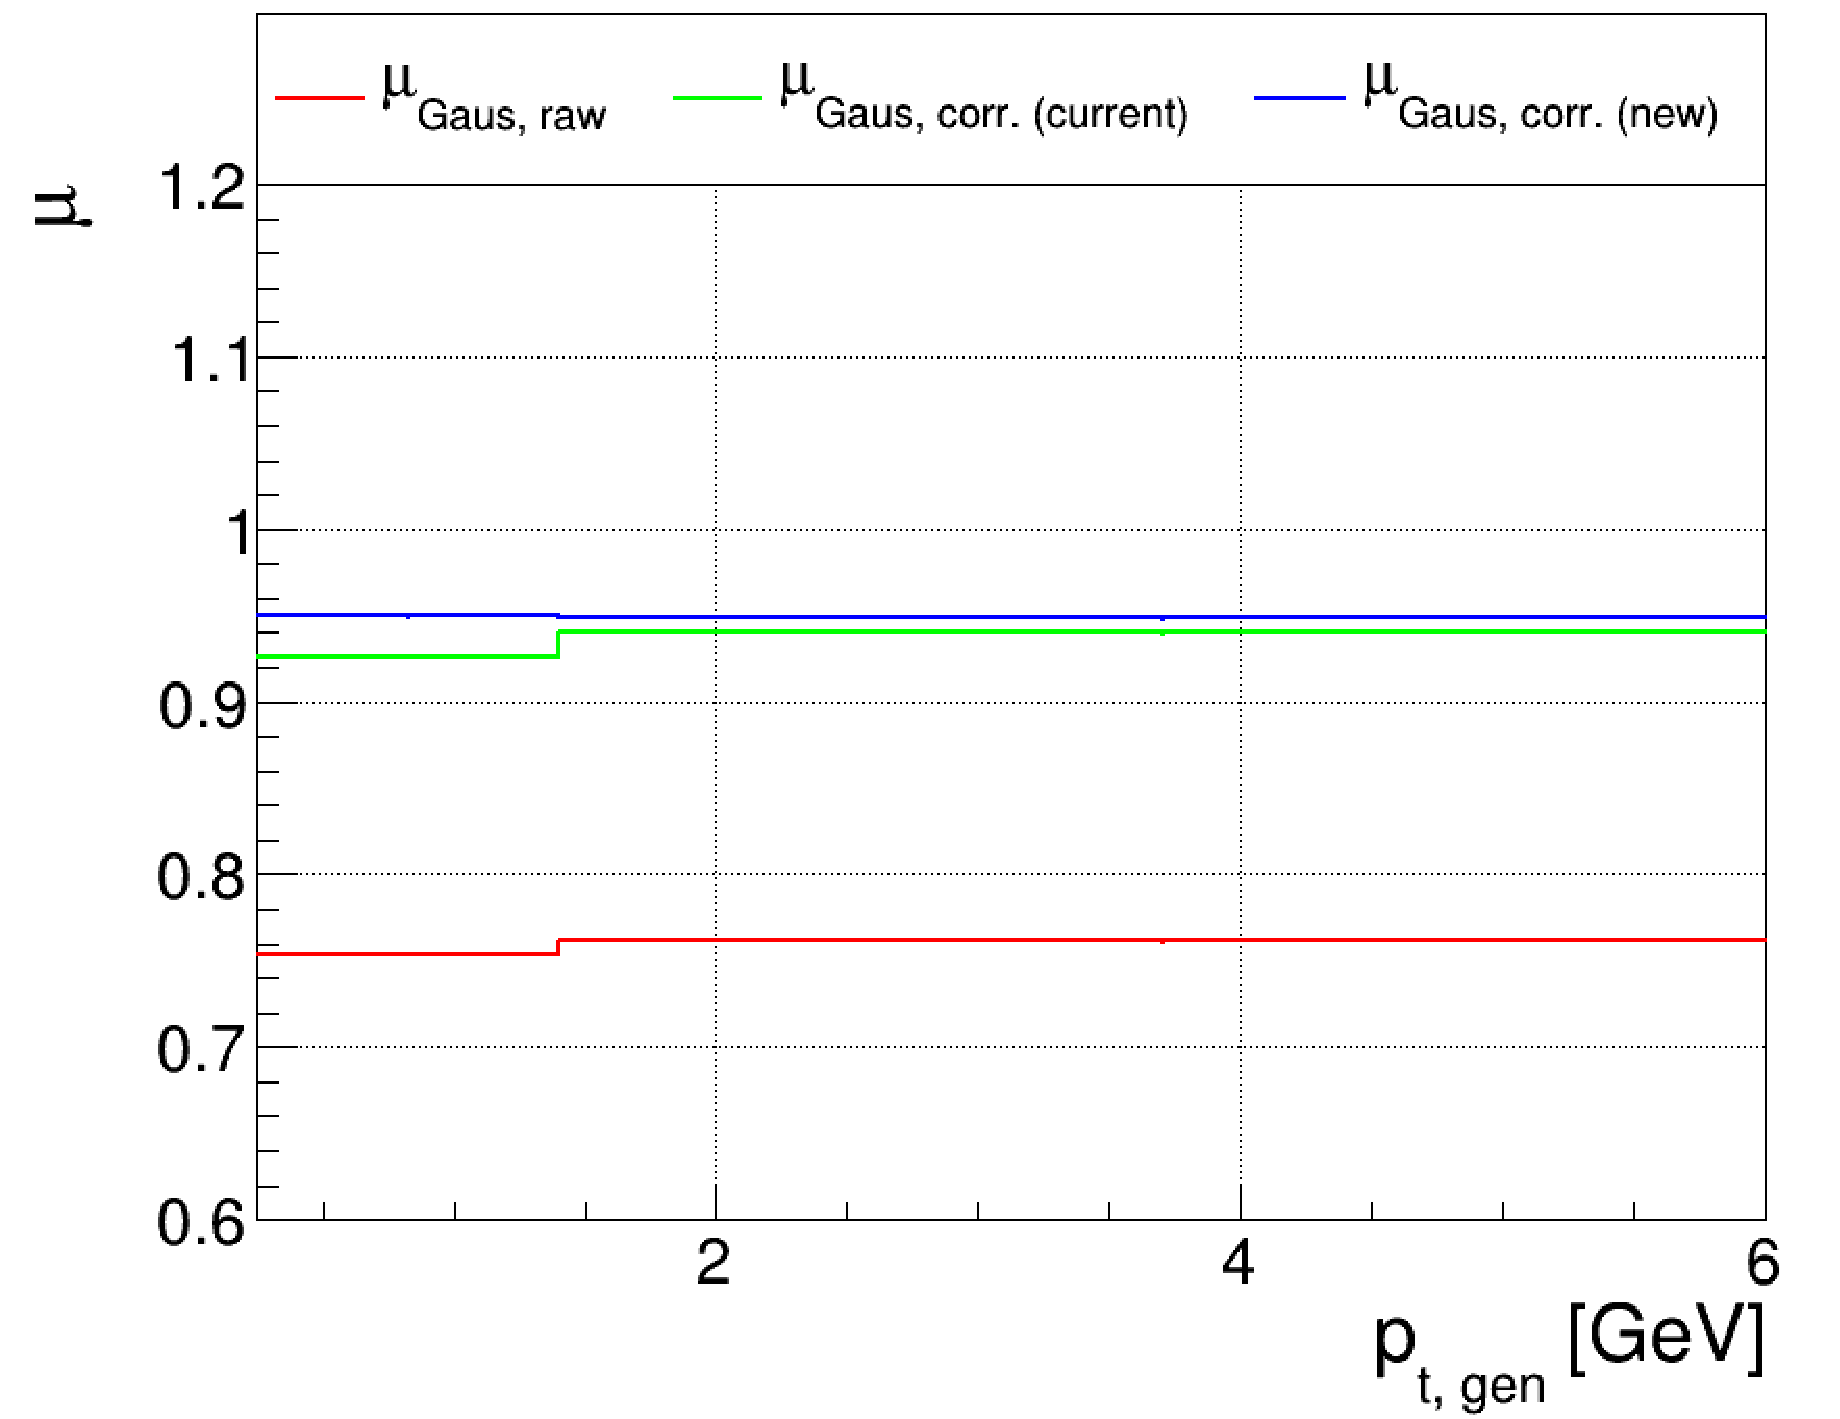
\includegraphics[width=0.495\textwidth]{./plots_pdf/ECAL_plots/plotsPU/EB/ZS/pdf/GENPT/EBZS_GENPT_0000_0006_MuOverBins.pdf}
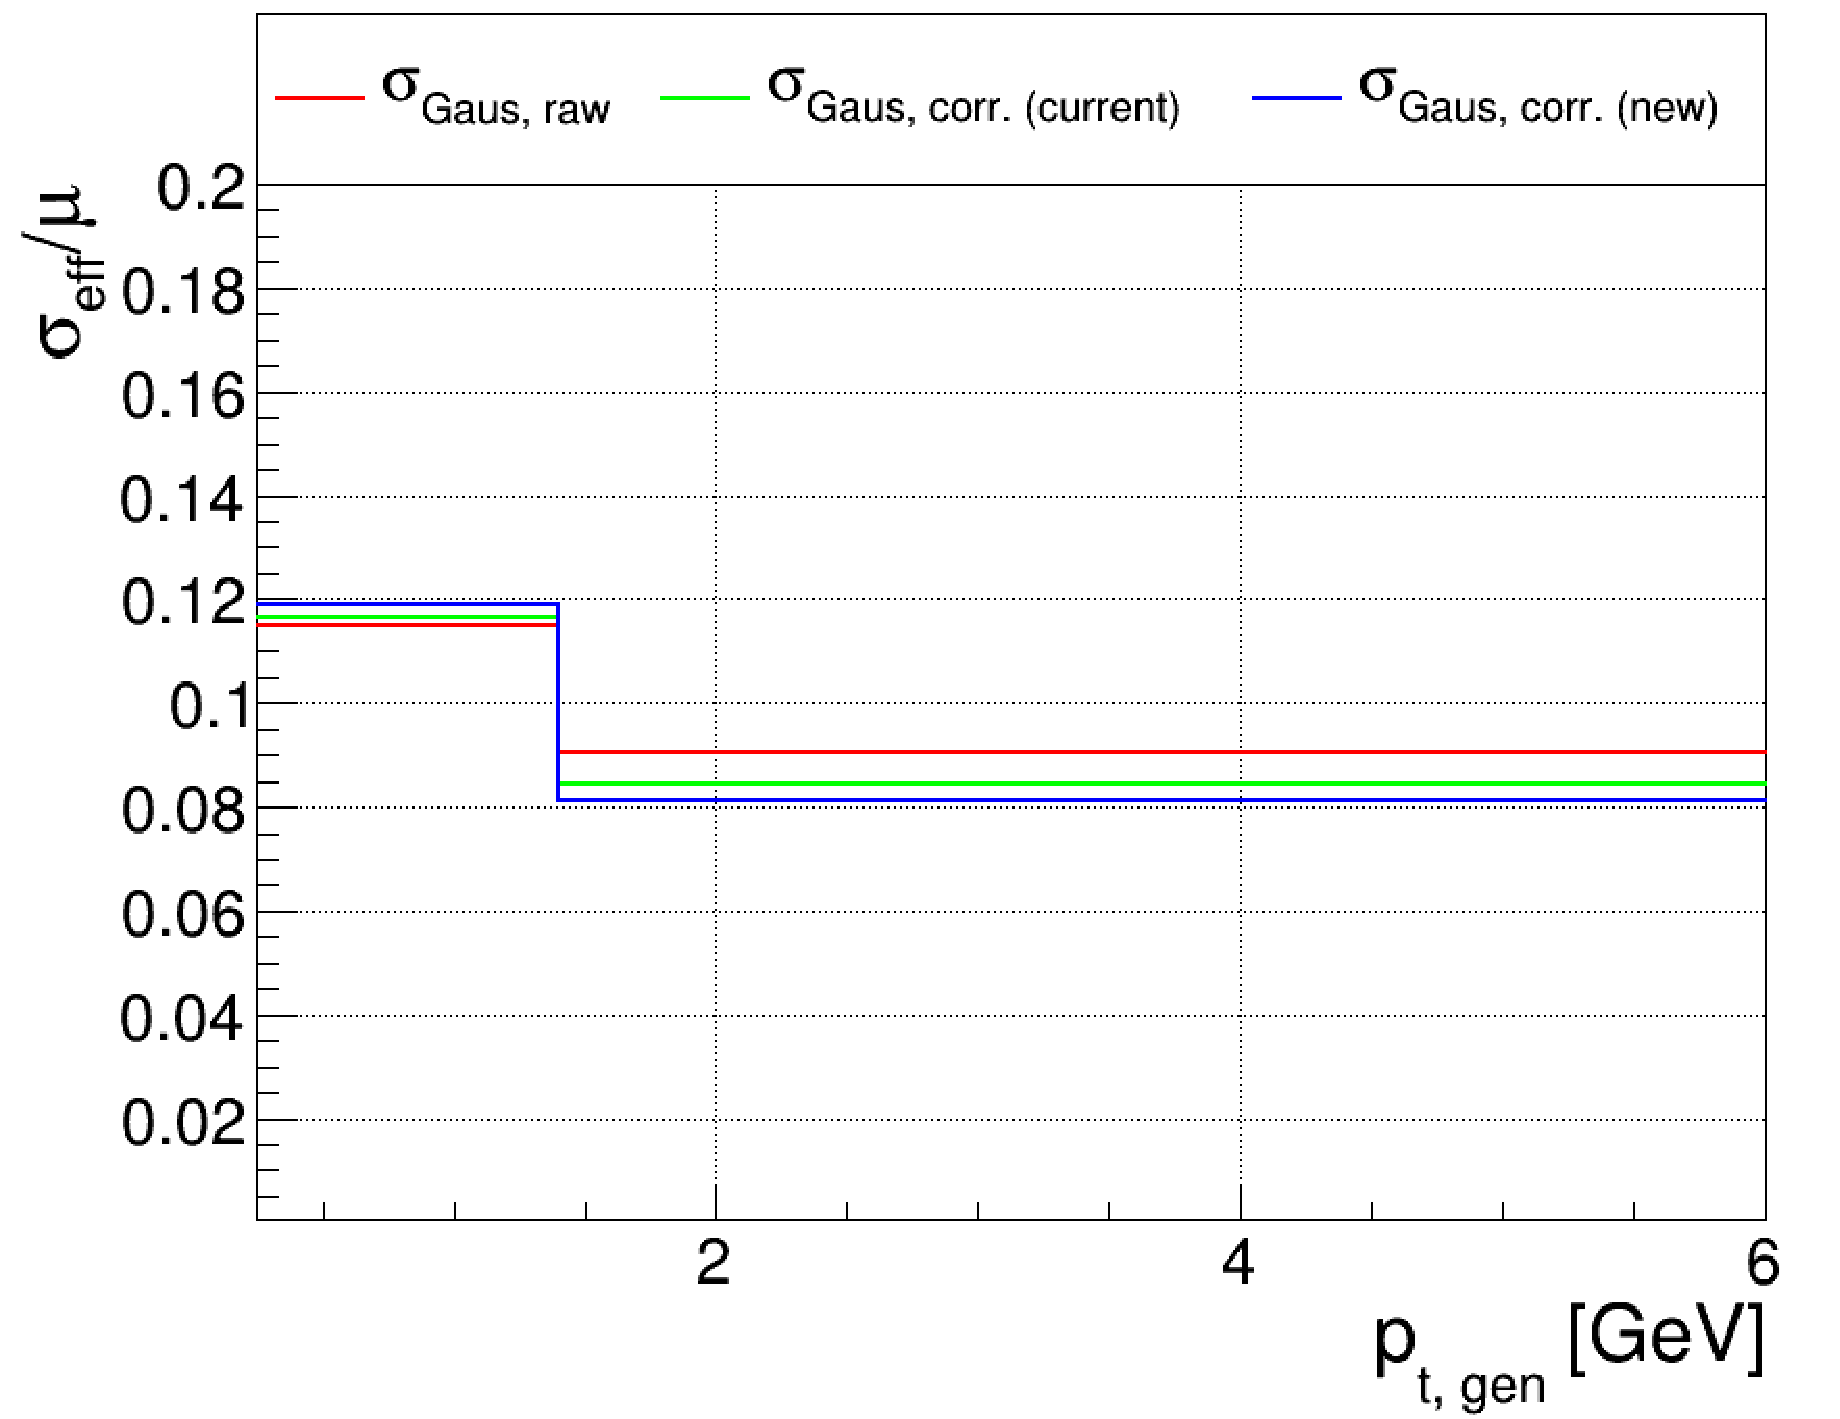
\includegraphics[width=0.495\textwidth]{./plots_pdf/ECAL_plots/plotsPU/EB/ZS/pdf/GENPT/EBZS_GENPT_0000_0006_EffSigmaOverBins.pdf}

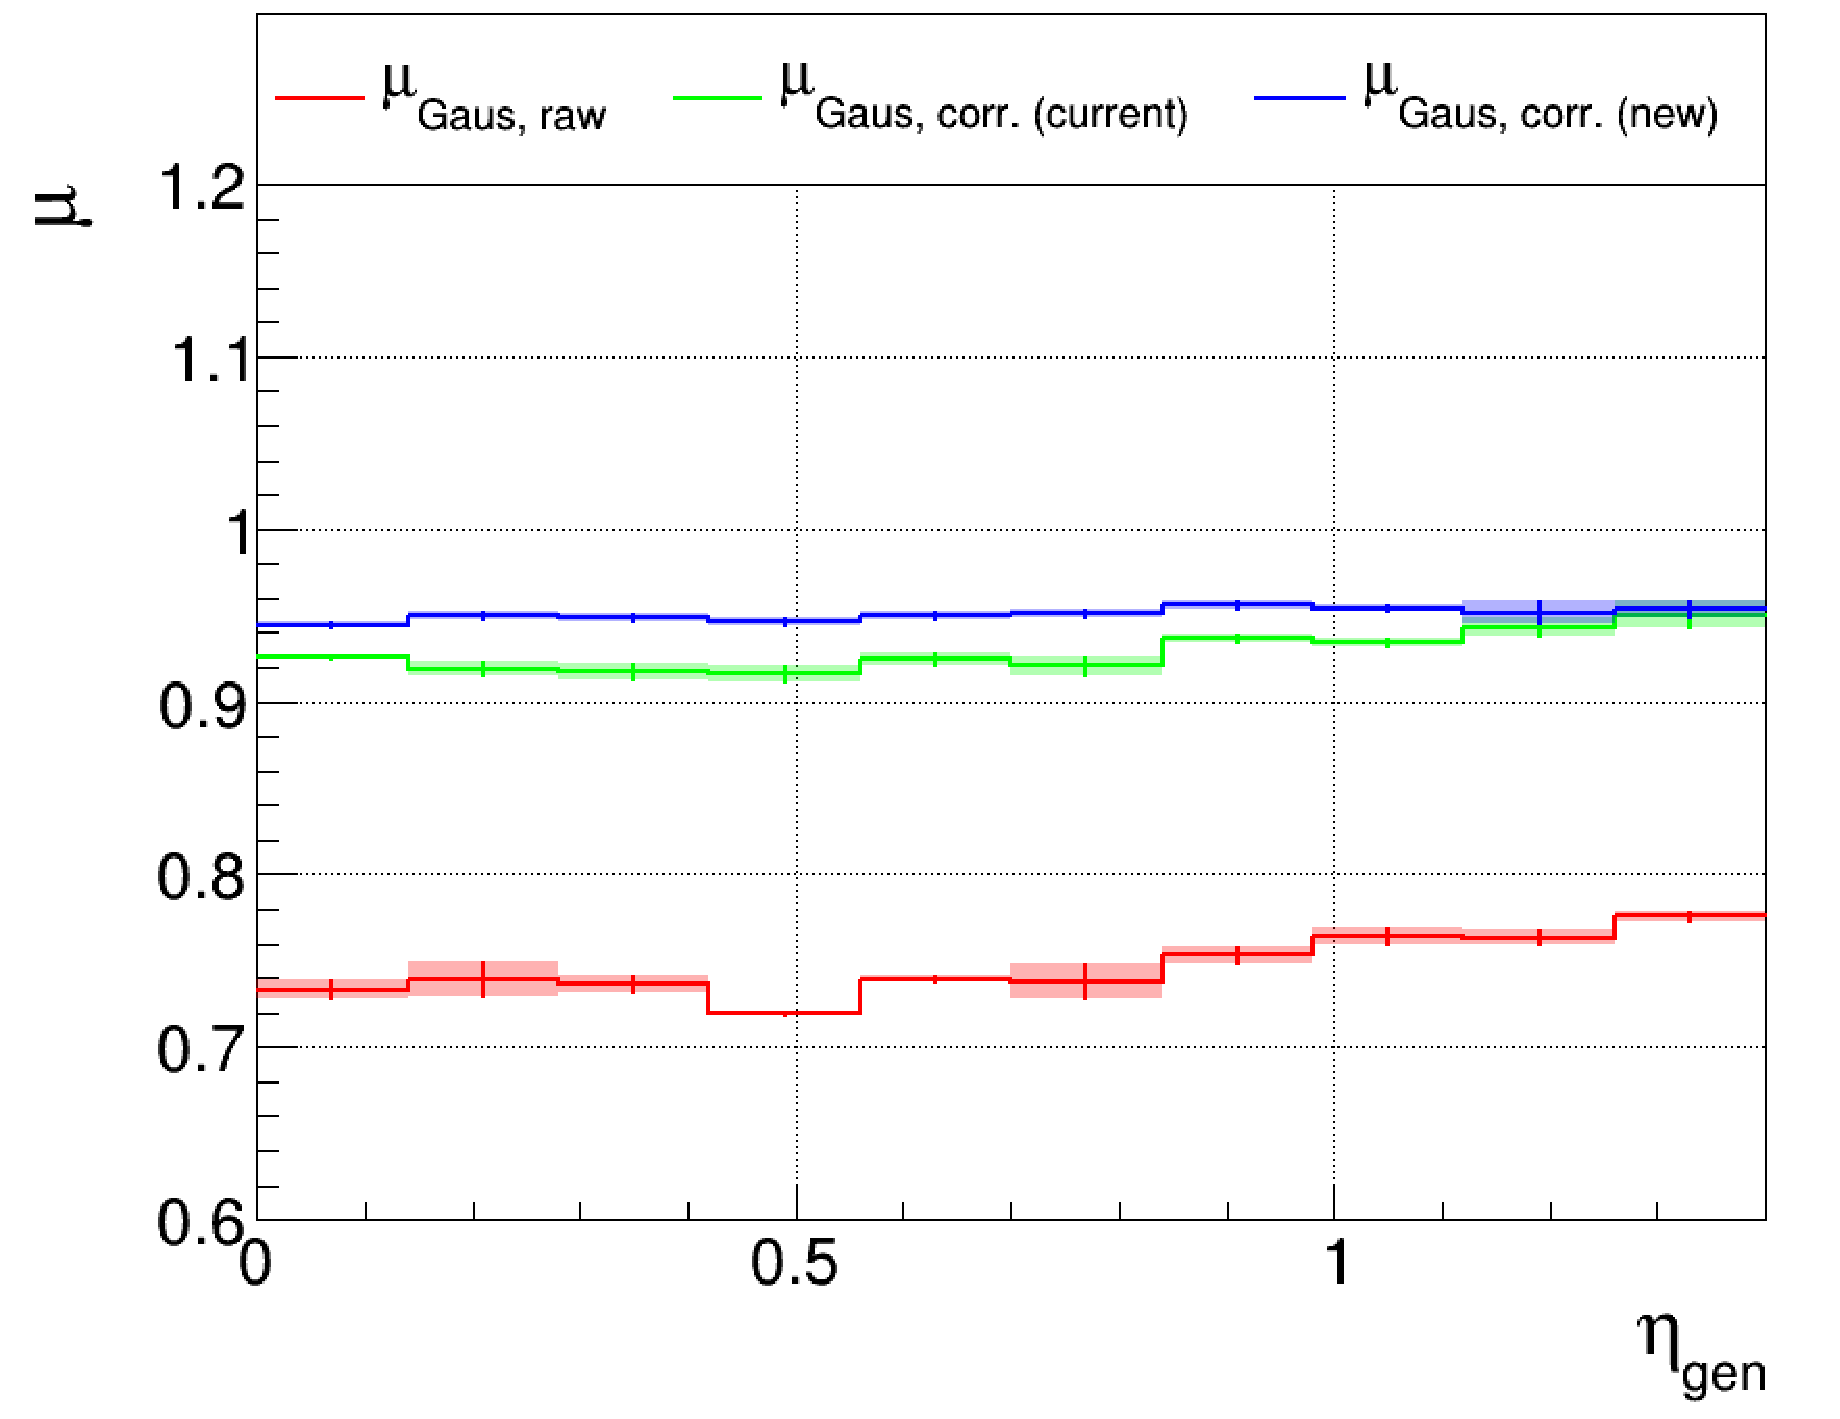
\includegraphics[width=0.495\textwidth]{./plots_pdf/ECAL_plots/plotsPU/EB/ZS/pdf/GENETA/EBZS_GENETA_0000_0006_MuOverBins.pdf}
\includegraphics[width=0.495\textwidth]{./plots_pdf/ECAL_plots/plotsPU/EB/ZS/pdf/GENETA/EBZS_GENETA_0000_0006_EffSigmaOverBins.pdf}
\caption[$\mu$ ($\sigma_\mathrm{eff}$) vs \pt of PF ECAL cluster - EB ZS readout PU  senario]{Mean response (resolution) defined by Raw PF ECAL clusters (red), the calibration derived earlier in Ru\
n3 based on 126X (green), and the new correction from 2024 simulation sample based on 133X (blue). \pt 0--6\GeV PU EB ZS readout PU senario.}
\label{fig:PU_EBZS}
\end{figure}

%% %\begin{figure}
%% \includegraphics[width=0.495\textwidth]{./plots_pdf/ECAL_plots/plotsPU/EB/ZS/pdf/GENPT/EBZS_GENPT_0006_0025_MuOverBins.pdf}
%% 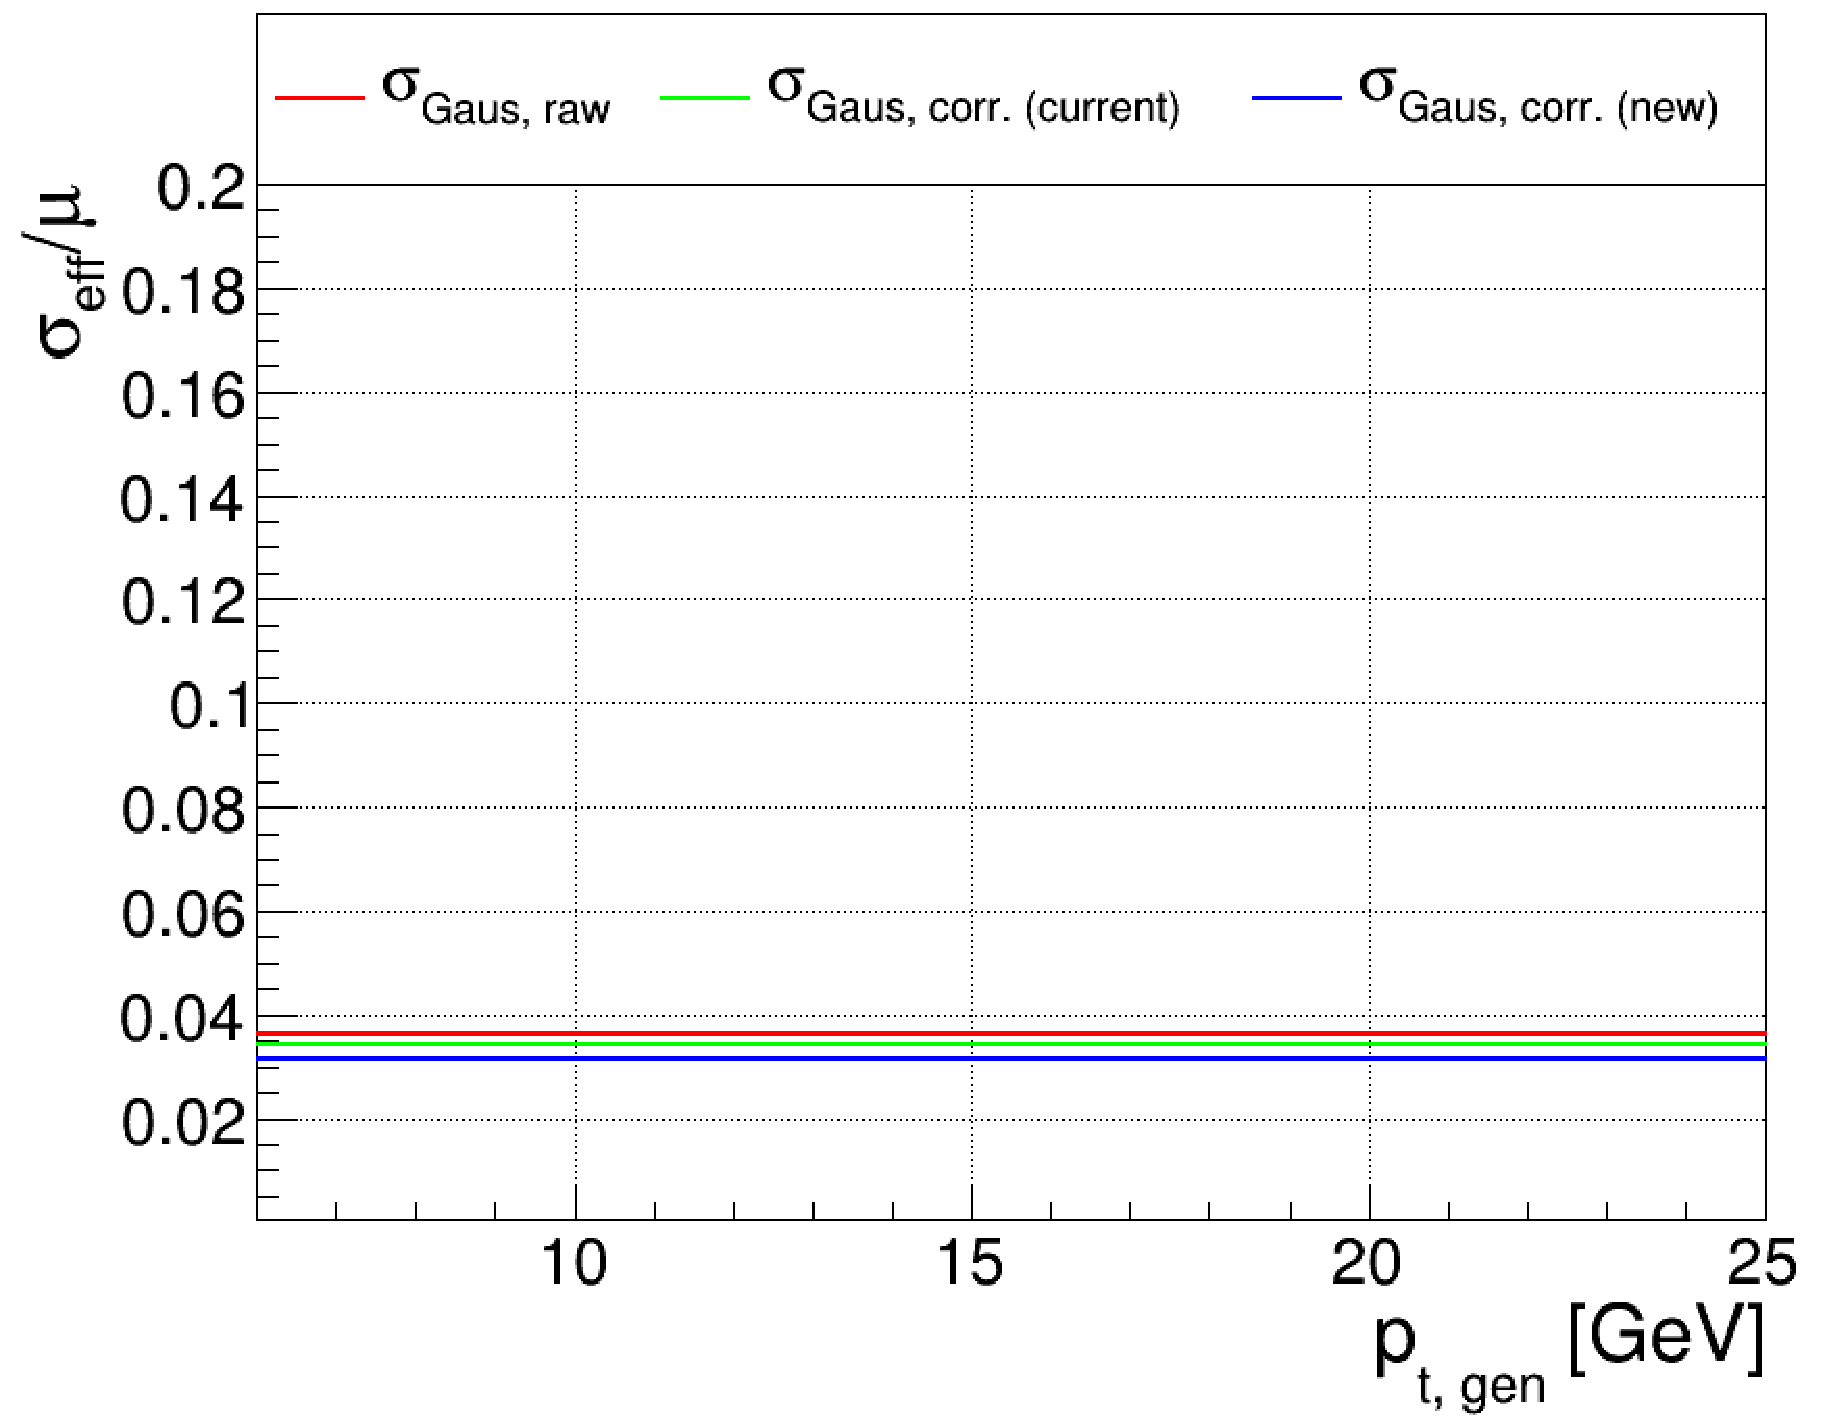
\includegraphics[width=0.495\textwidth]{./plots_pdf/ECAL_plots/plotsPU/EB/ZS/pdf/GENPT/EBZS_GENPT_0006_0025_EffSigmaOverBins.pdf}
%% %\caption{EB - ZS Readout pt 6-25}
%% %\end{figure}
%% %\begin{figure}
%% 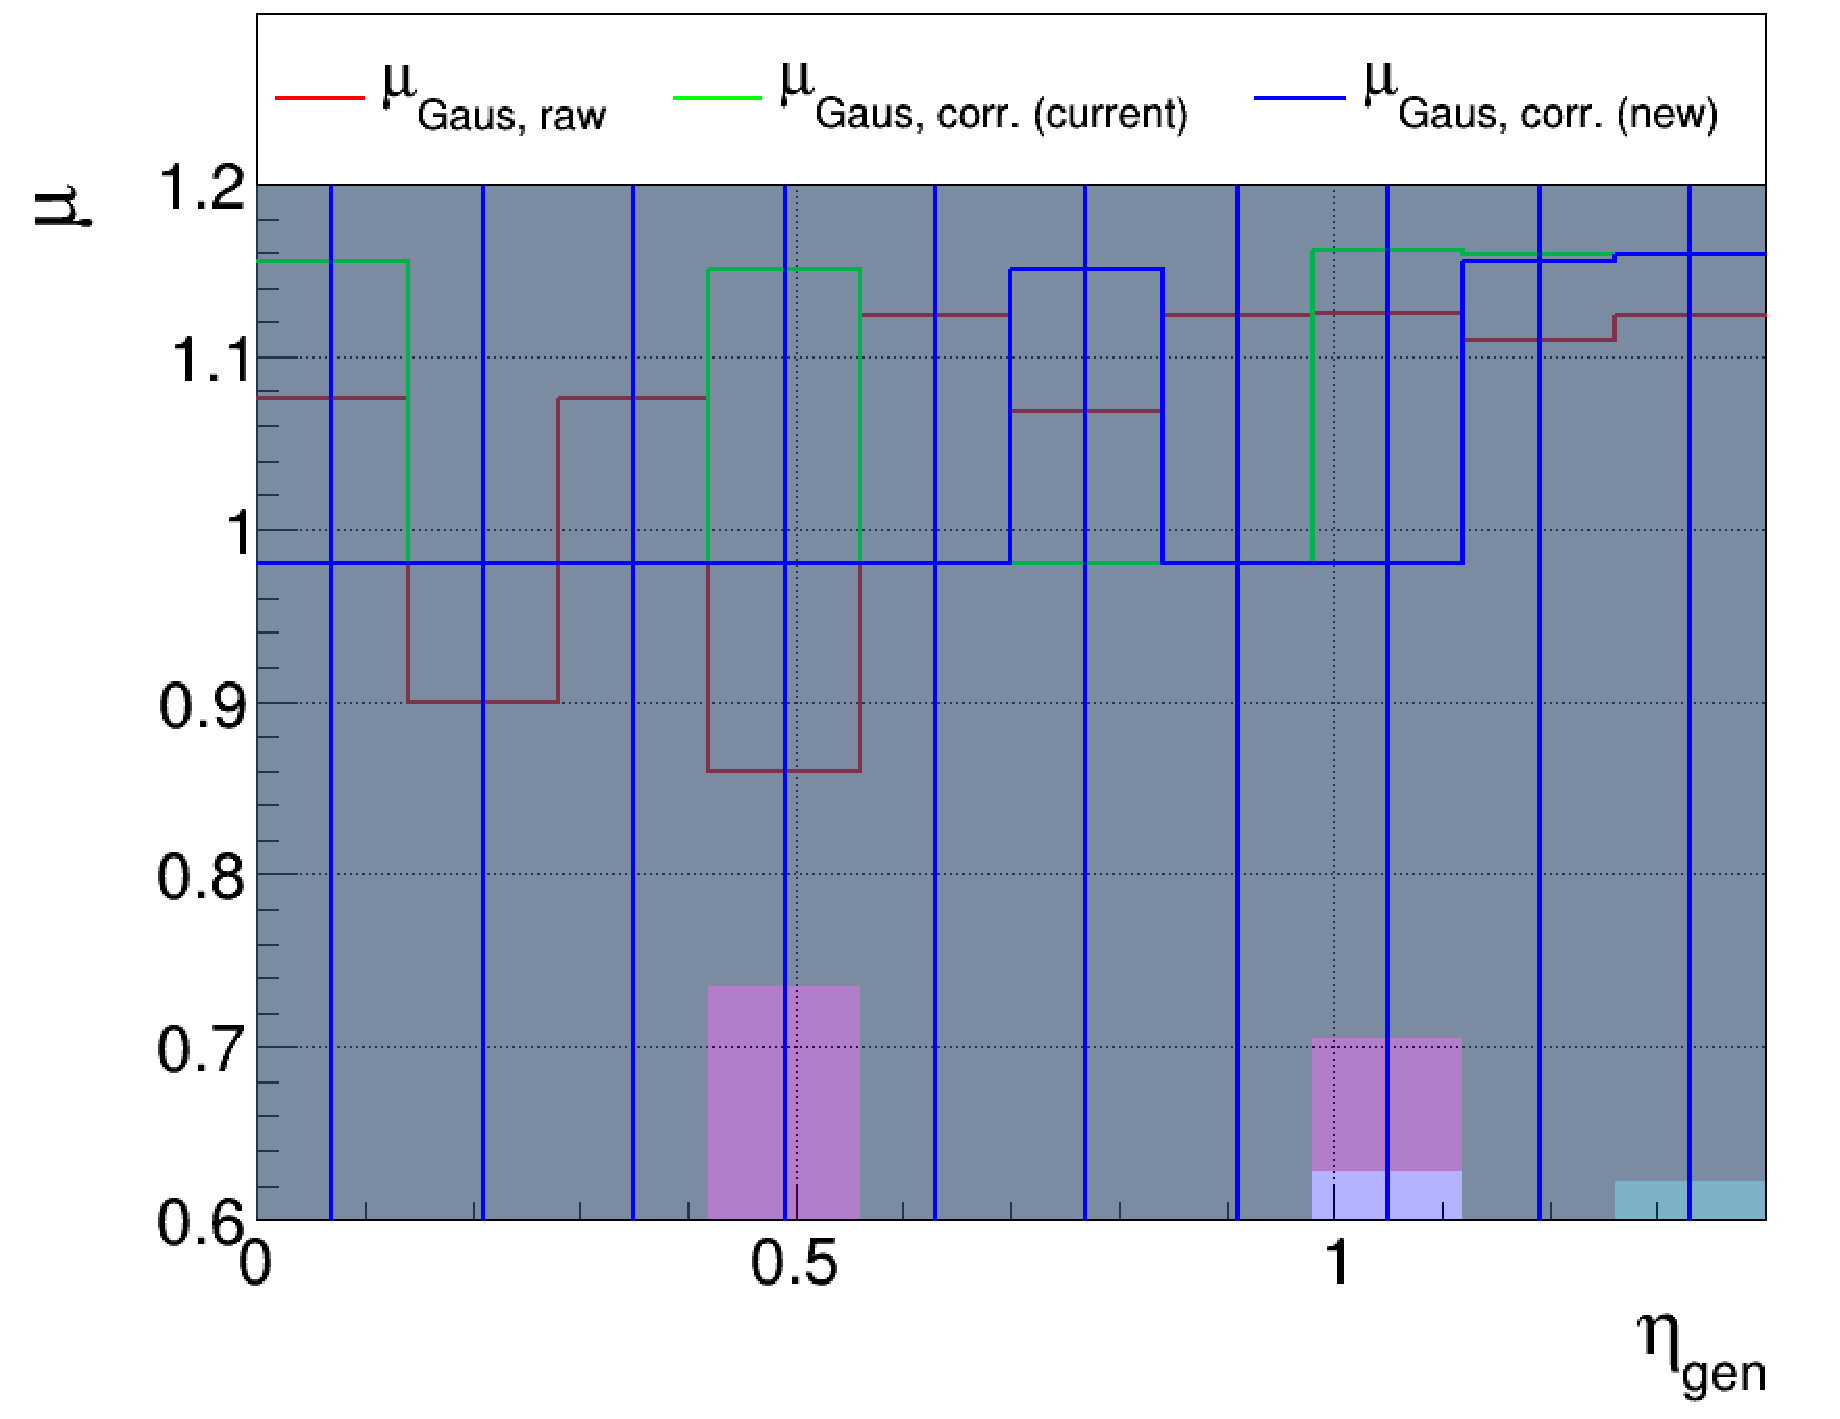
\includegraphics[width=0.495\textwidth]{./plots_pdf/ECAL_plots/plotsPU/EB/ZS/pdf/GENETA/EBZS_GENETA_0006_0025_MuOverBins.pdf}
%% 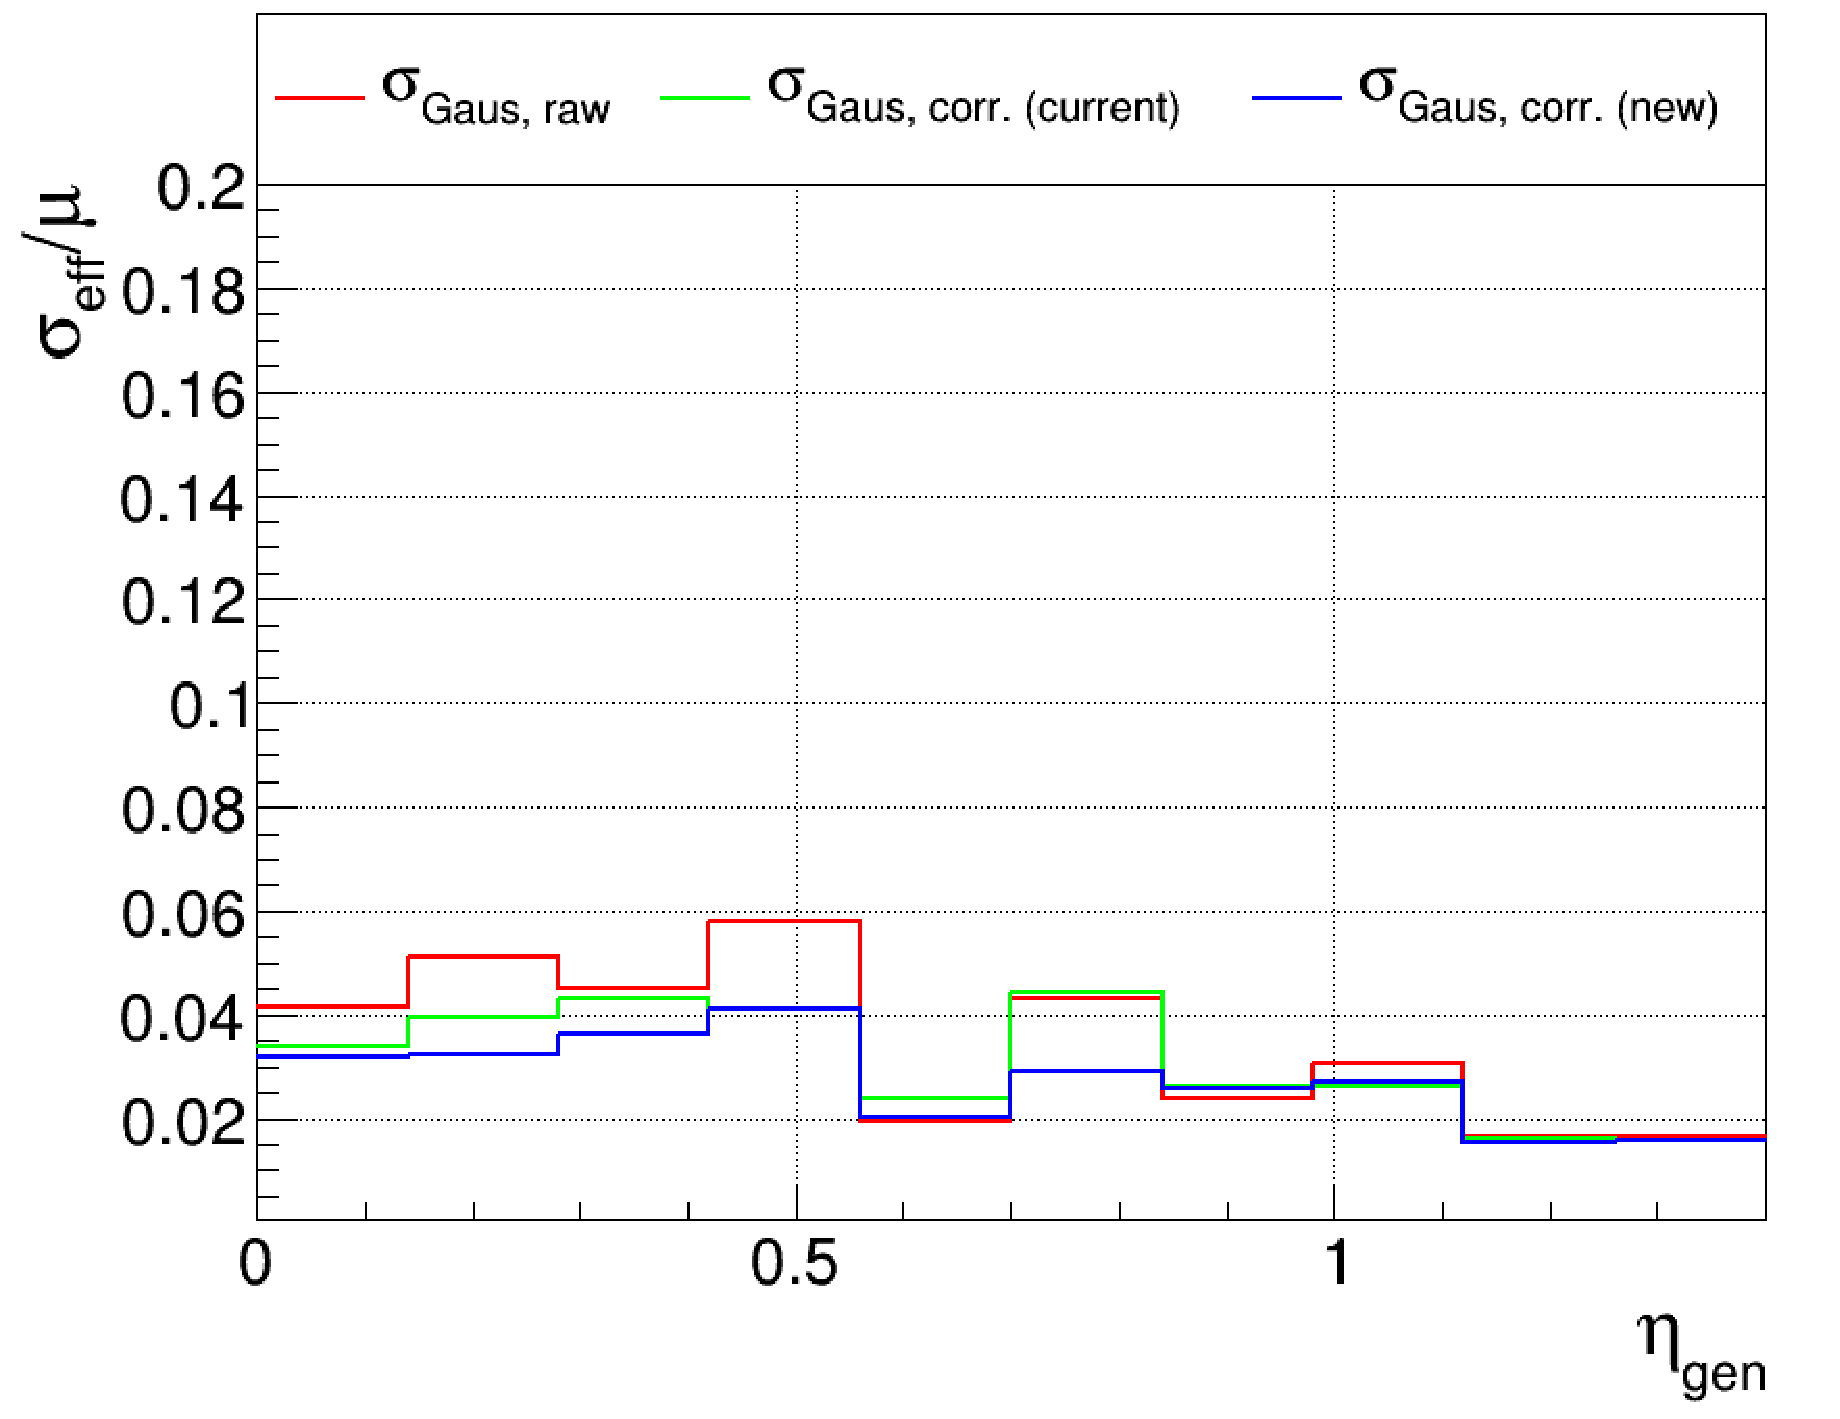
\includegraphics[width=0.495\textwidth]{./plots_pdf/ECAL_plots/plotsPU/EB/ZS/pdf/GENETA/EBZS_GENETA_0006_0025_EffSigmaOverBins.pdf}
%% \caption{EB - ZS Readout \pt 6-25}
%% \end{figure}







\begin{figure}
  %5-20 pt 
\includegraphics[width=0.335\textwidth]{./plots_pdf/ECAL_plots/plotsNOPU/EB/FULL/pdf/GENPT/EBFULL_GENPT_0005_0020_MuOverBins.pdf}
\includegraphics[width=0.3355\textwidth]{./plots_pdf/ECAL_plots/plotsNOPU/EB/FULL/pdf/GENPT/EBFULL_GENPT_0005_0020_EffSigmaOverBins.pdf}

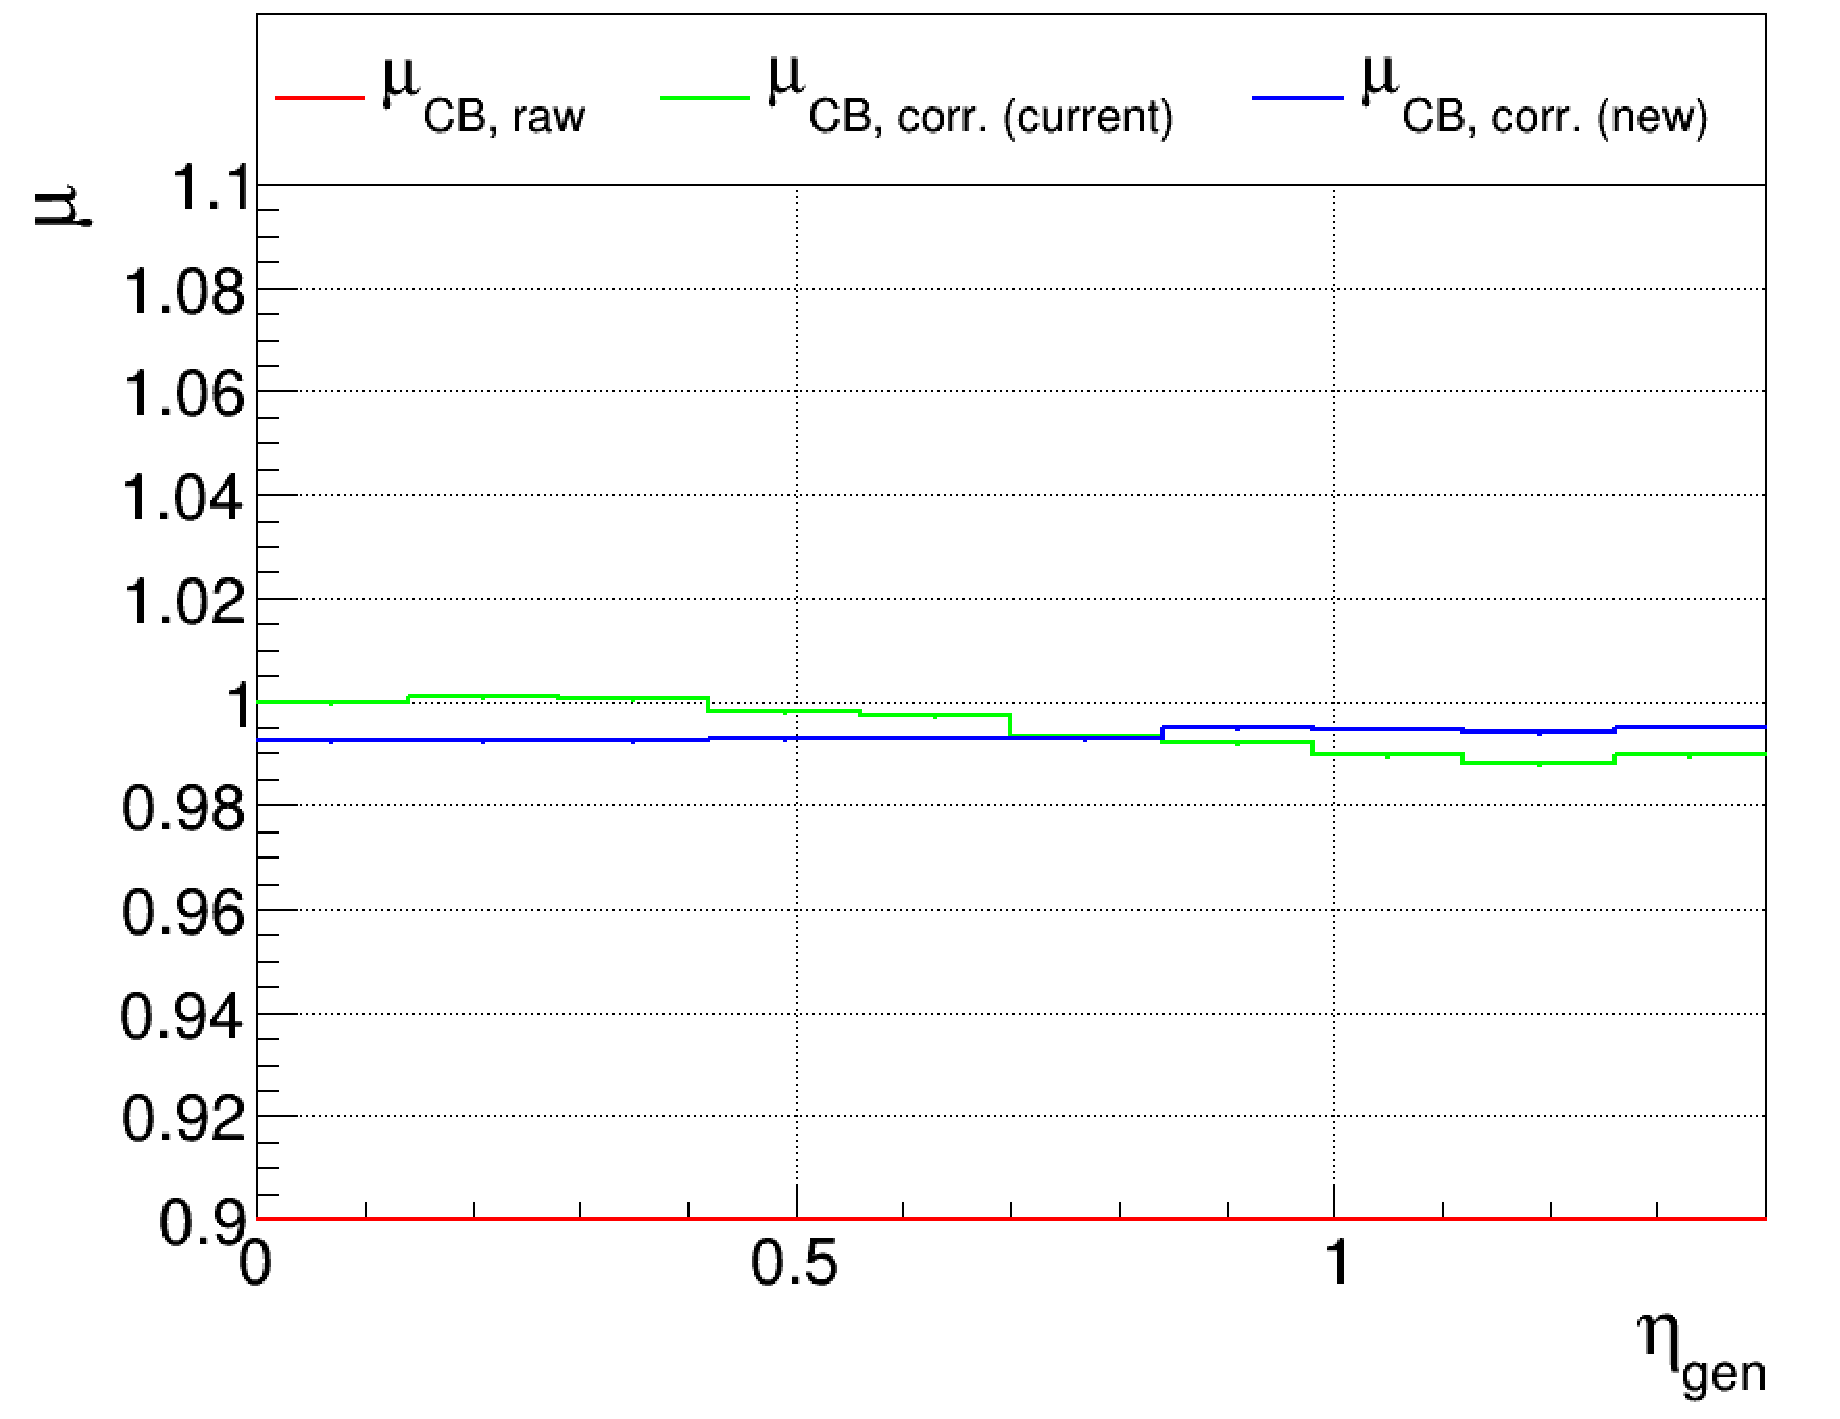
\includegraphics[width=0.495\textwidth]{./plots_pdf/ECAL_plots/plotsNOPU/EB/FULL/pdf/GENETA/EBFULL_GENETA_0005_0020_MuOverBins.pdf}
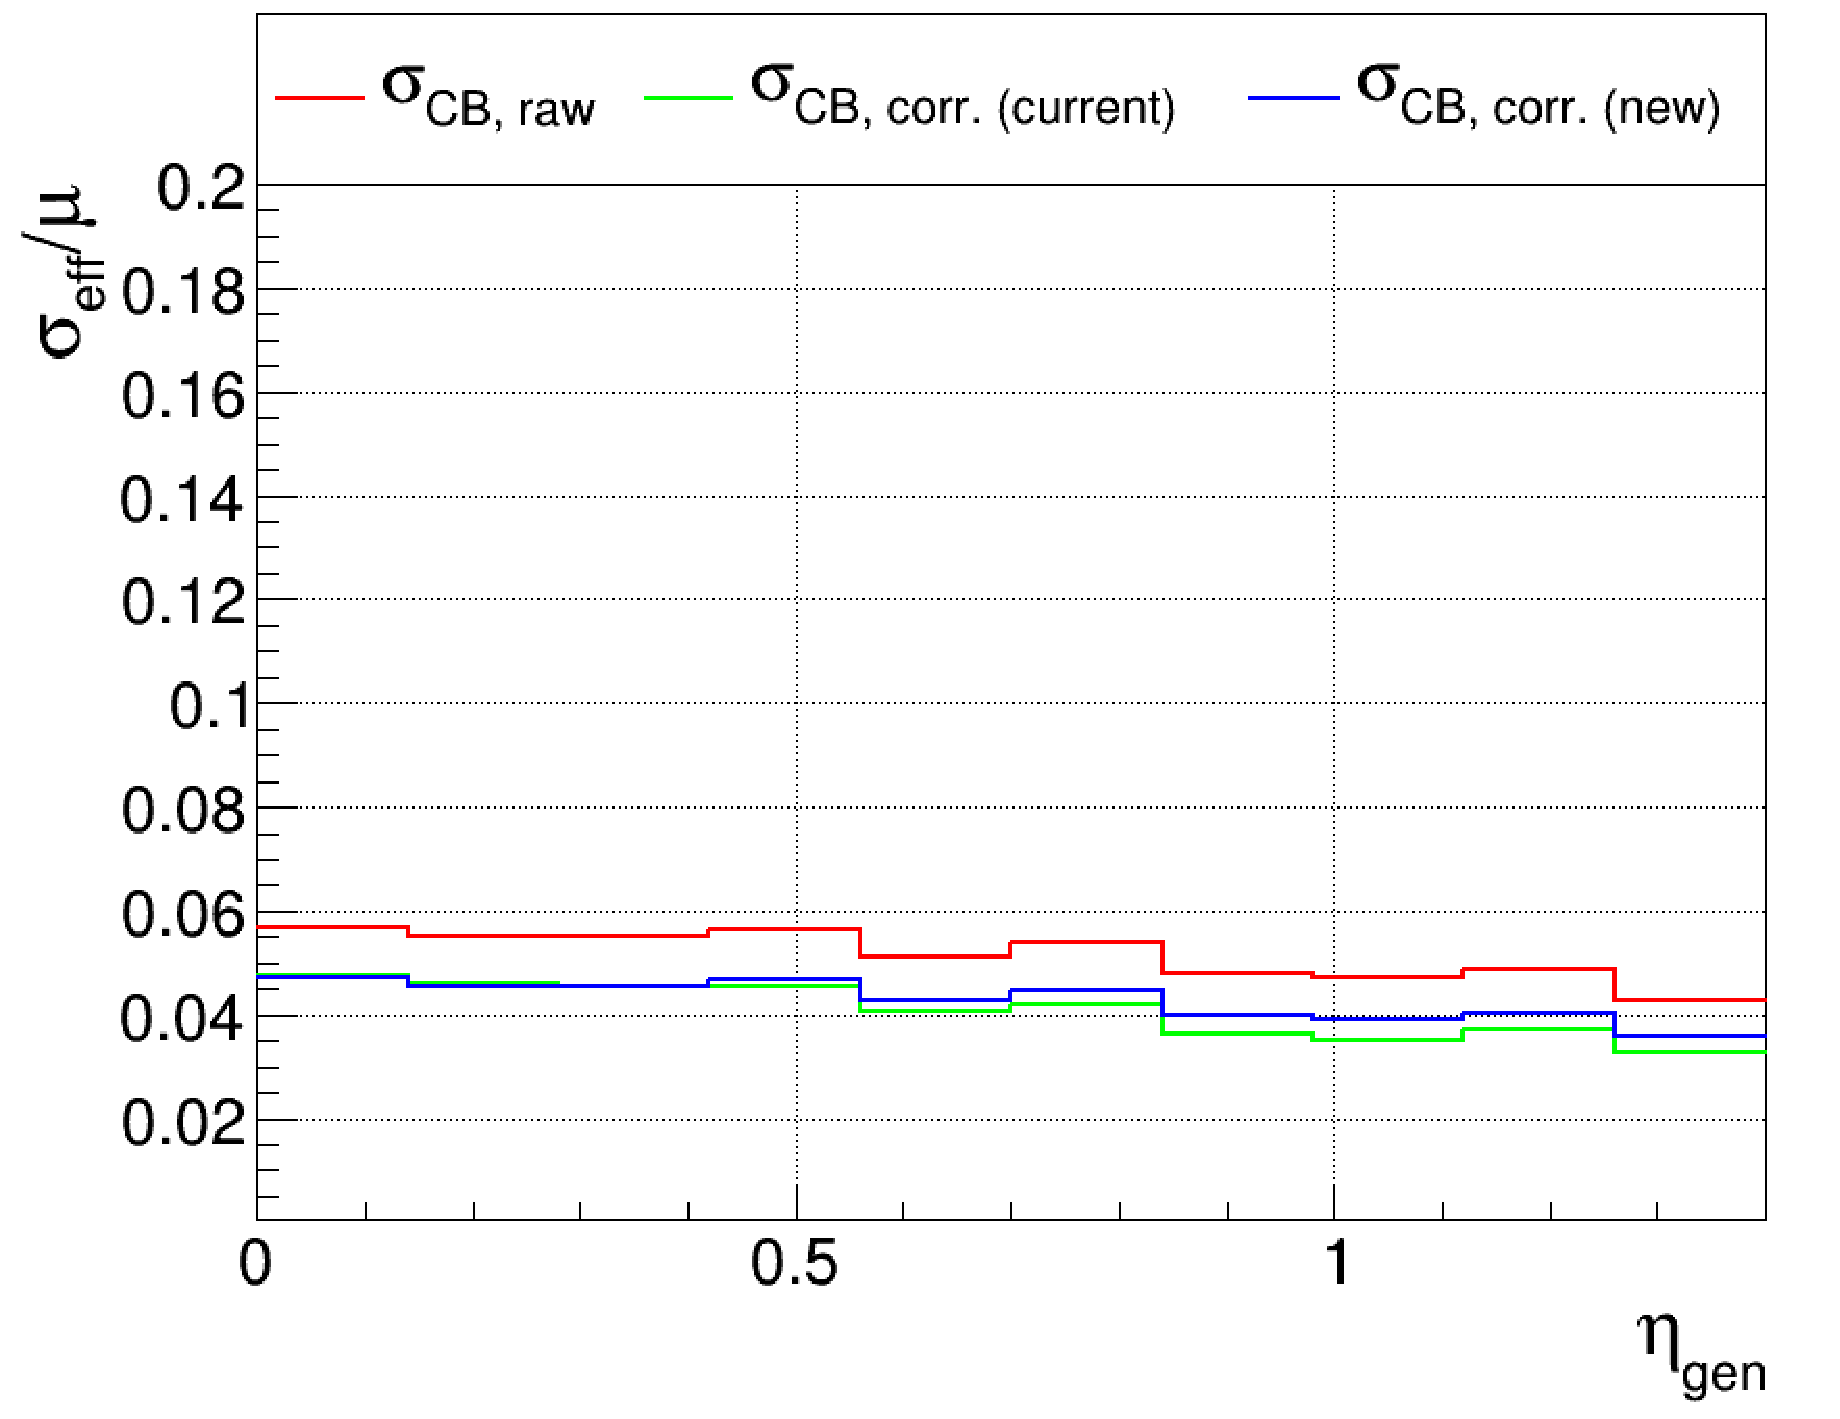
\includegraphics[width=0.495\textwidth]{./plots_pdf/ECAL_plots/plotsPU/EB/FULL/pdf/GENETA/EBFULL_GENETA_0005_0020_EffSigmaOverBins.pdf}
\caption{EB - Full Readout \pt 5-20}

%\begin{figure}
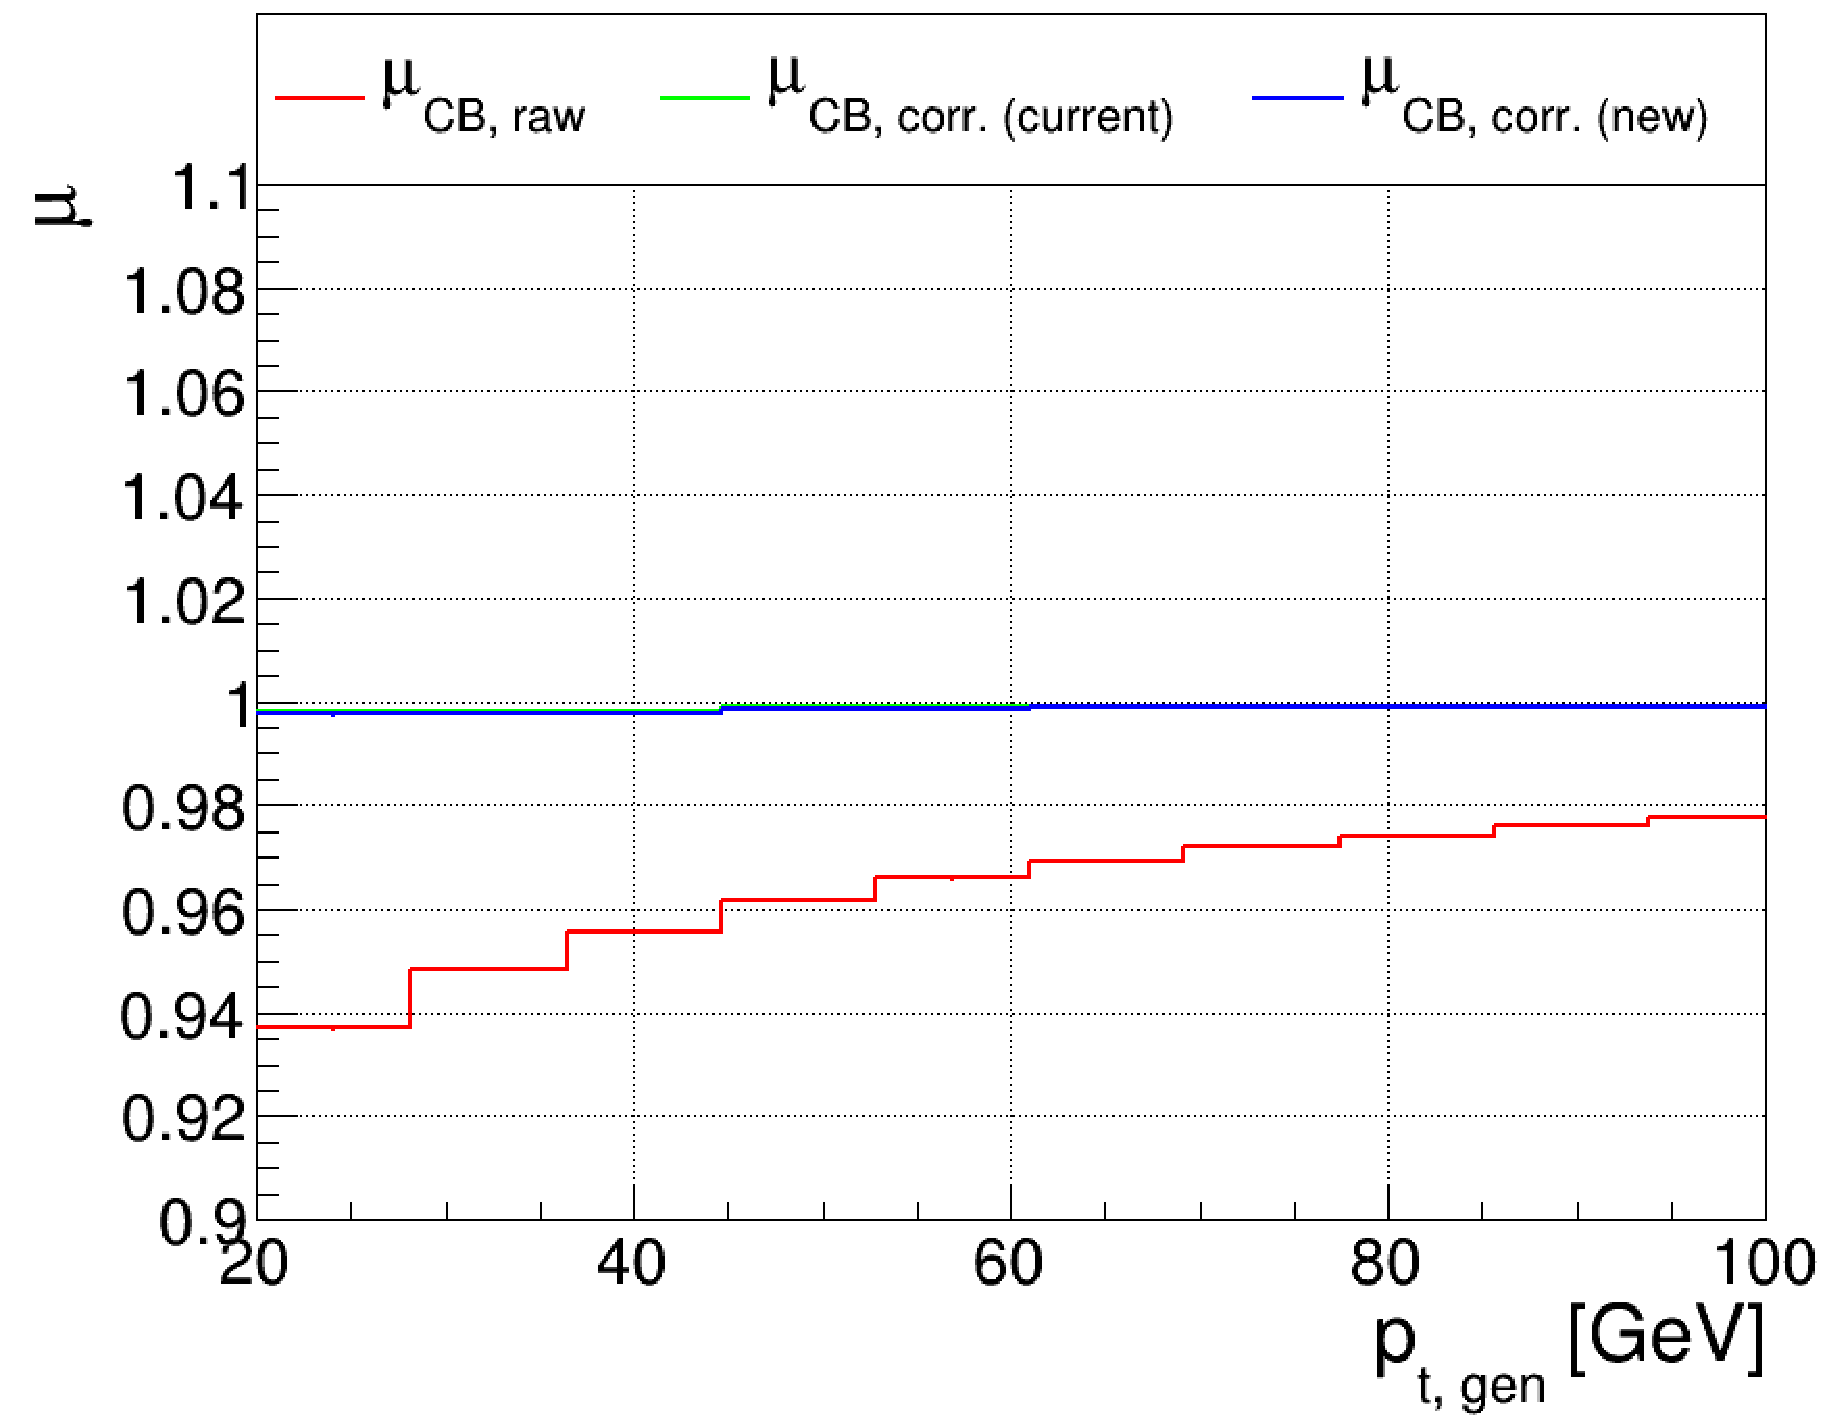
\includegraphics[width=0.495\textwidth]{./plots_pdf/ECAL_plots/plotsNOPU/EB/FULL/pdf/GENPT/EBFULL_GENPT_0020_0100_MuOverBins.pdf}
\includegraphics[width=0.495\textwidth]{./plots_pdf/ECAL_plots/plotsNOPU/EB/FULL/pdf/GENPT/EBFULL_GENPT_0020_0100_EffSigmaOverBins.pdf}

\includegraphics[width=0.495\textwidth]{./plots_pdf/ECAL_plots/plotsNOPU/EB/FULL/pdf/GENETA/EBFULL_GENETA_0020_0100_MuOverBins.pdf}
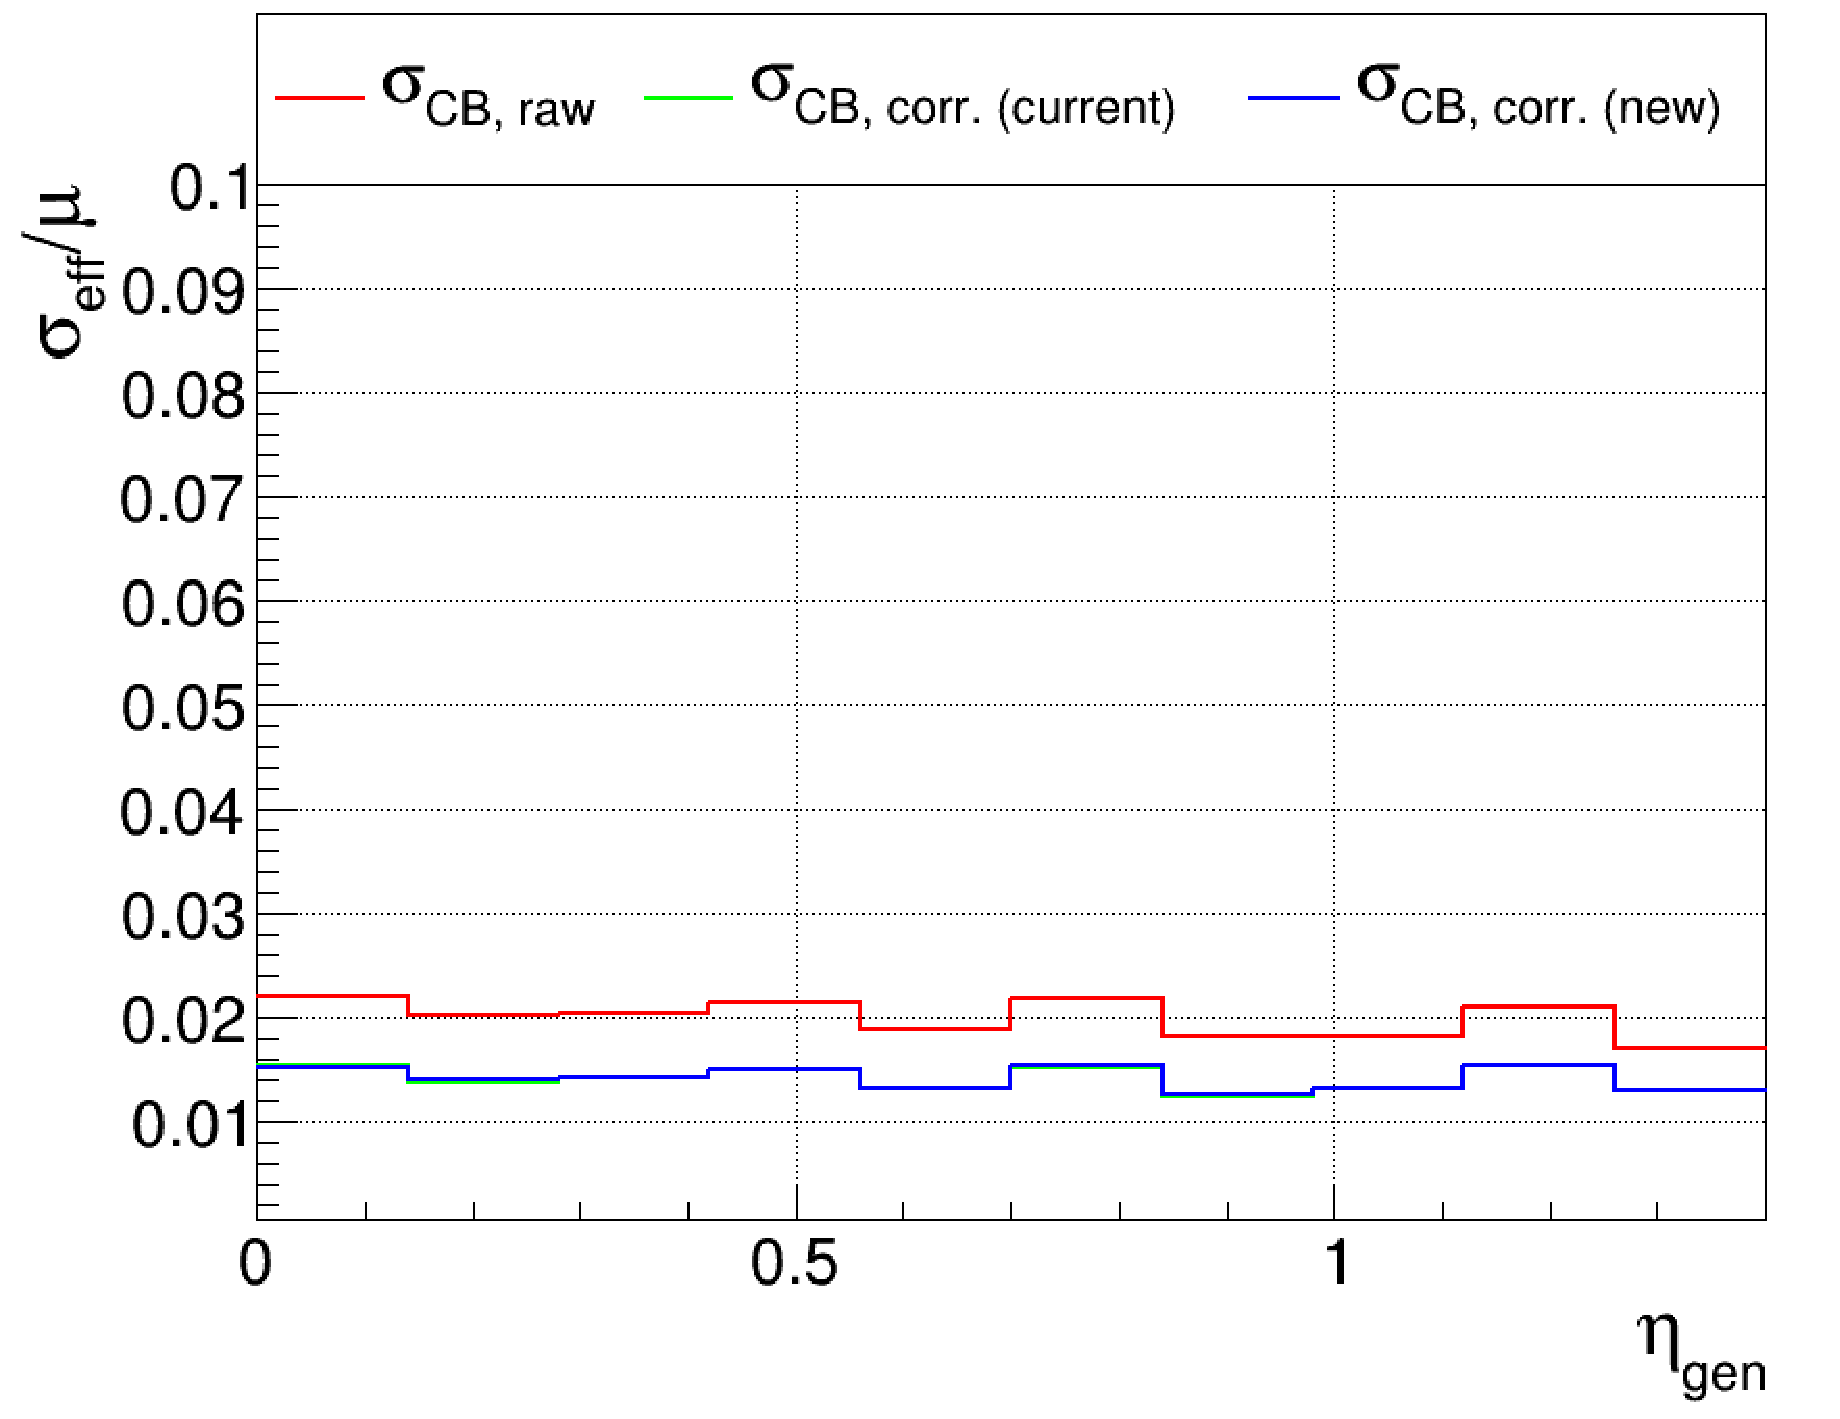
\includegraphics[width=0.495\textwidth]{./plots_pdf/ECAL_plots/plotsPU/EB/FULL/pdf/GENETA/EBFULL_GENETA_0020_0100_EffSigmaOverBins.pdf}
\caption{EB - Full Readout \pt 20-100}
\end{figure}


\begin{figure}
\includegraphics[width=0.495\textwidth]{./plots_pdf/ECAL_plots/plotsNOPU/EB/FULL/pdf/GENPT/EBFULL_GENPT_0100_0300_MuOverBins.pdf}
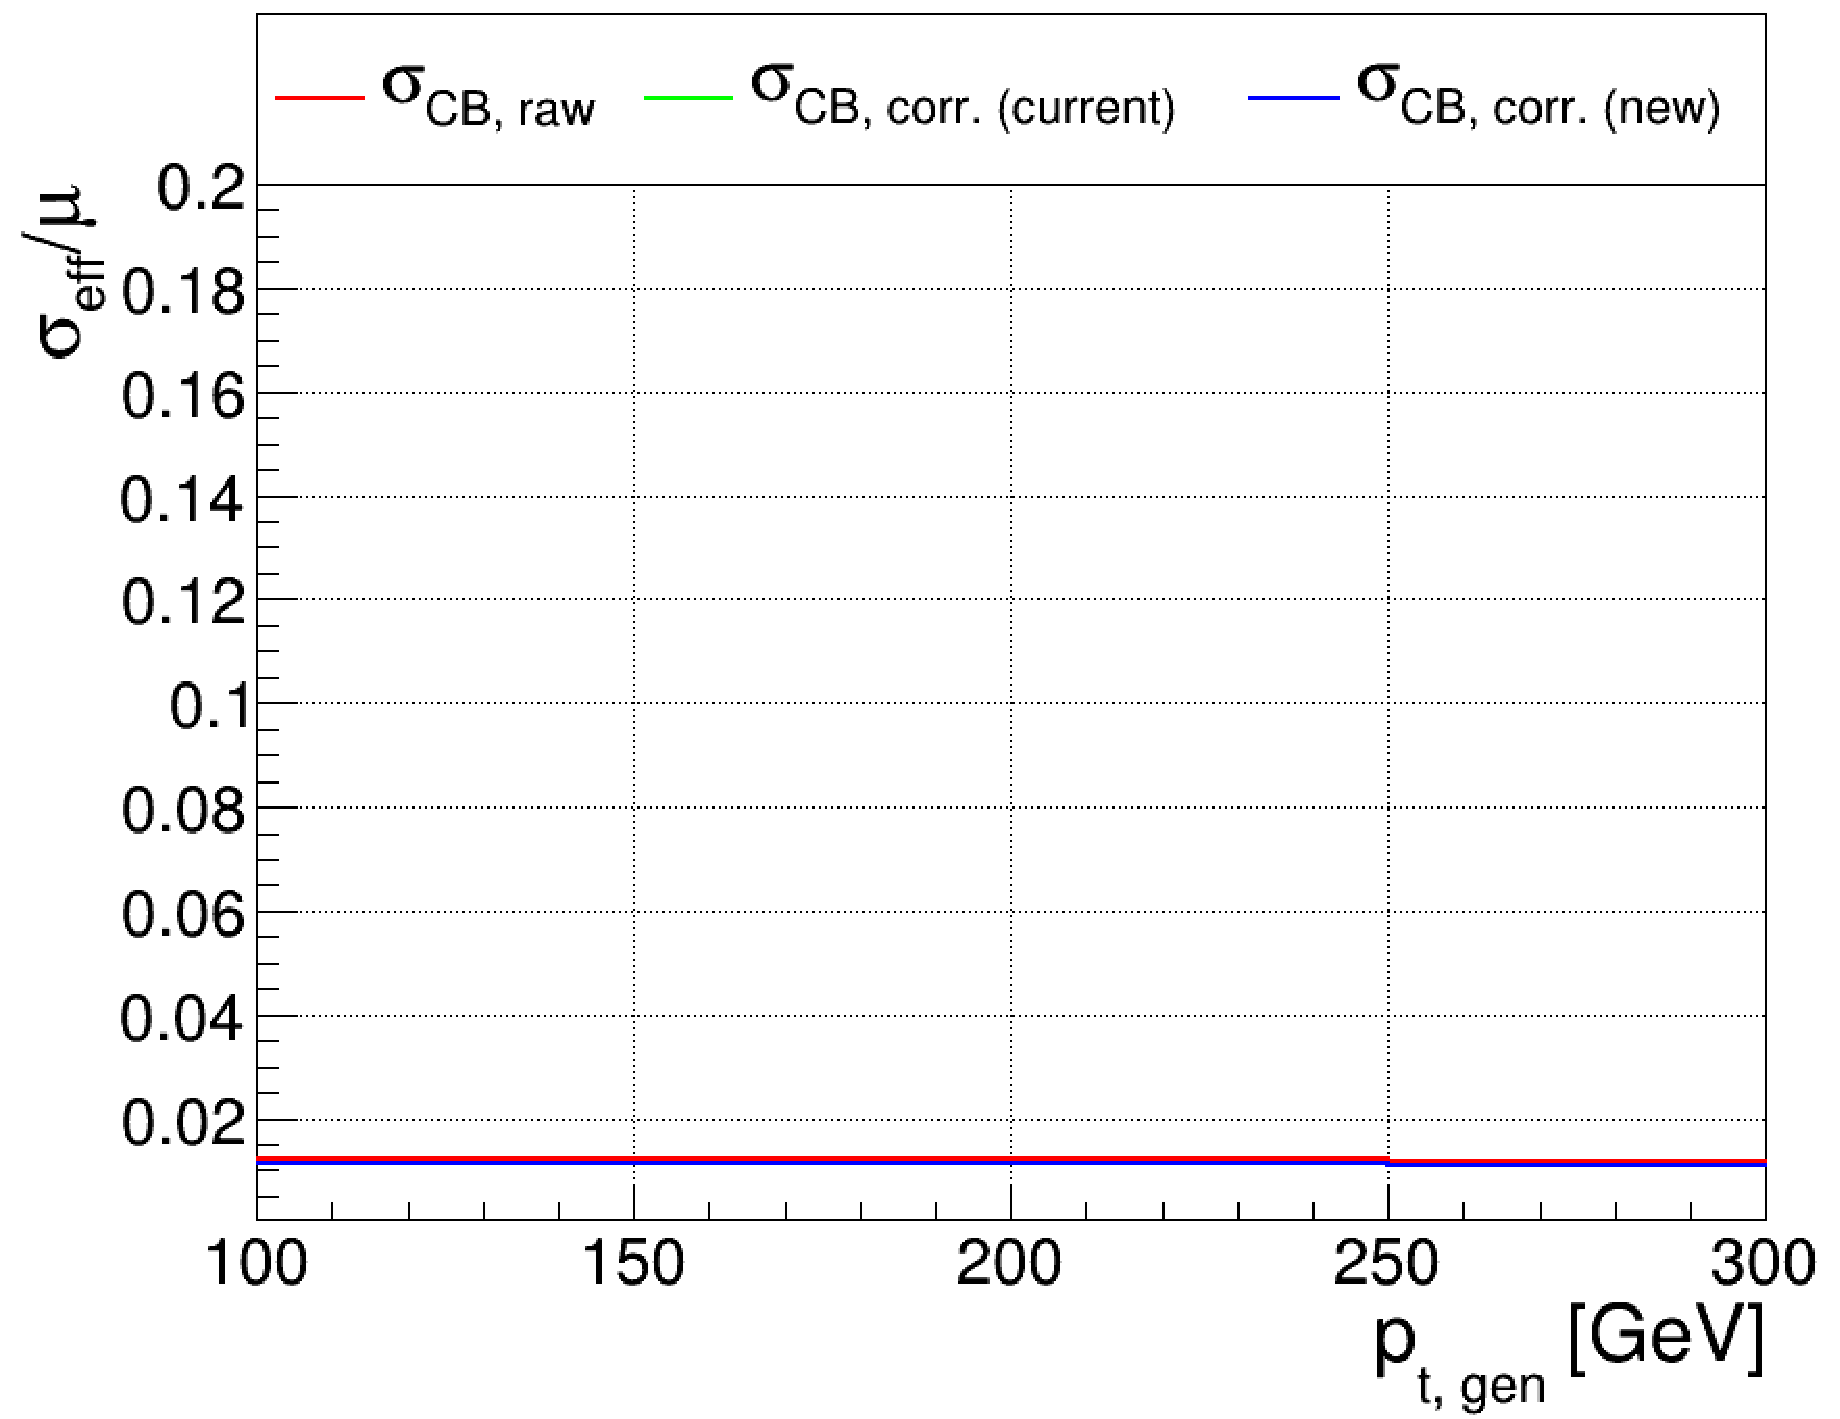
\includegraphics[width=0.495\textwidth]{./plots_pdf/ECAL_plots/plotsPU/EB/FULL/pdf/GENPT/EBFULL_GENPT_0100_0300_EffSigmaOverBins.pdf}


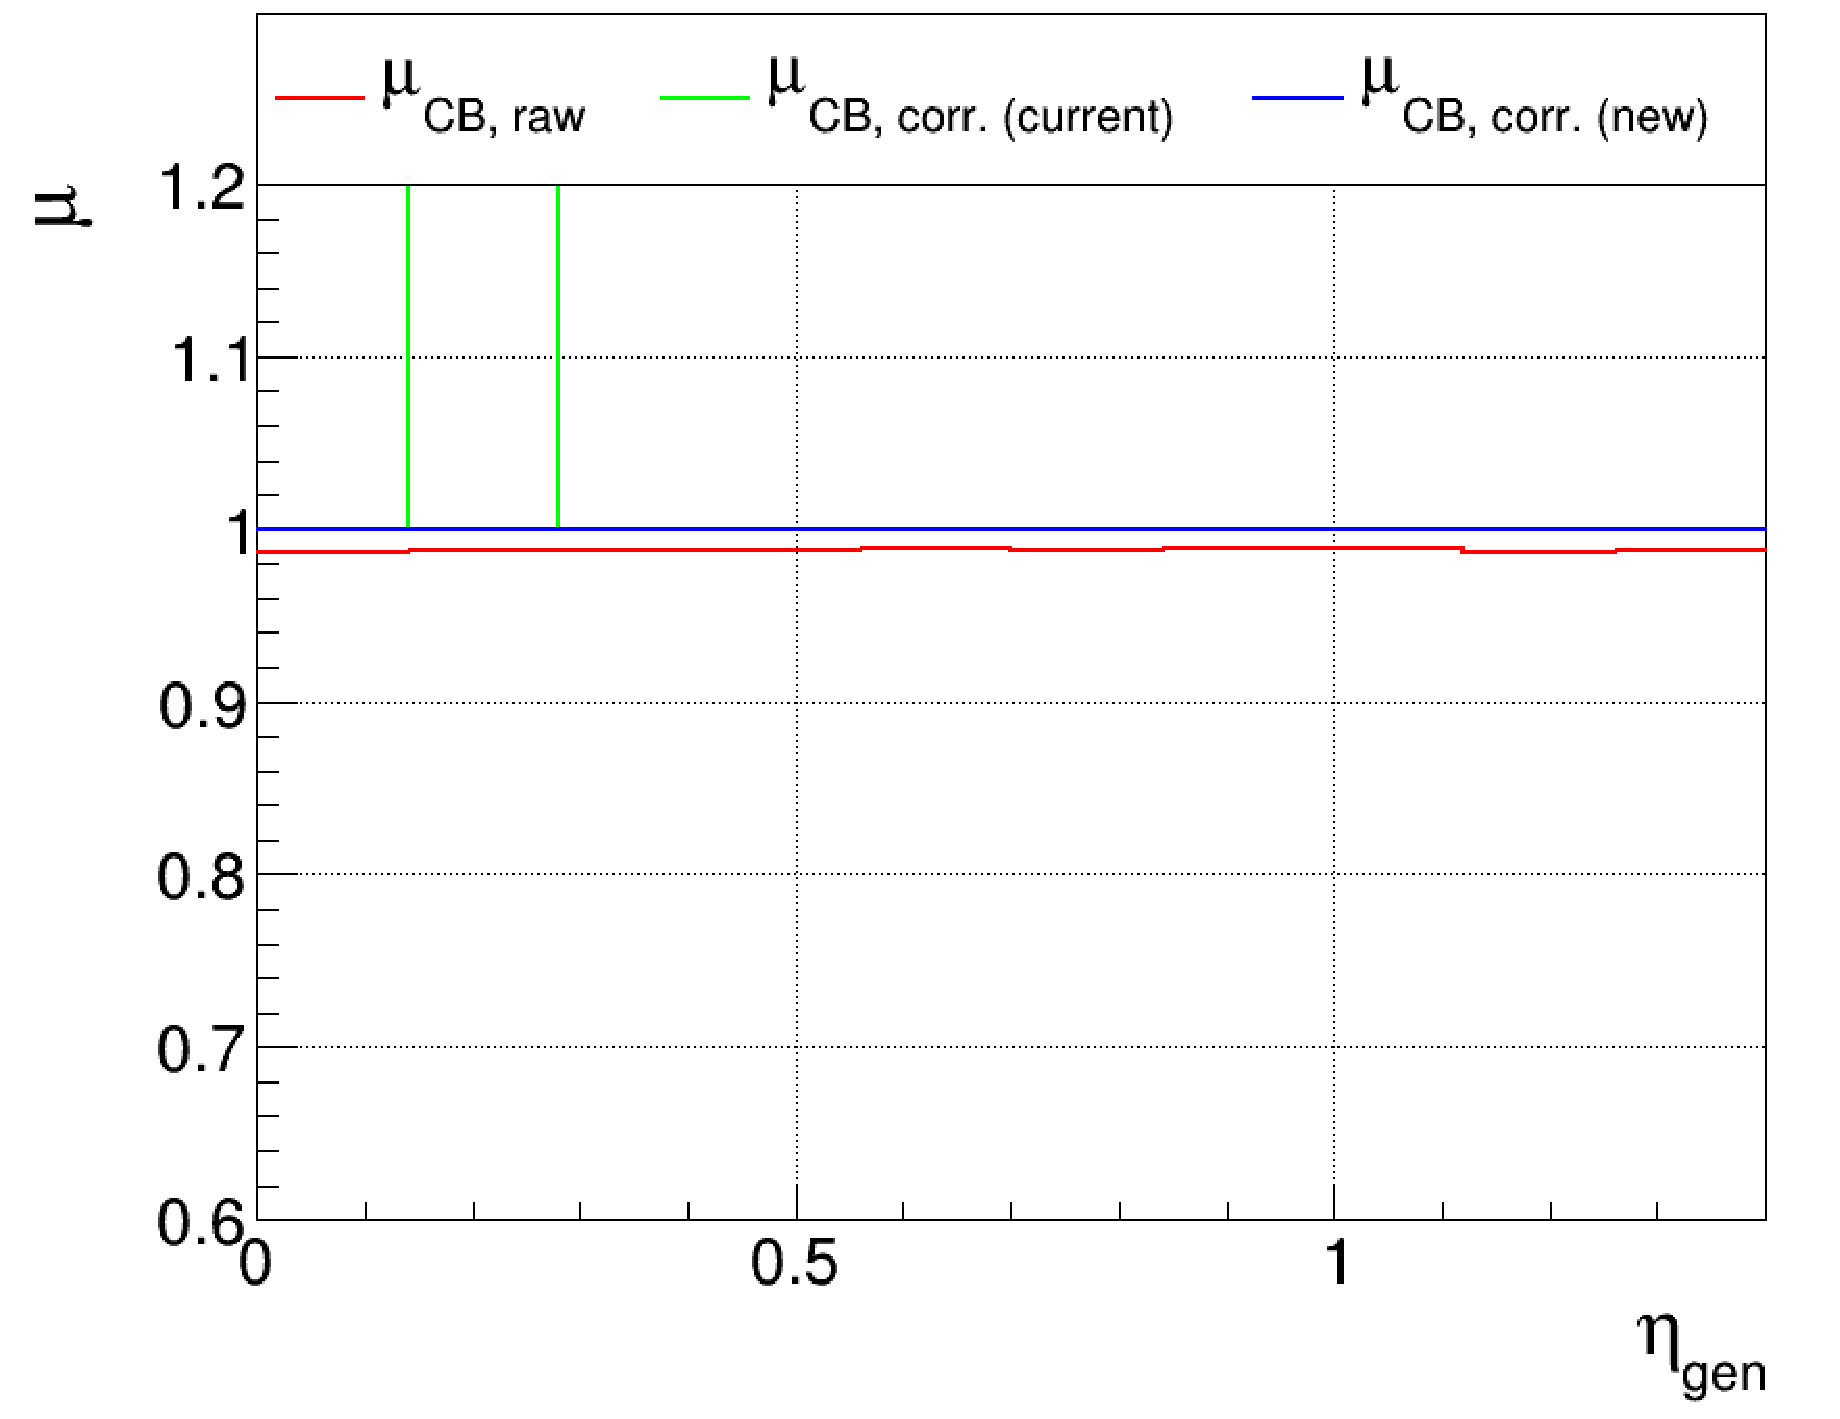
\includegraphics[width=0.495\textwidth]{./plots_pdf/ECAL_plots/plotsNOPU/EB/FULL/pdf/GENETA/EBFULL_GENETA_0100_0300_MuOverBins.pdf}
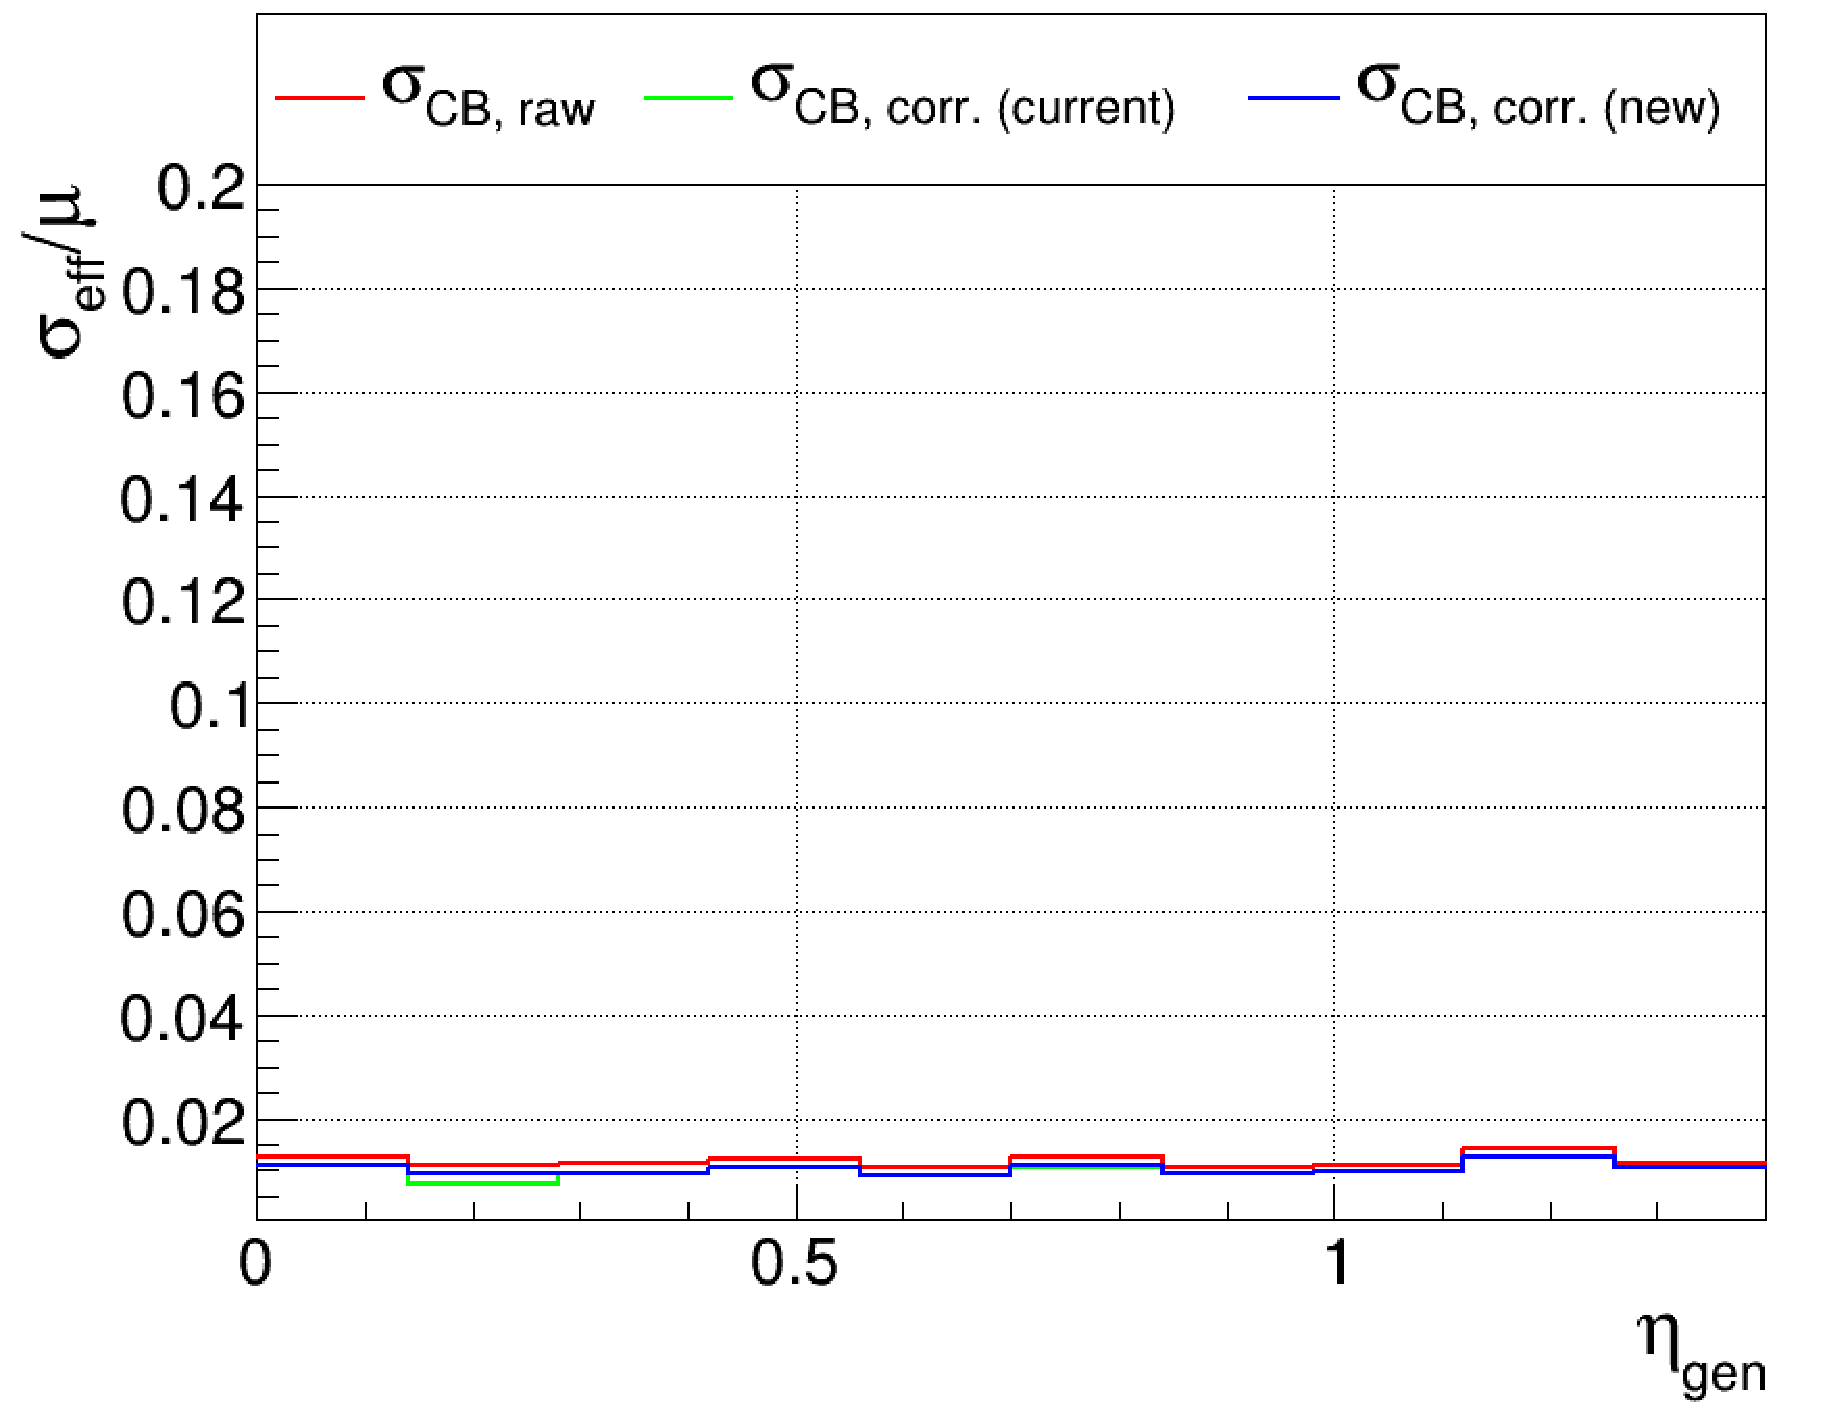
\includegraphics[width=0.495\textwidth]{./plots_pdf/ECAL_plots/plotsNOPU/EB/FULL/pdf/GENETA/EBFULL_GENETA_0100_0300_EffSigmaOverBins.pdf}
\caption{EB - Full Readout \pt 100-300}
\end{figure}




\begin{figure}
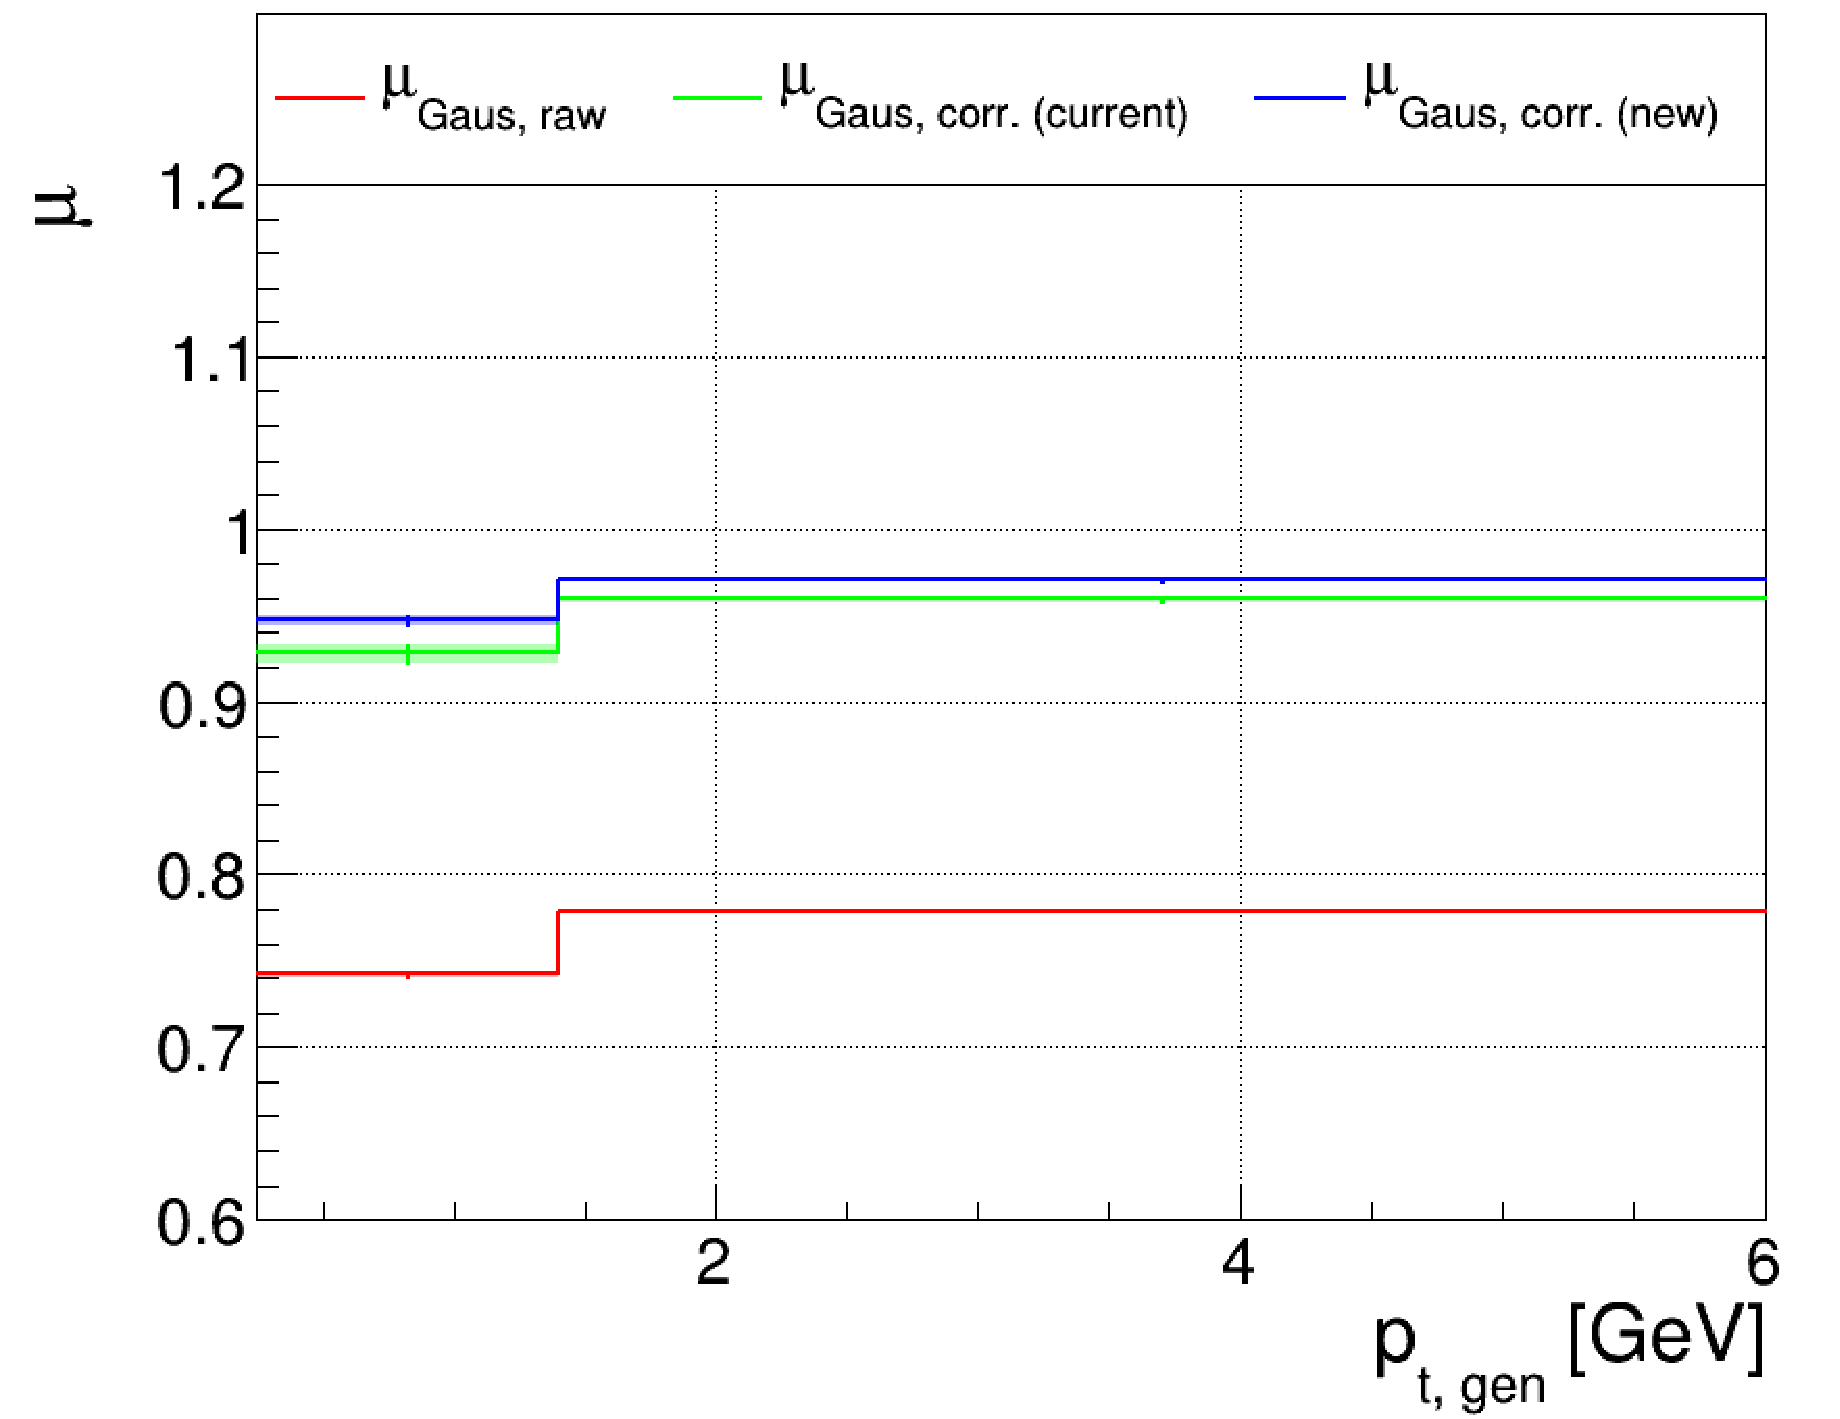
\includegraphics[width=0.495\textwidth]{./ECAL_plots/plotsNOPU/EB/ZS/pdf/GENPT/EBZS_GENPT_0000_0006_MuOverBins.pdf}
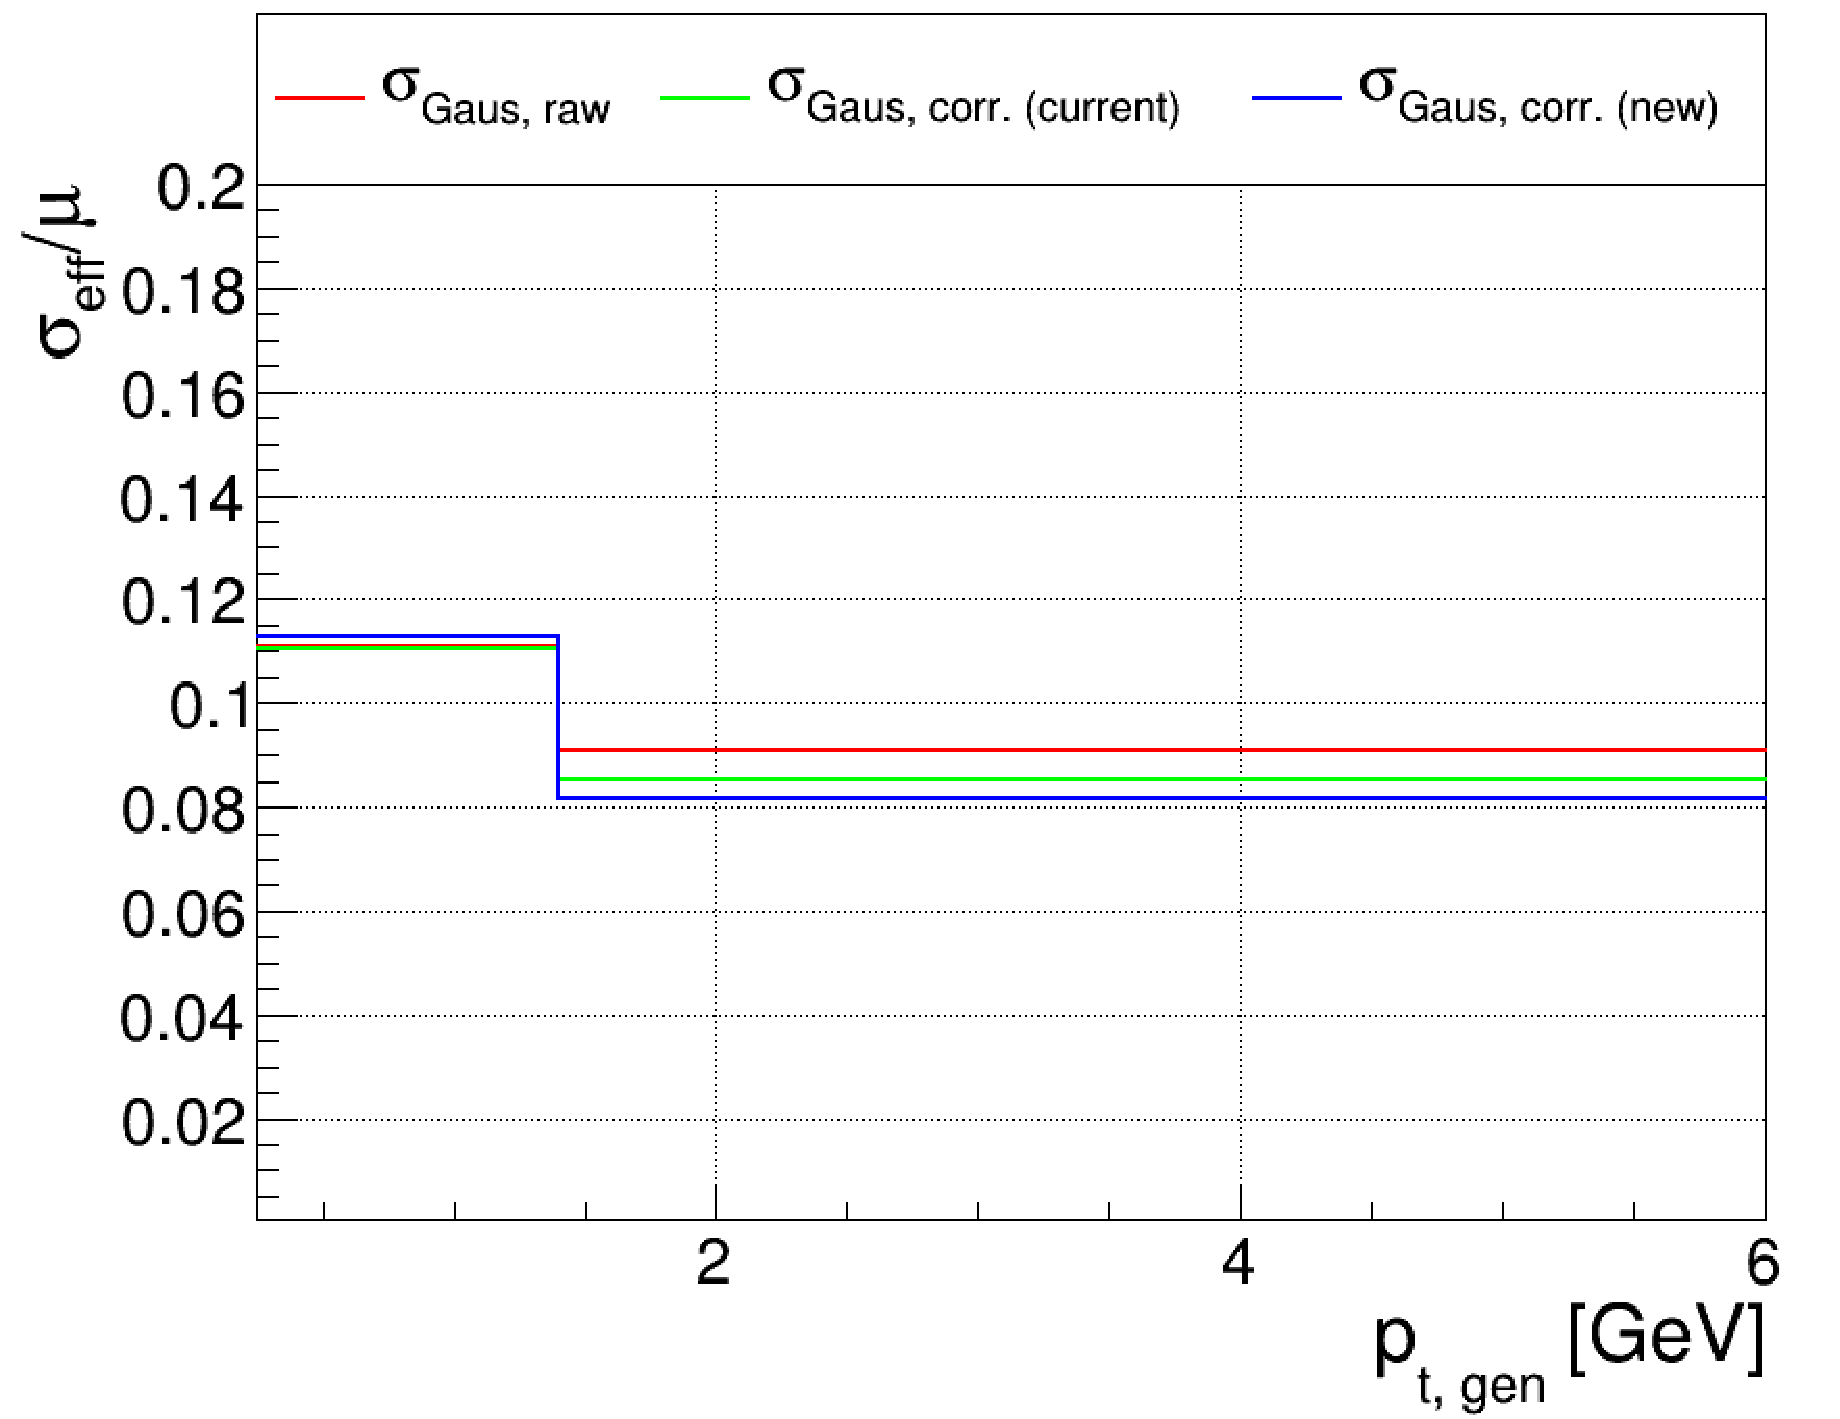
\includegraphics[width=0.495\textwidth]{./ECAL_plots/plotsNOPU/EB/ZS/pdf/GENPT/EBZS_GENPT_0000_0006_EffSigmaOverBins.pdf}
%\caption{EB - ZSl Readout pt 0-6}
%\end{figure}
%\begin{figure}
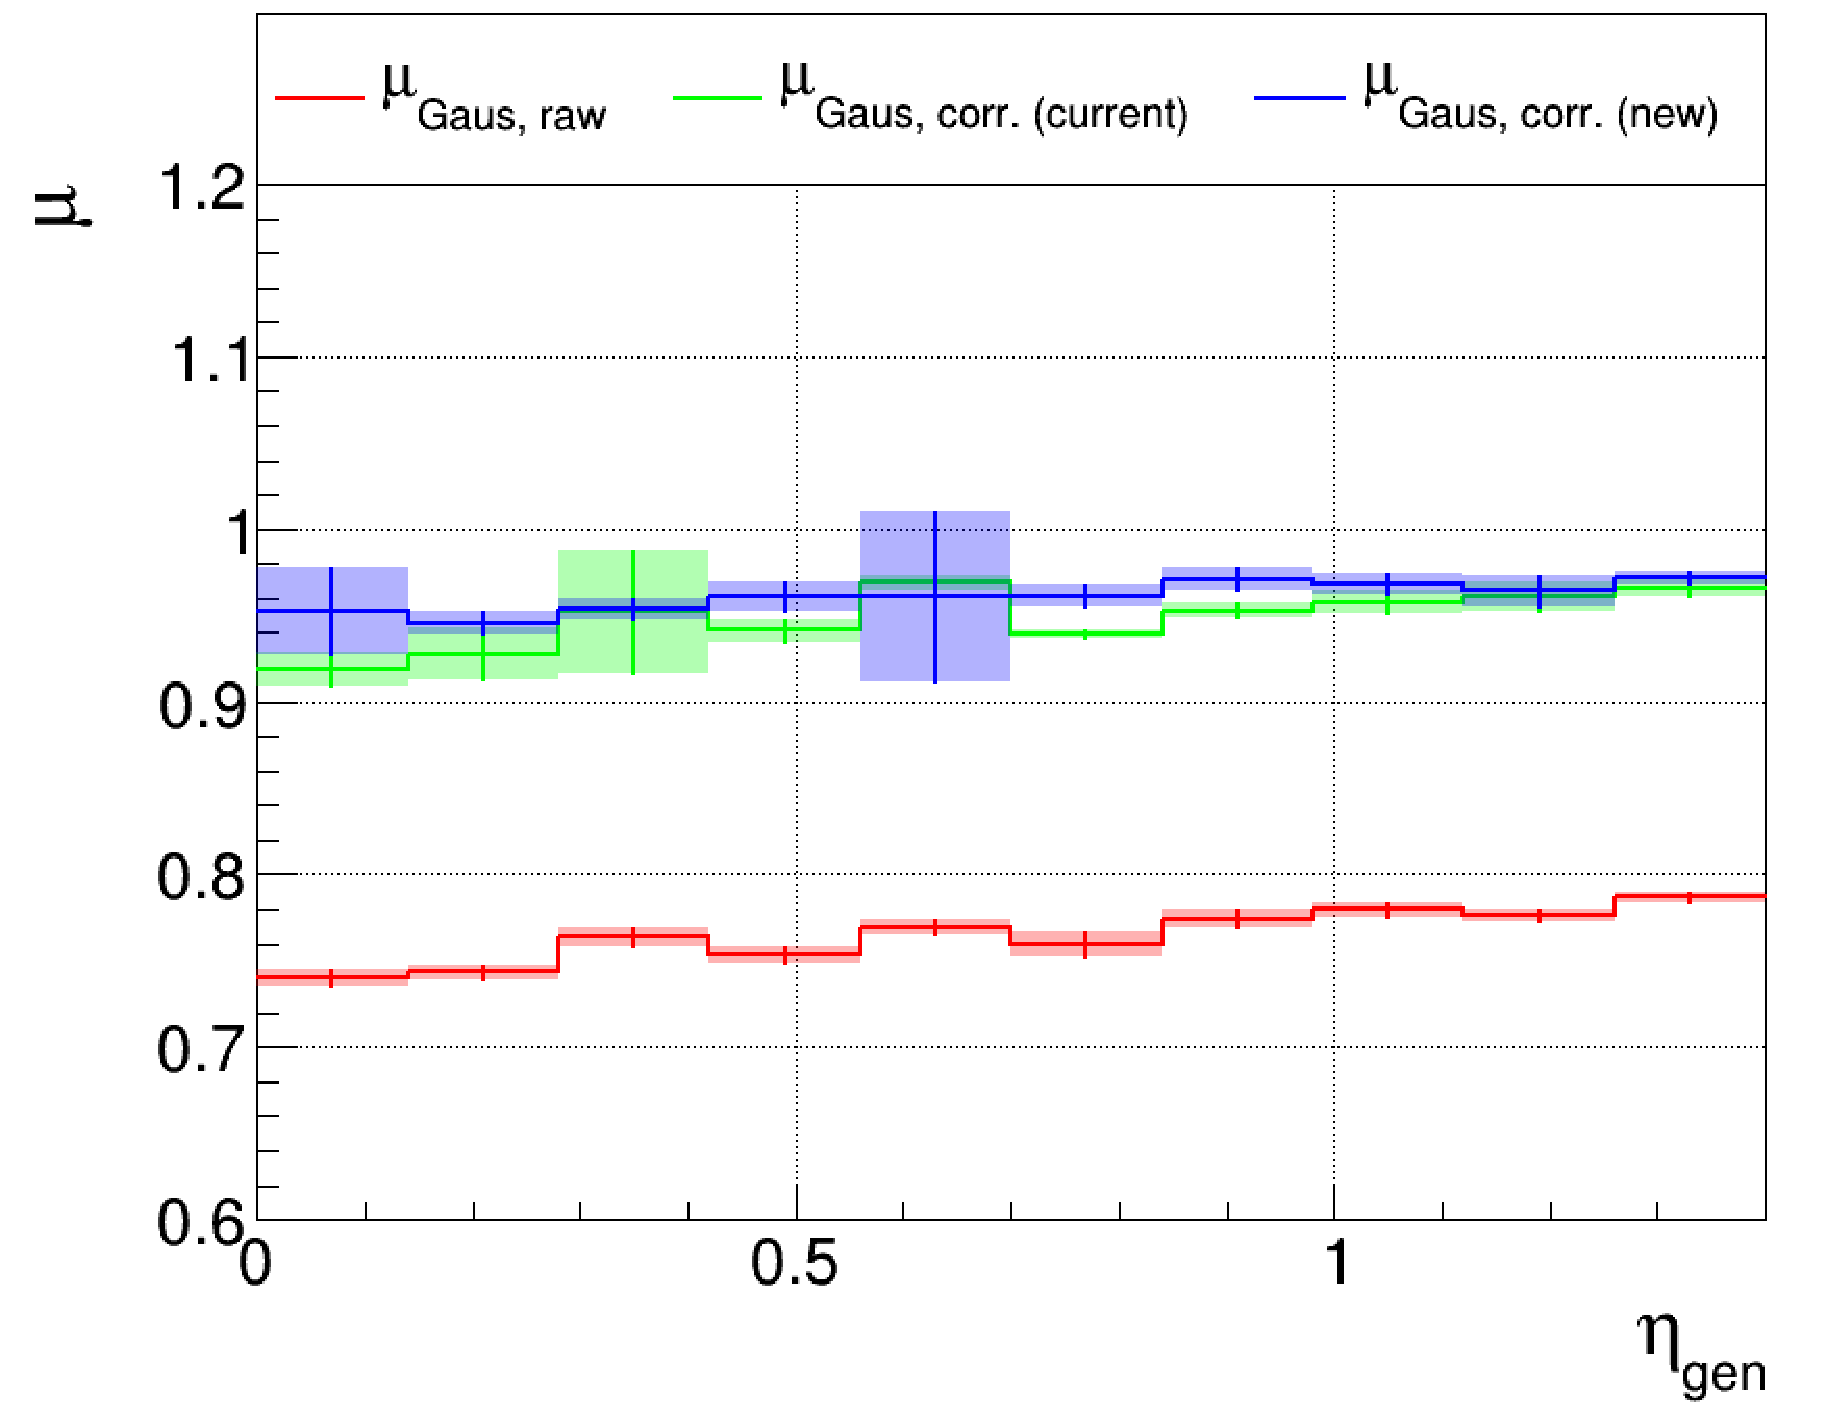
\includegraphics[width=0.495\textwidth]{./ECAL_plots/plotsNOPU/EB/ZS/pdf/GENETA/EBZS_GENETA_0000_0006_MuOverBins.pdf}
\includegraphics[width=0.495\textwidth]{./ECAL_plots/plotsNOPU/EB/ZS/pdf/GENETA/EBZS_GENETA_0000_0006_EffSigmaOverBins.pdf}
\caption{EB - ZS Readout pt 0-6}
\end{figure}


\begin{figure}
\includegraphics[width=0.495\textwidth]{./ECAL_plots/plotsNOPU/EB/ZS/pdf/GENPT/EBZS_GENPT_0006_0025_MuOverBins.pdf}
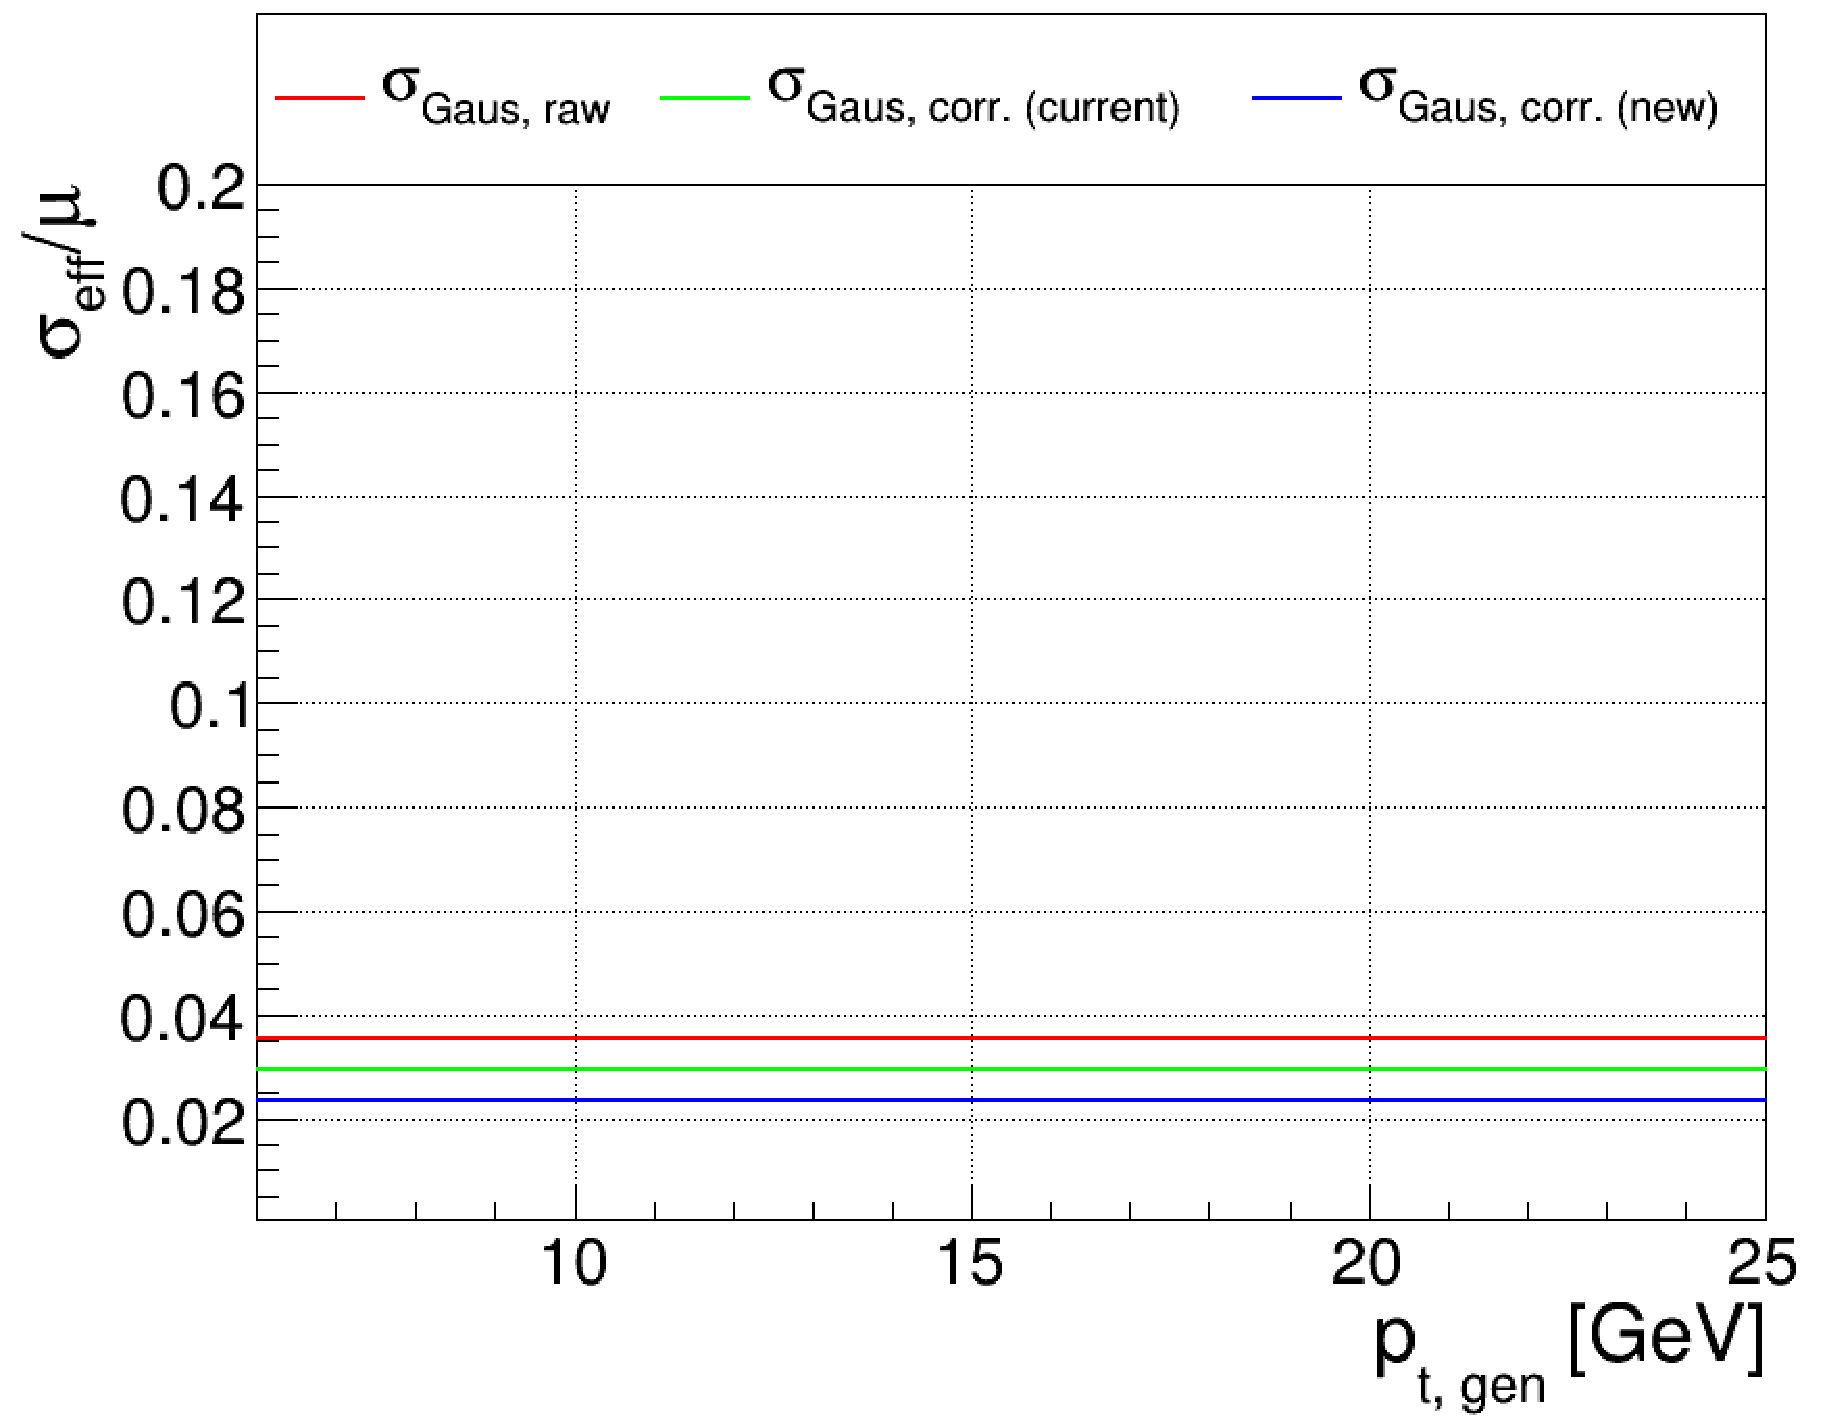
\includegraphics[width=0.495\textwidth]{./ECAL_plots/plotsNOPU/EB/ZS/pdf/GENPT/EBZS_GENPT_0006_0025_EffSigmaOverBins.pdf}
%\caption{EB - ZS Readout pt 6-25}
%\end{figure}
%\begin{figure}
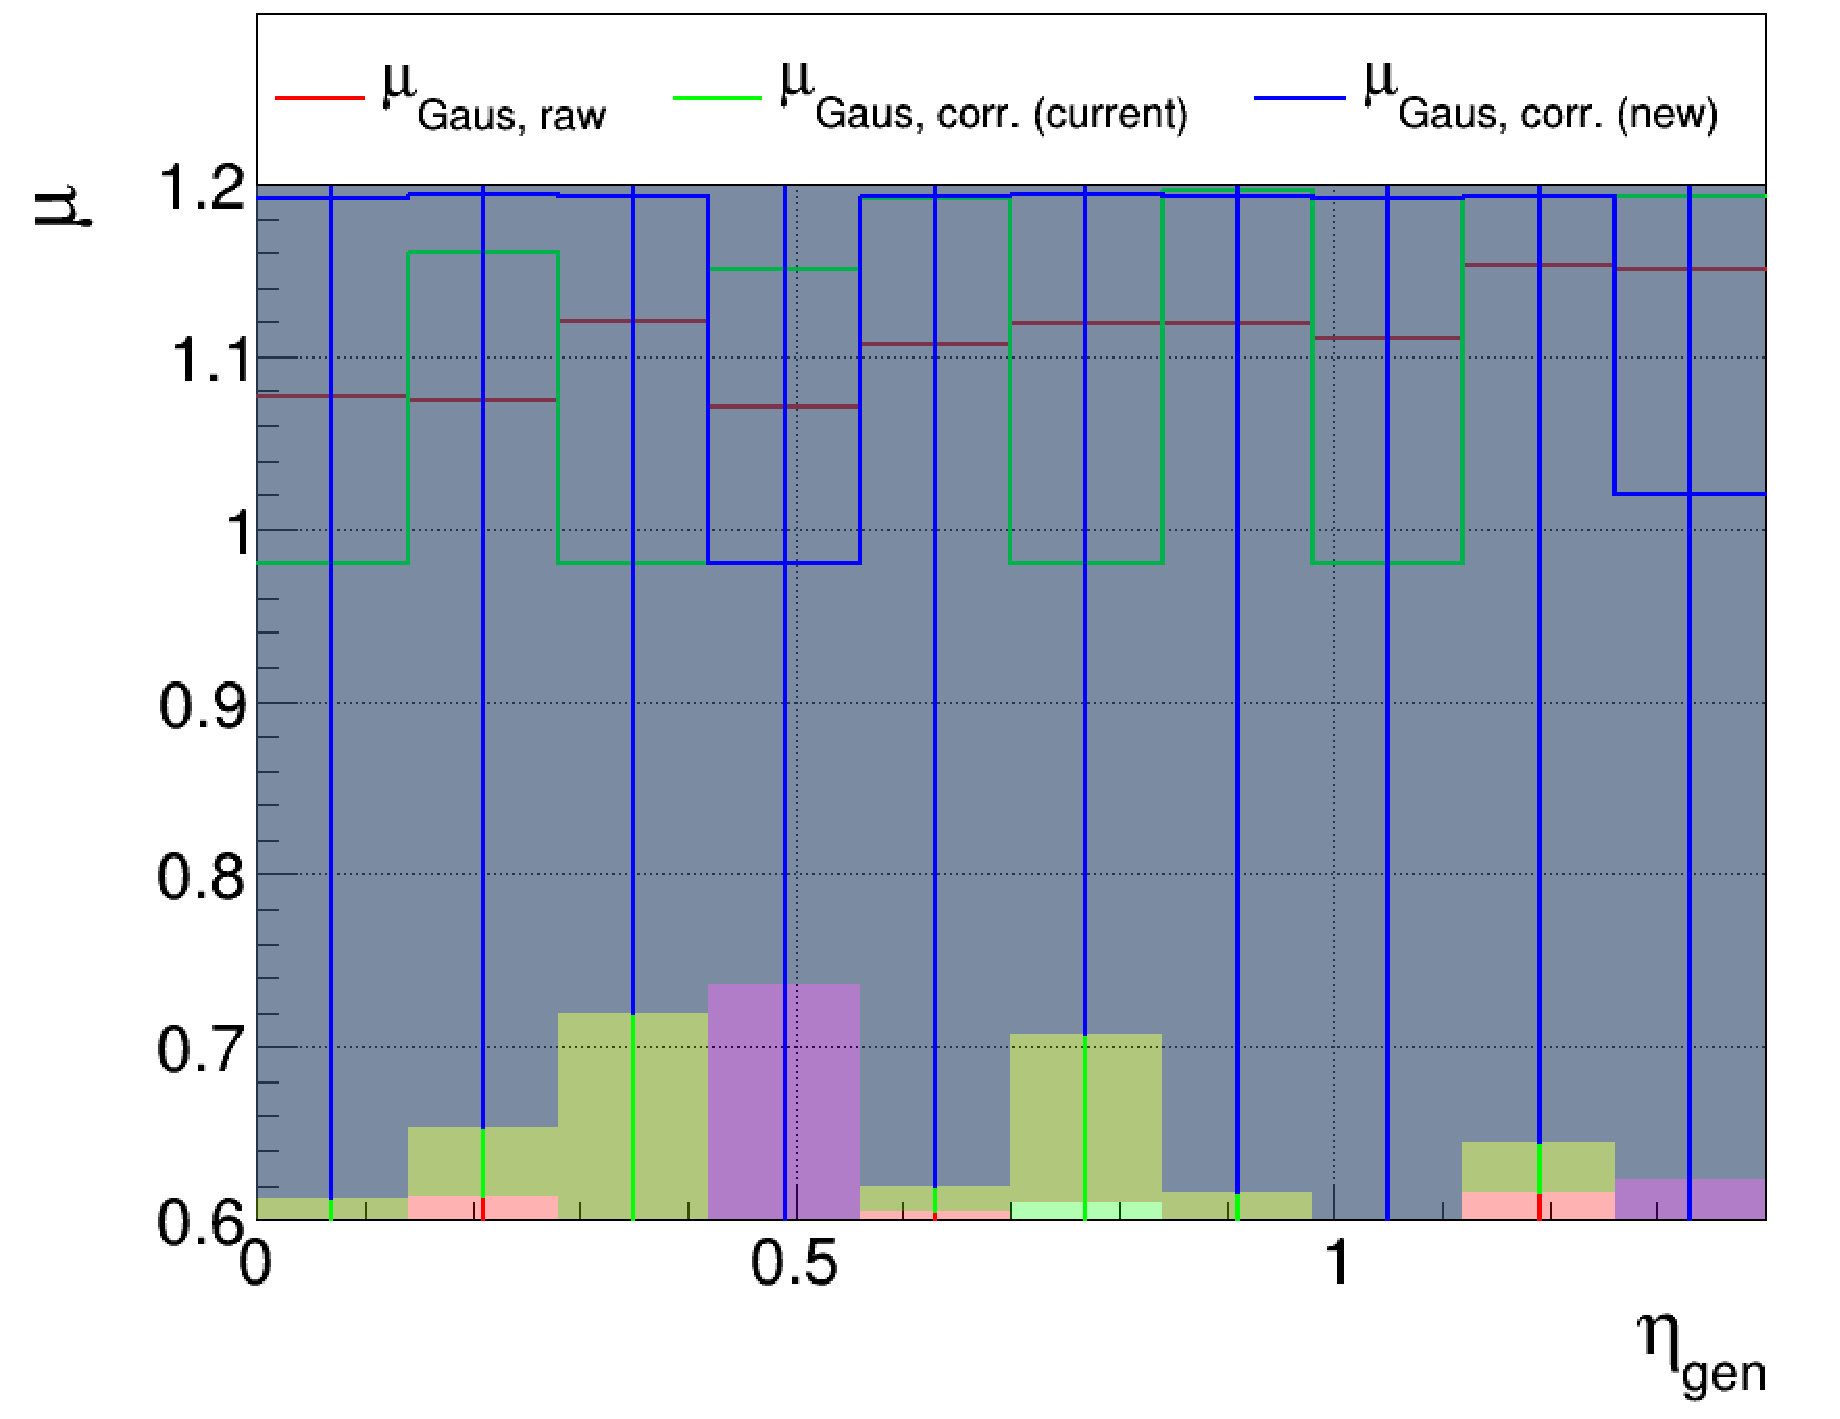
\includegraphics[width=0.495\textwidth]{./ECAL_plots/plotsNOPU/EB/ZS/pdf/GENETA/EBZS_GENETA_0006_0025_MuOverBins.pdf}
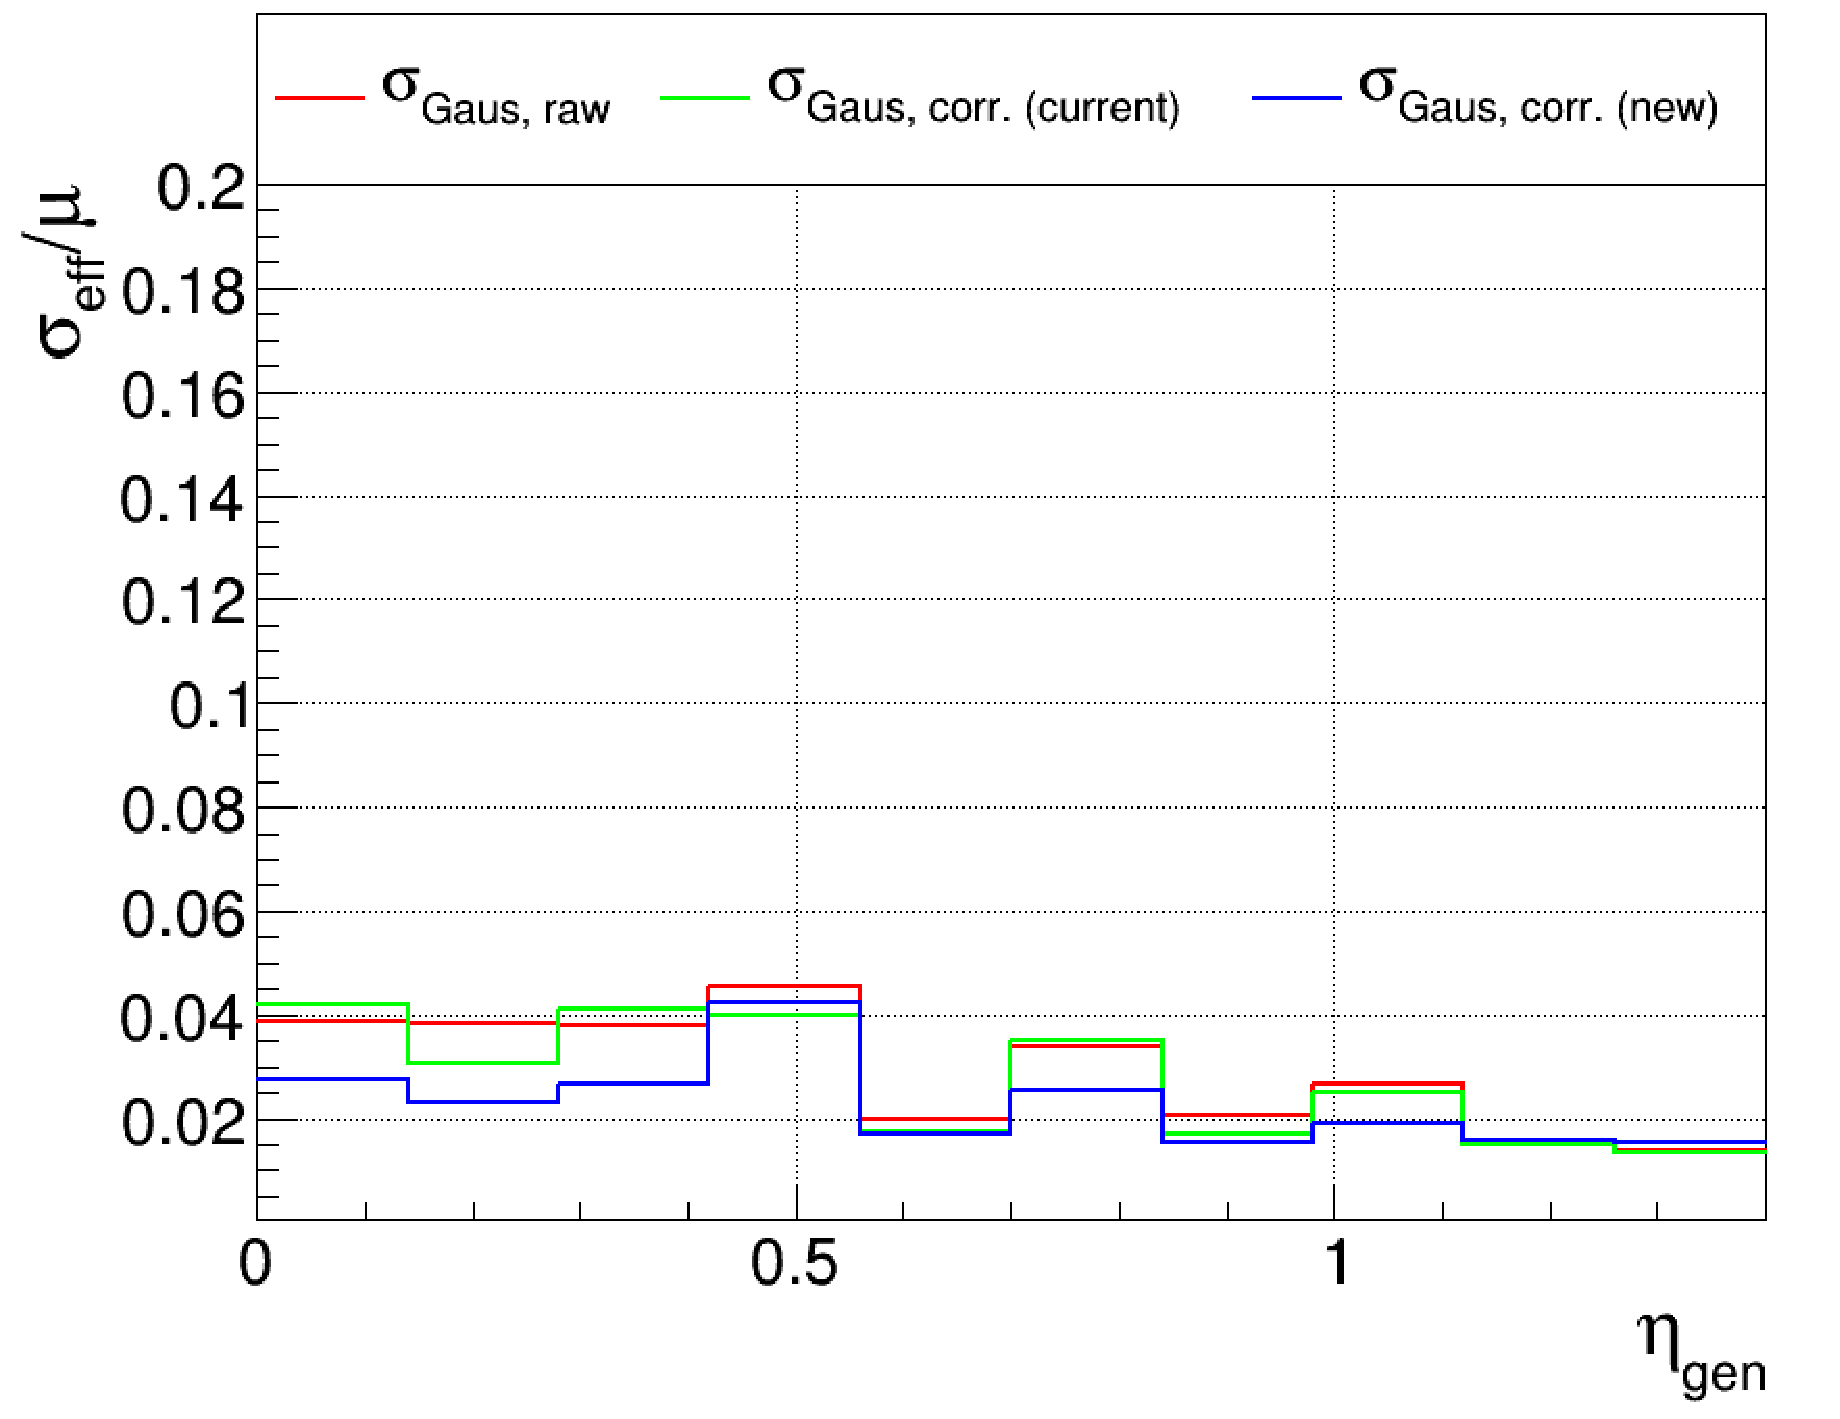
\includegraphics[width=0.495\textwidth]{./ECAL_plots/plotsNOPU/EB/ZS/pdf/GENETA/EBZS_GENETA_0006_0025_EffSigmaOverBins.pdf}
\caption{EB - ZS Readout pt 6-25}
\end{figure}






\subsection{ECAL Endcap}
in EE region:
\begin{figure}
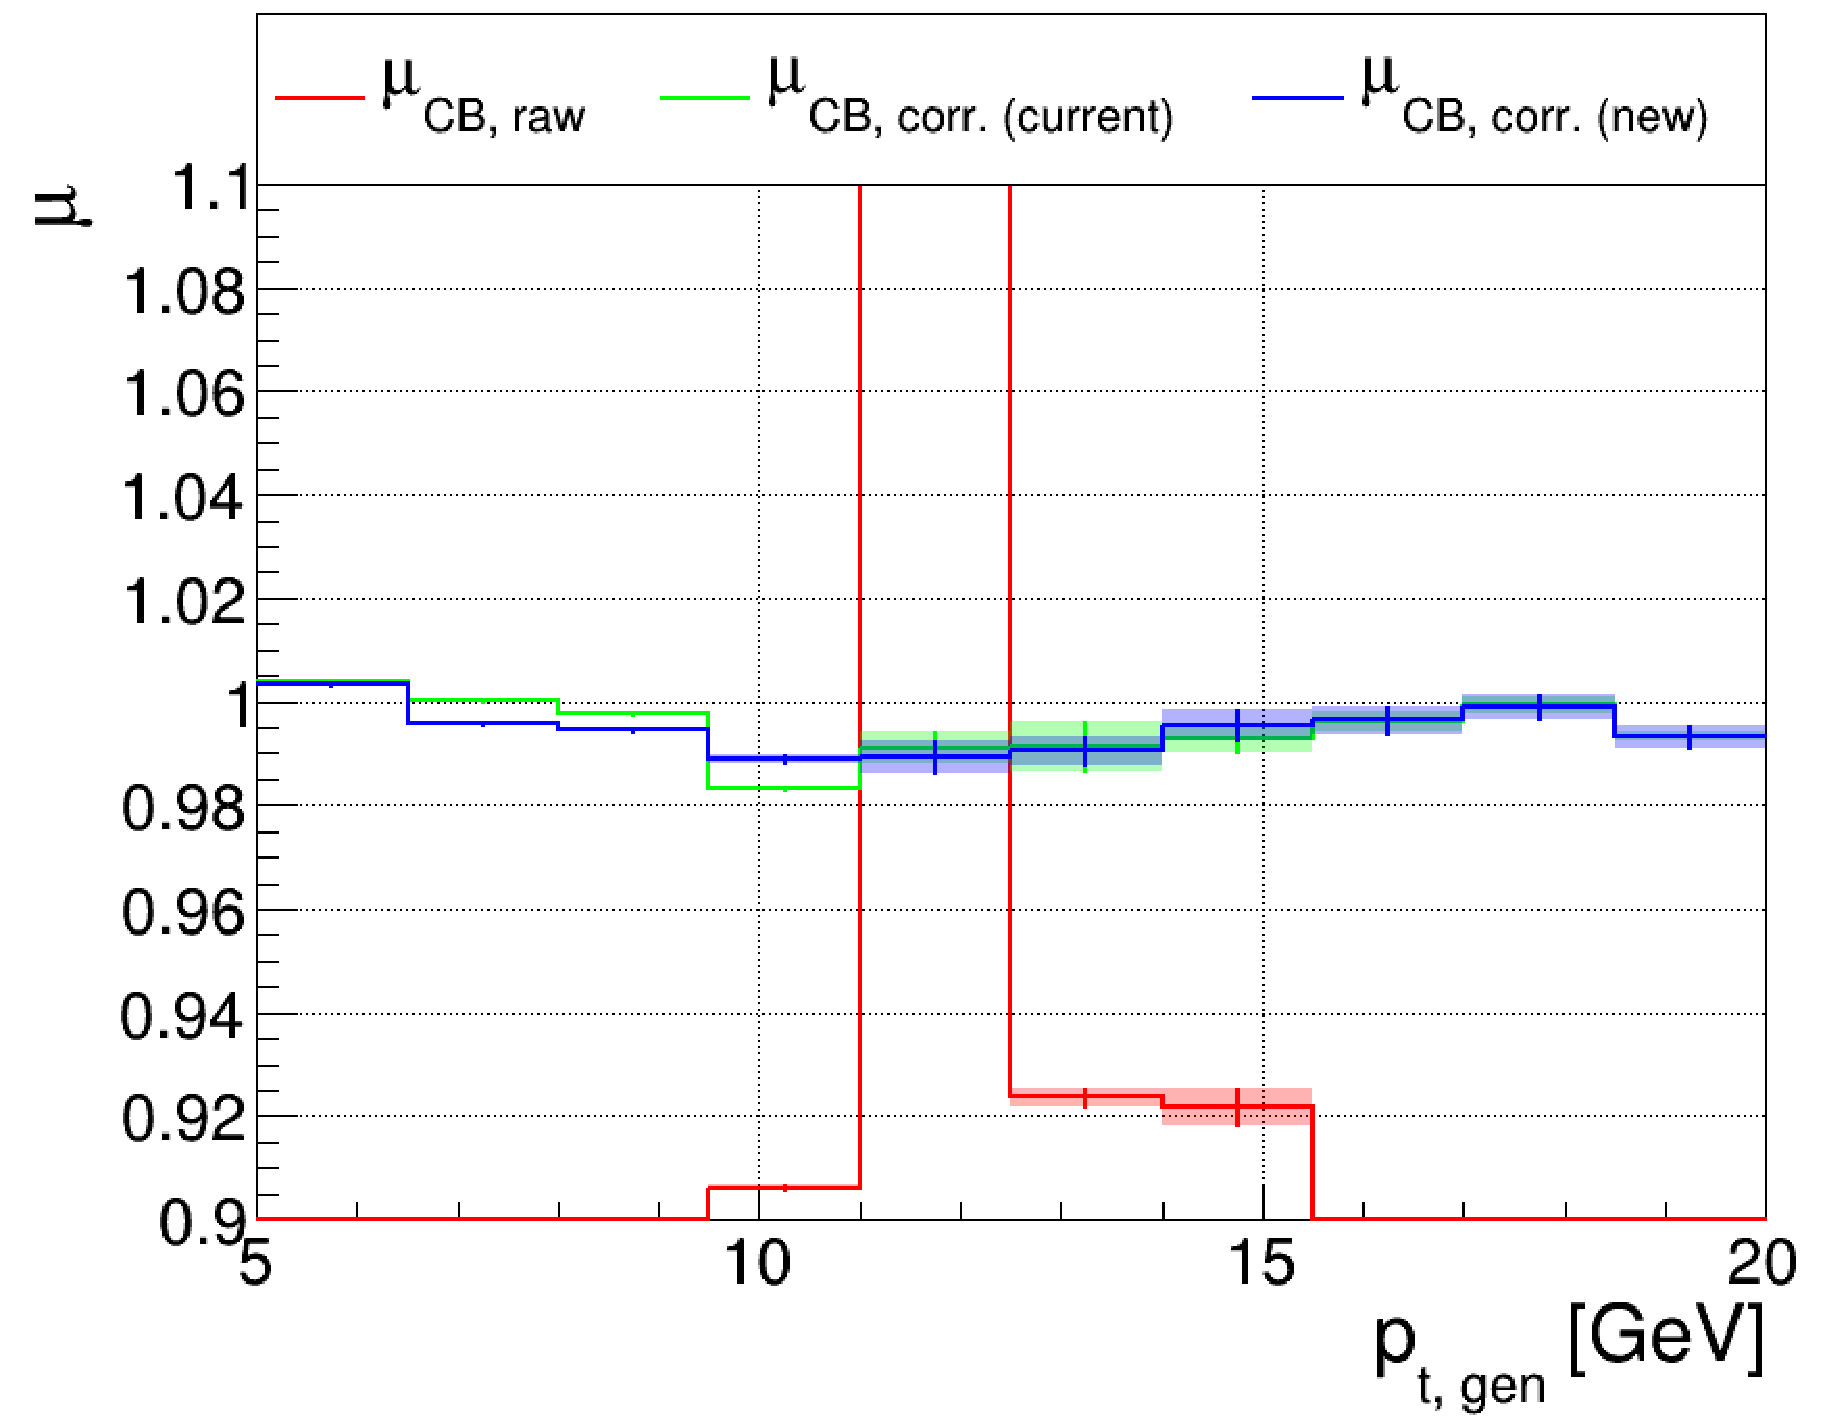
\includegraphics[width=0.495\textwidth]{./ECAL_plots/plotsNoPU/EE/pdf/FULL/GENPT/EEFULL_GENPT_0005_0020_MuOverBins.pdf}
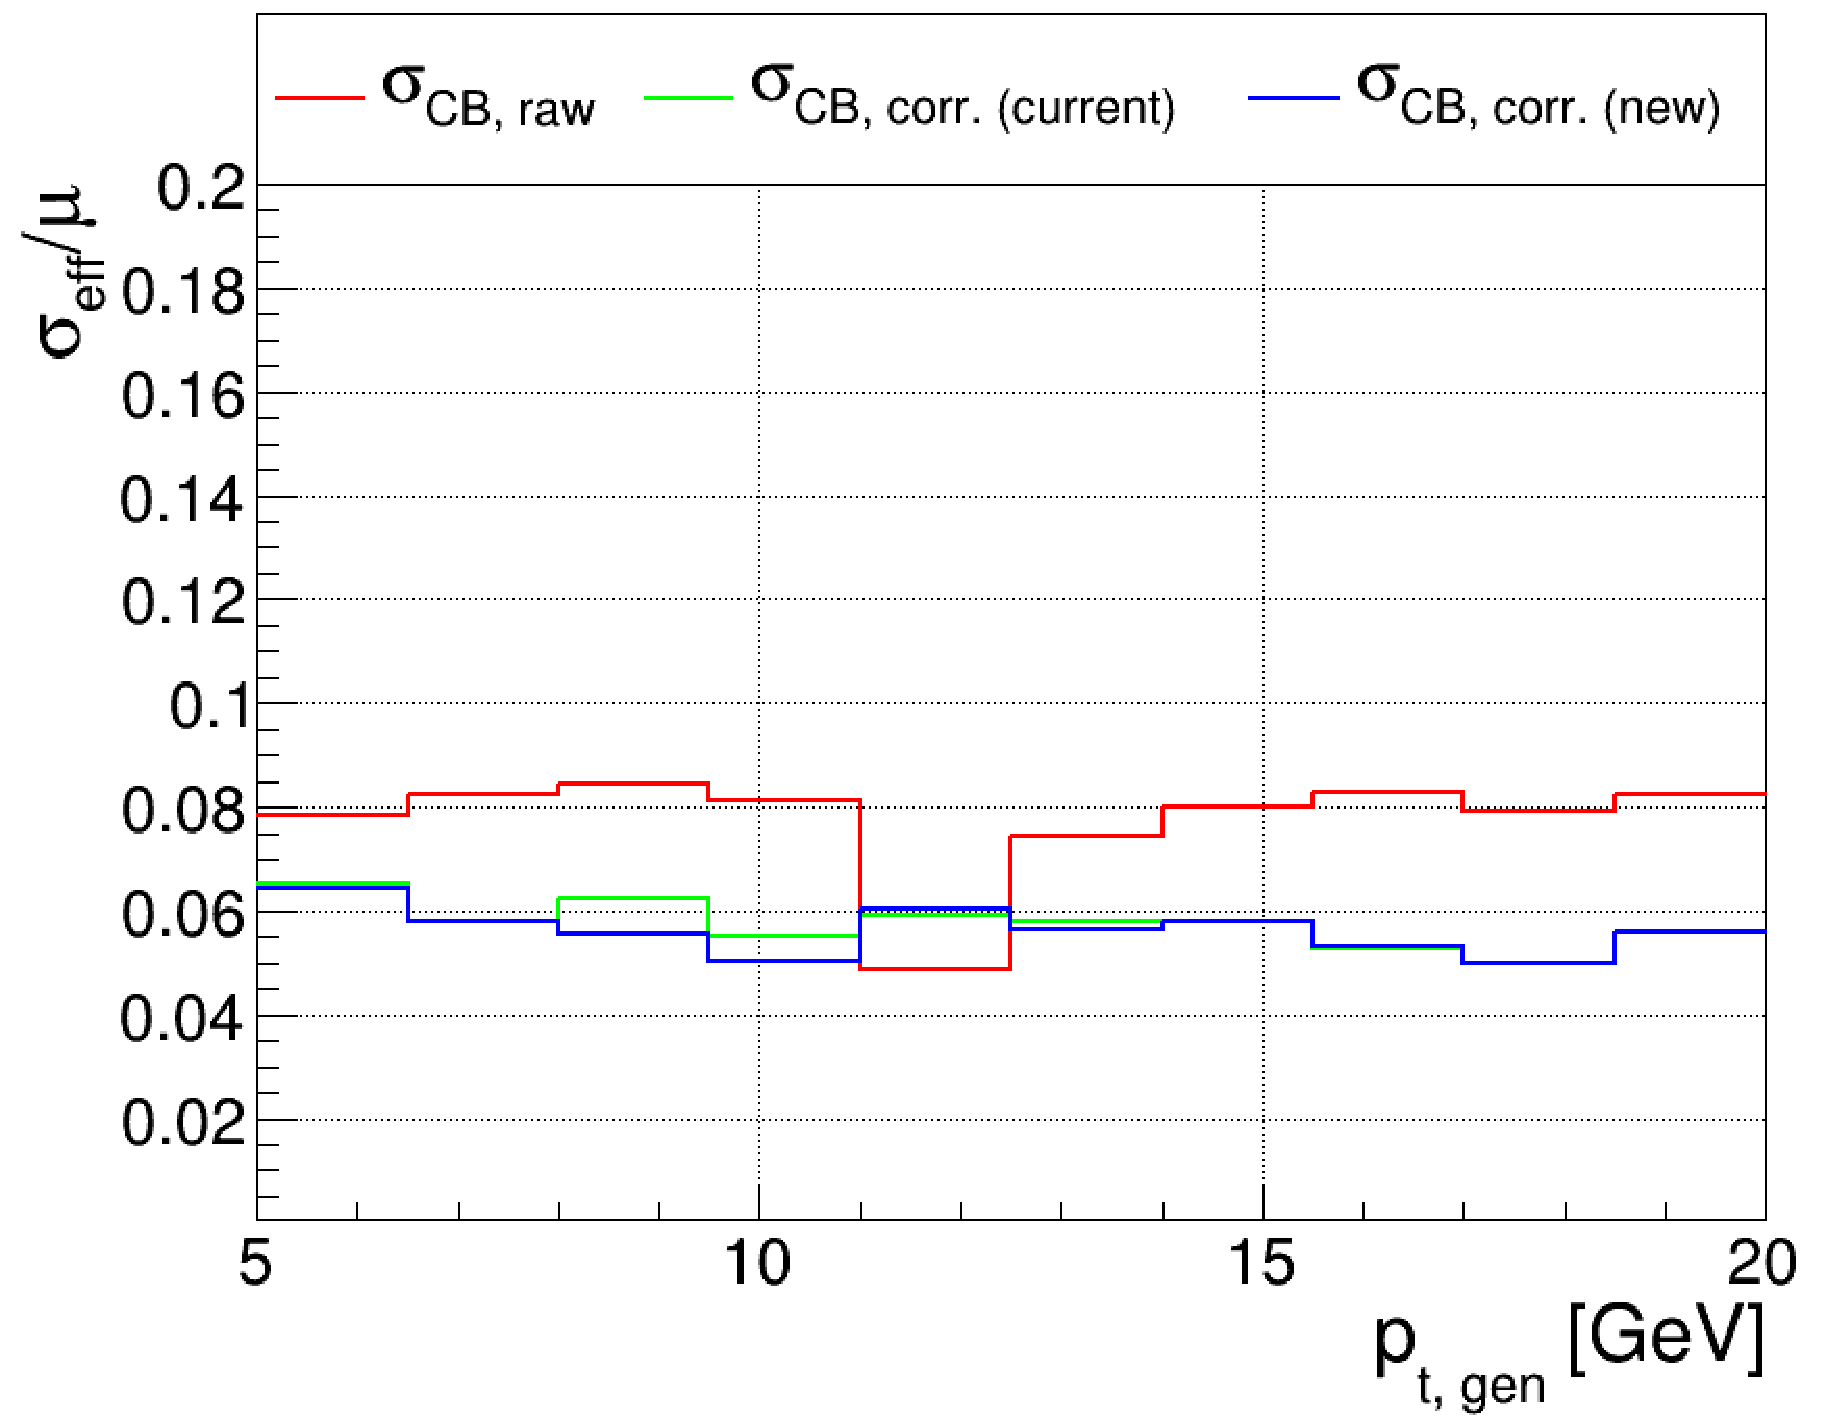
\includegraphics[width=0.495\textwidth]{./ECAL_plots/plotsNoPU/EE/pdf/FULL/GENPT/EEFULL_GENPT_0005_0020_EffSigmaOverBins.pdf}
%\caption{EE - Full Readout pt 5-20}
%\end{figure}
%\begin{figure}
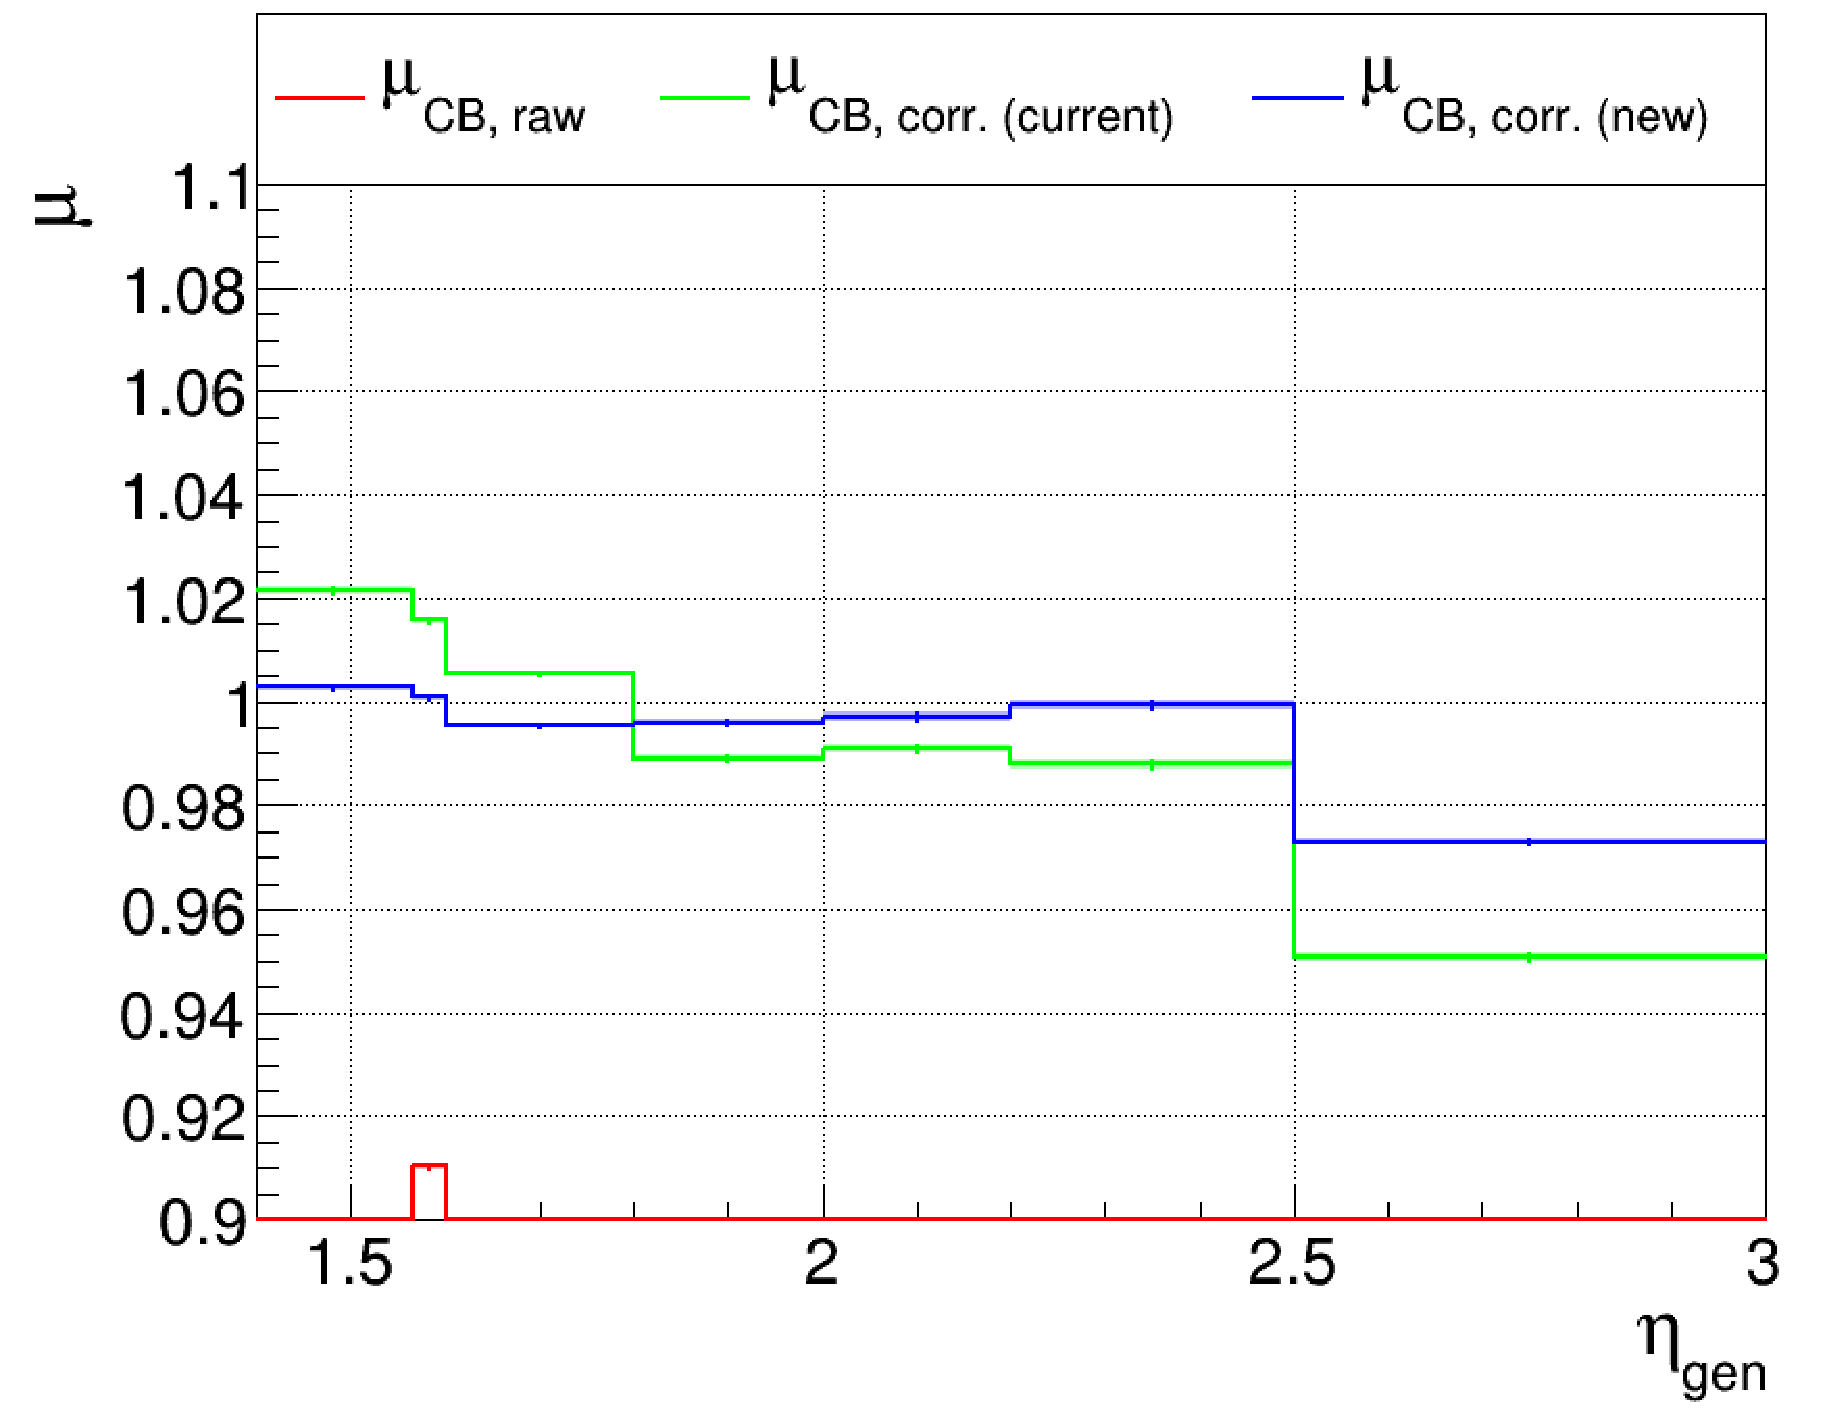
\includegraphics[width=0.495\textwidth]{./ECAL_plots/plotsNoPU/EE/pdf/FULL/GENETA/EEFULL_GENETA_0005_0020_MuOverBins.pdf}
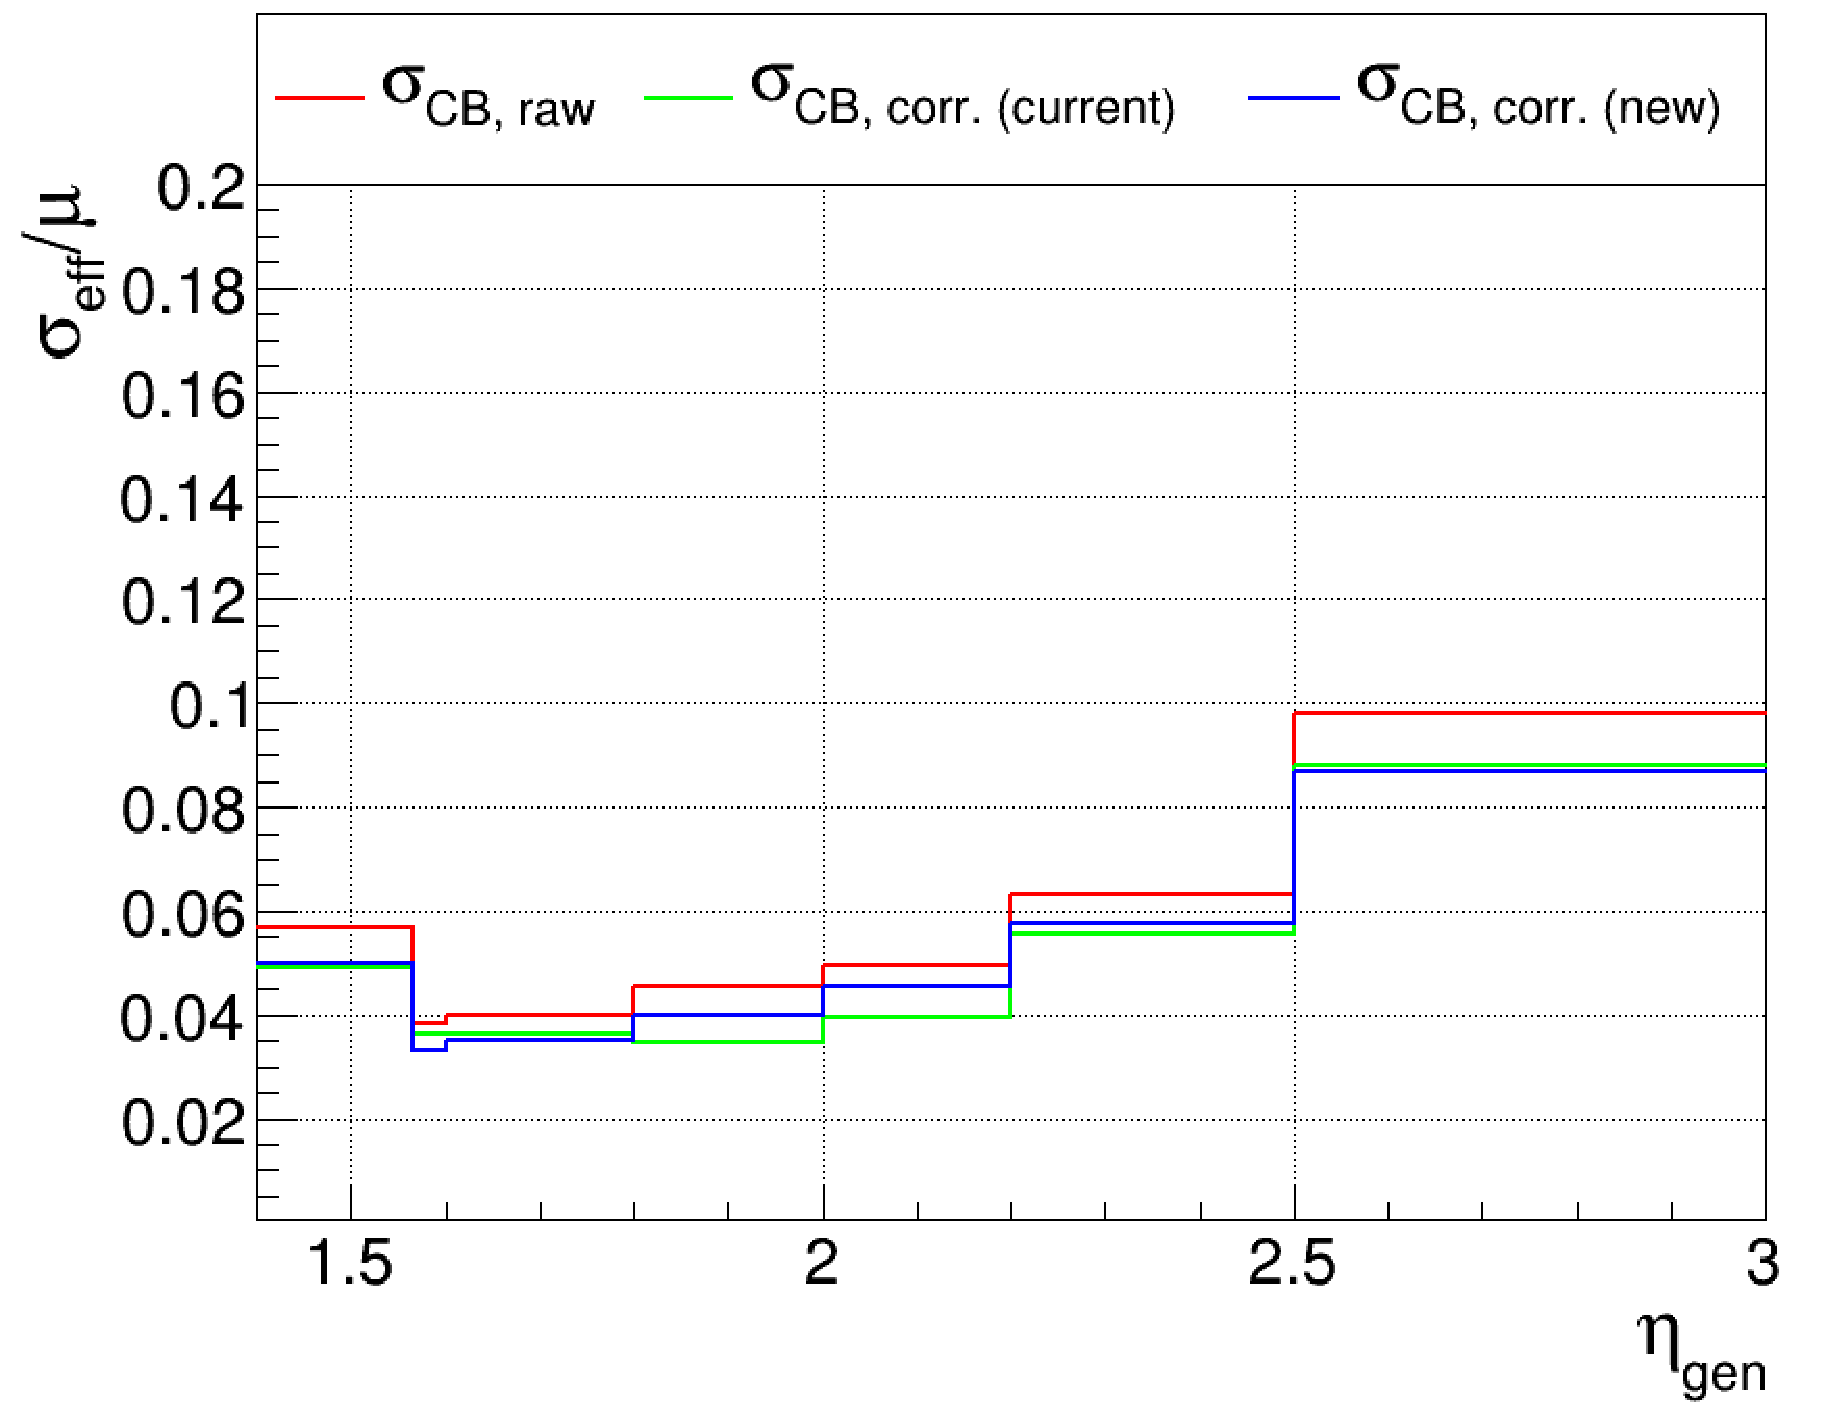
\includegraphics[width=0.495\textwidth]{./ECAL_plots/plotsNoPU/EE/pdf/FULL/GENETA/EEFULL_GENETA_0005_0020_EffSigmaOverBins.pdf}
\caption{EE - Full Readout pt 5-20}
\end{figure}


\begin{figure}
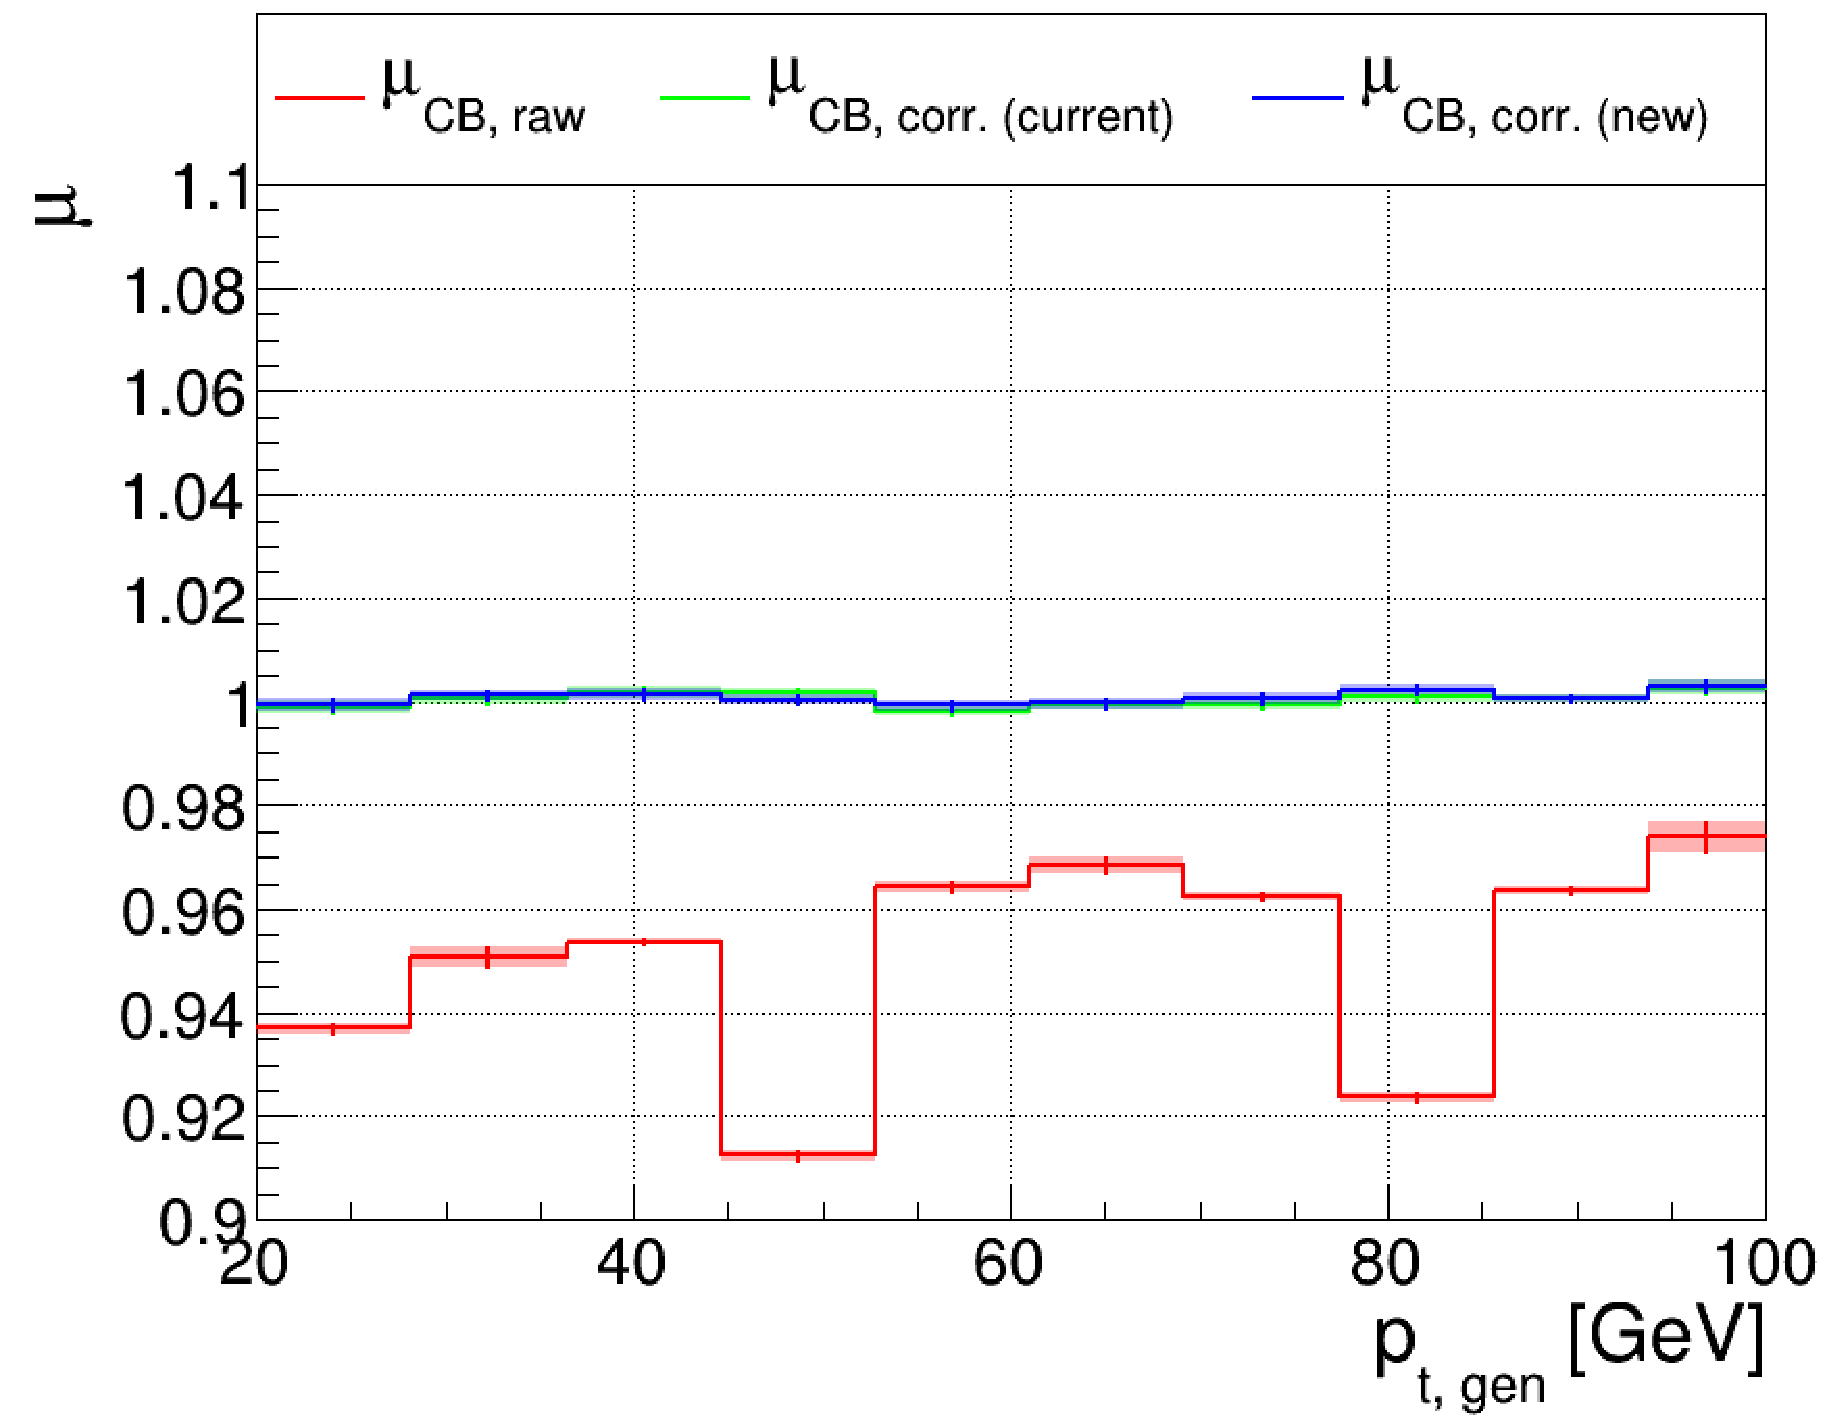
\includegraphics[width=0.495\textwidth]{./ECAL_plots/plotsNoPU/EE/pdf/FULL/GENPT/EEFULL_GENPT_0020_0100_MuOverBins.pdf}
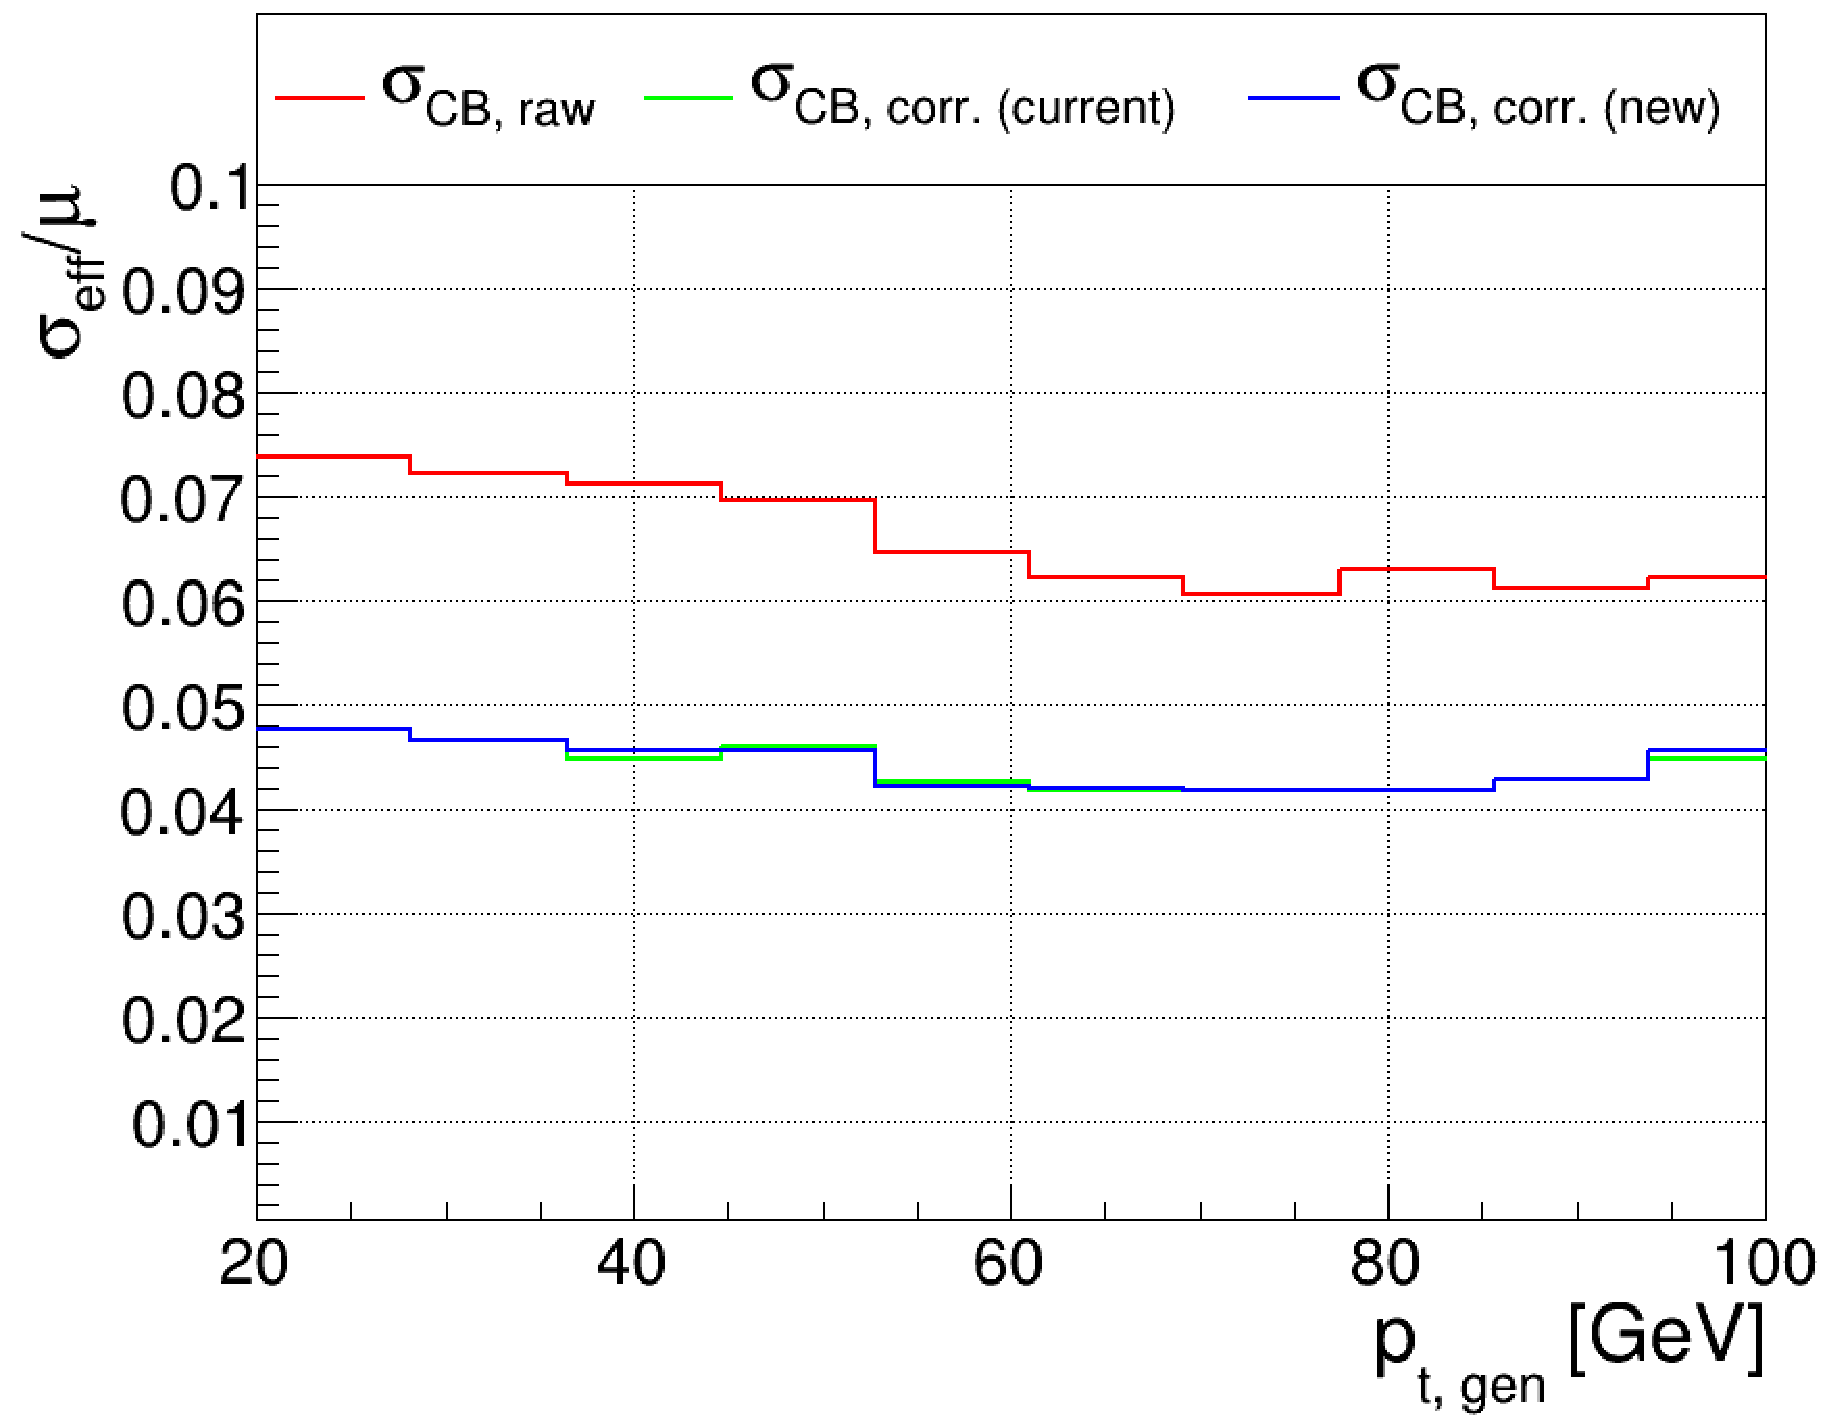
\includegraphics[width=0.495\textwidth]{./ECAL_plots/plotsNoPU/EE/pdf/FULL/GENPT/EEFULL_GENPT_0020_0100_EffSigmaOverBins.pdf}
%\caption{EE - Full Readout pt 20-100}
%\end{figure}
%\begin{figure}
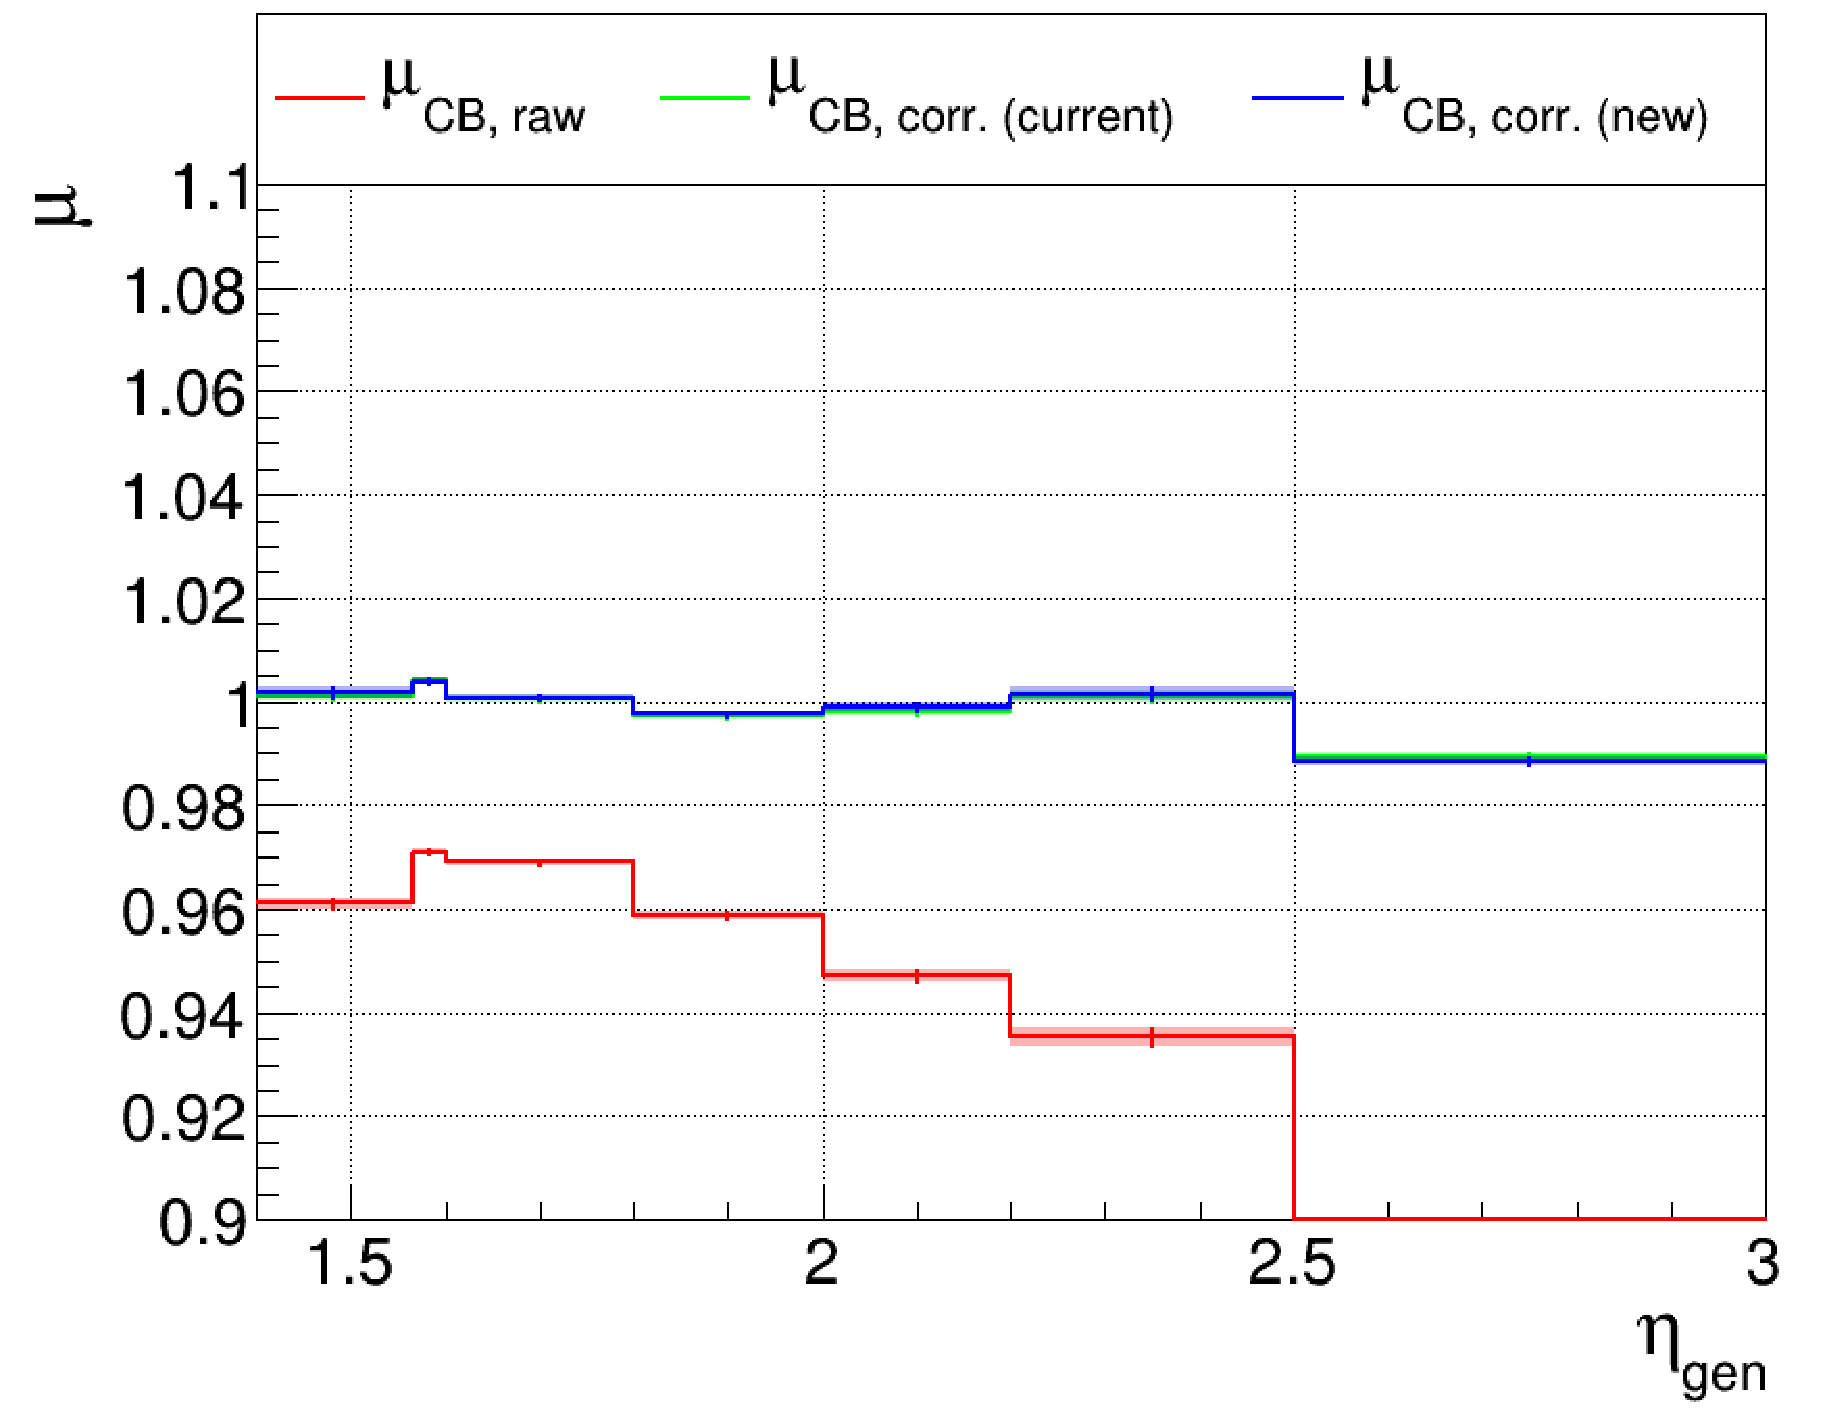
\includegraphics[width=0.495\textwidth]{./ECAL_plots/plotsNoPU/EE/pdf/FULL/GENETA/EEFULL_GENETA_0020_0100_MuOverBins.pdf}
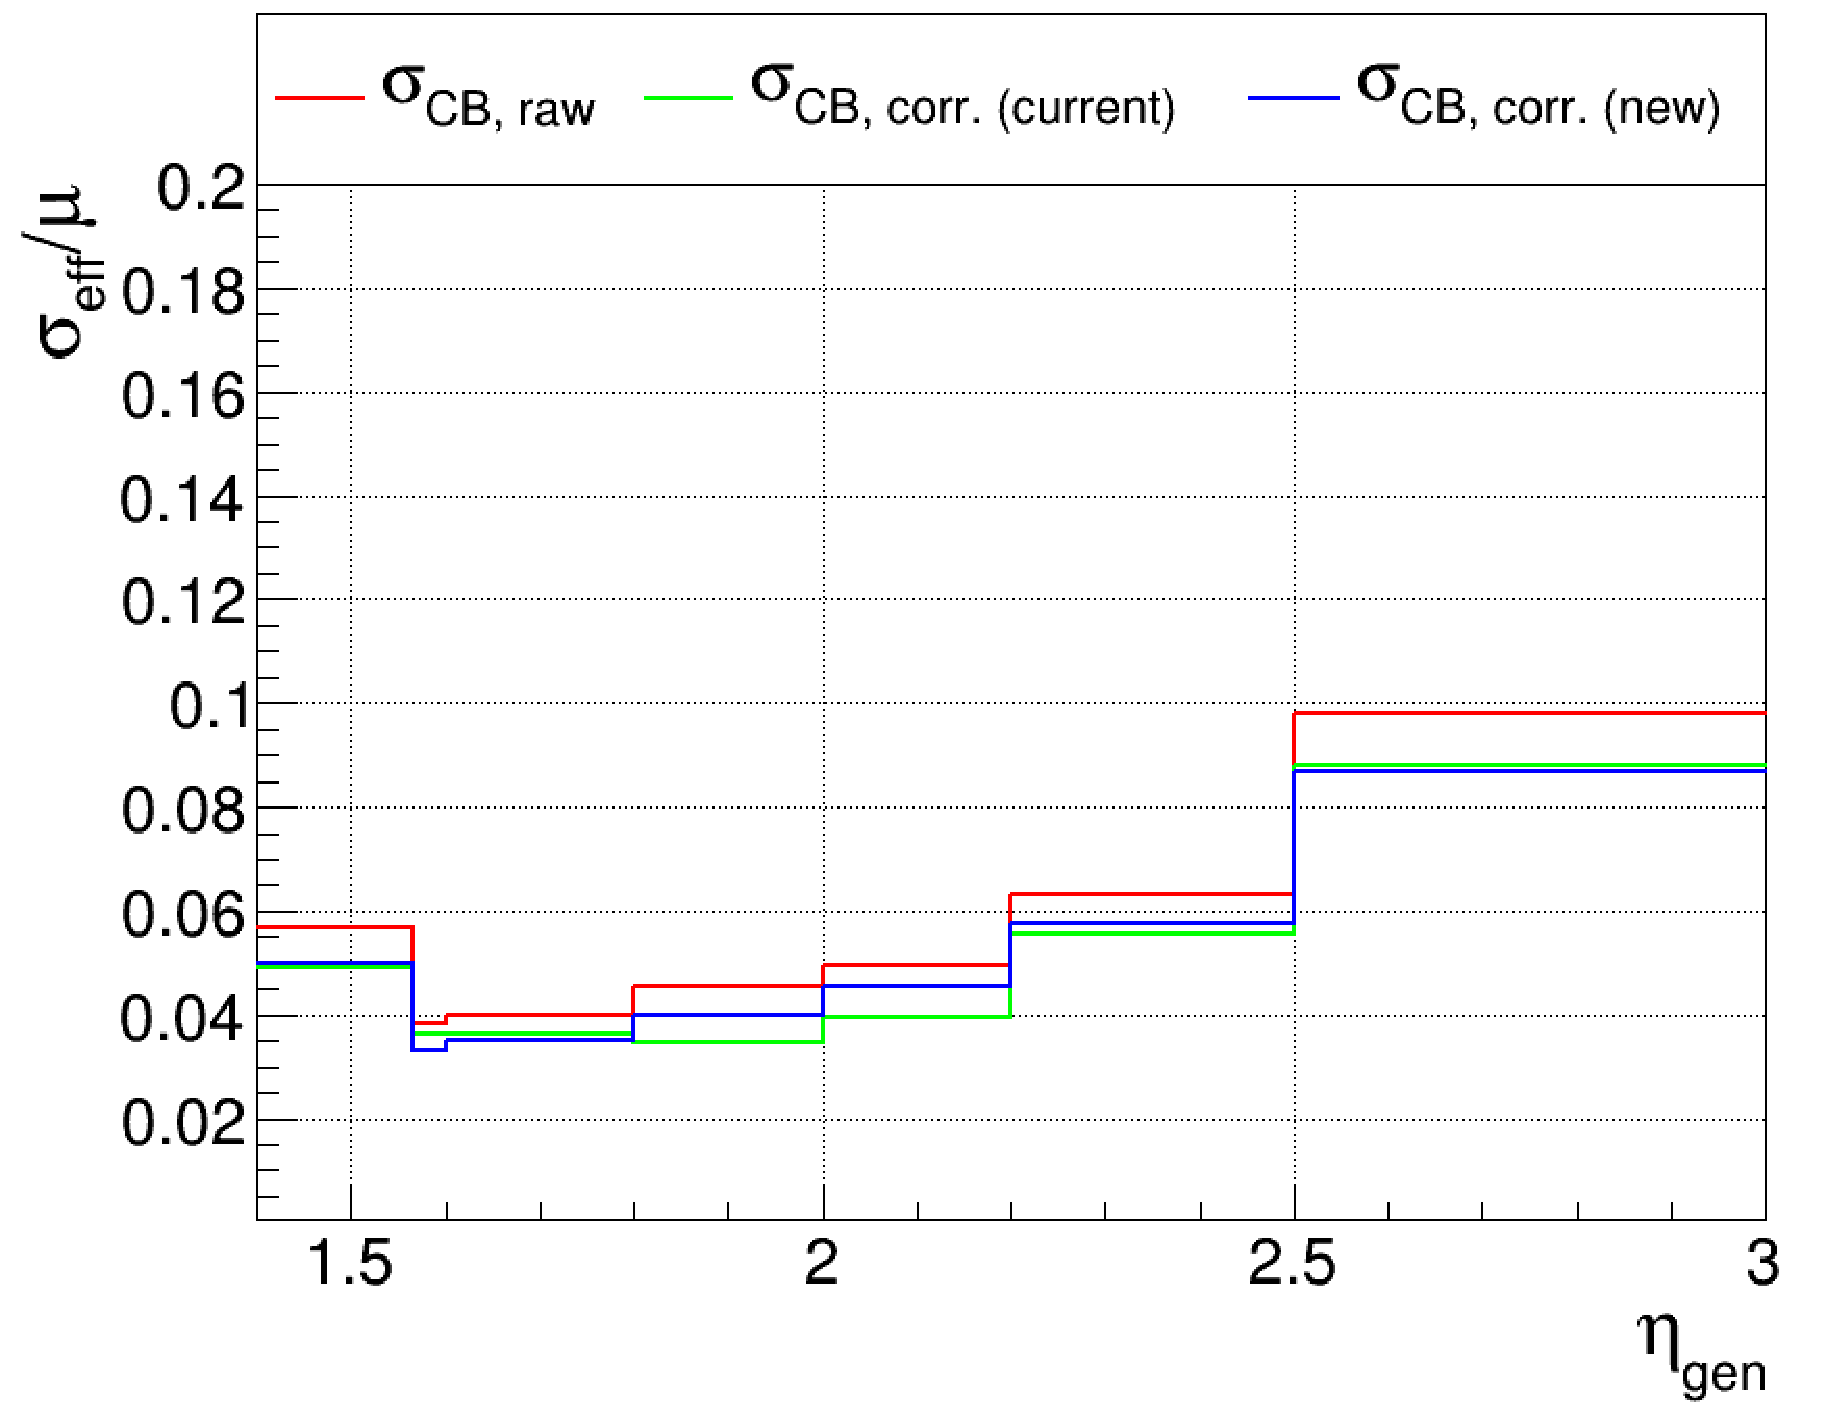
\includegraphics[width=0.495\textwidth]{./ECAL_plots/plotsNoPU/EE/pdf/FULL/GENETA/EEFULL_GENETA_0005_0020_EffSigmaOverBins.pdf}
\caption{EE - Full Readout pt 20-100}
\end{figure}


\begin{figure}
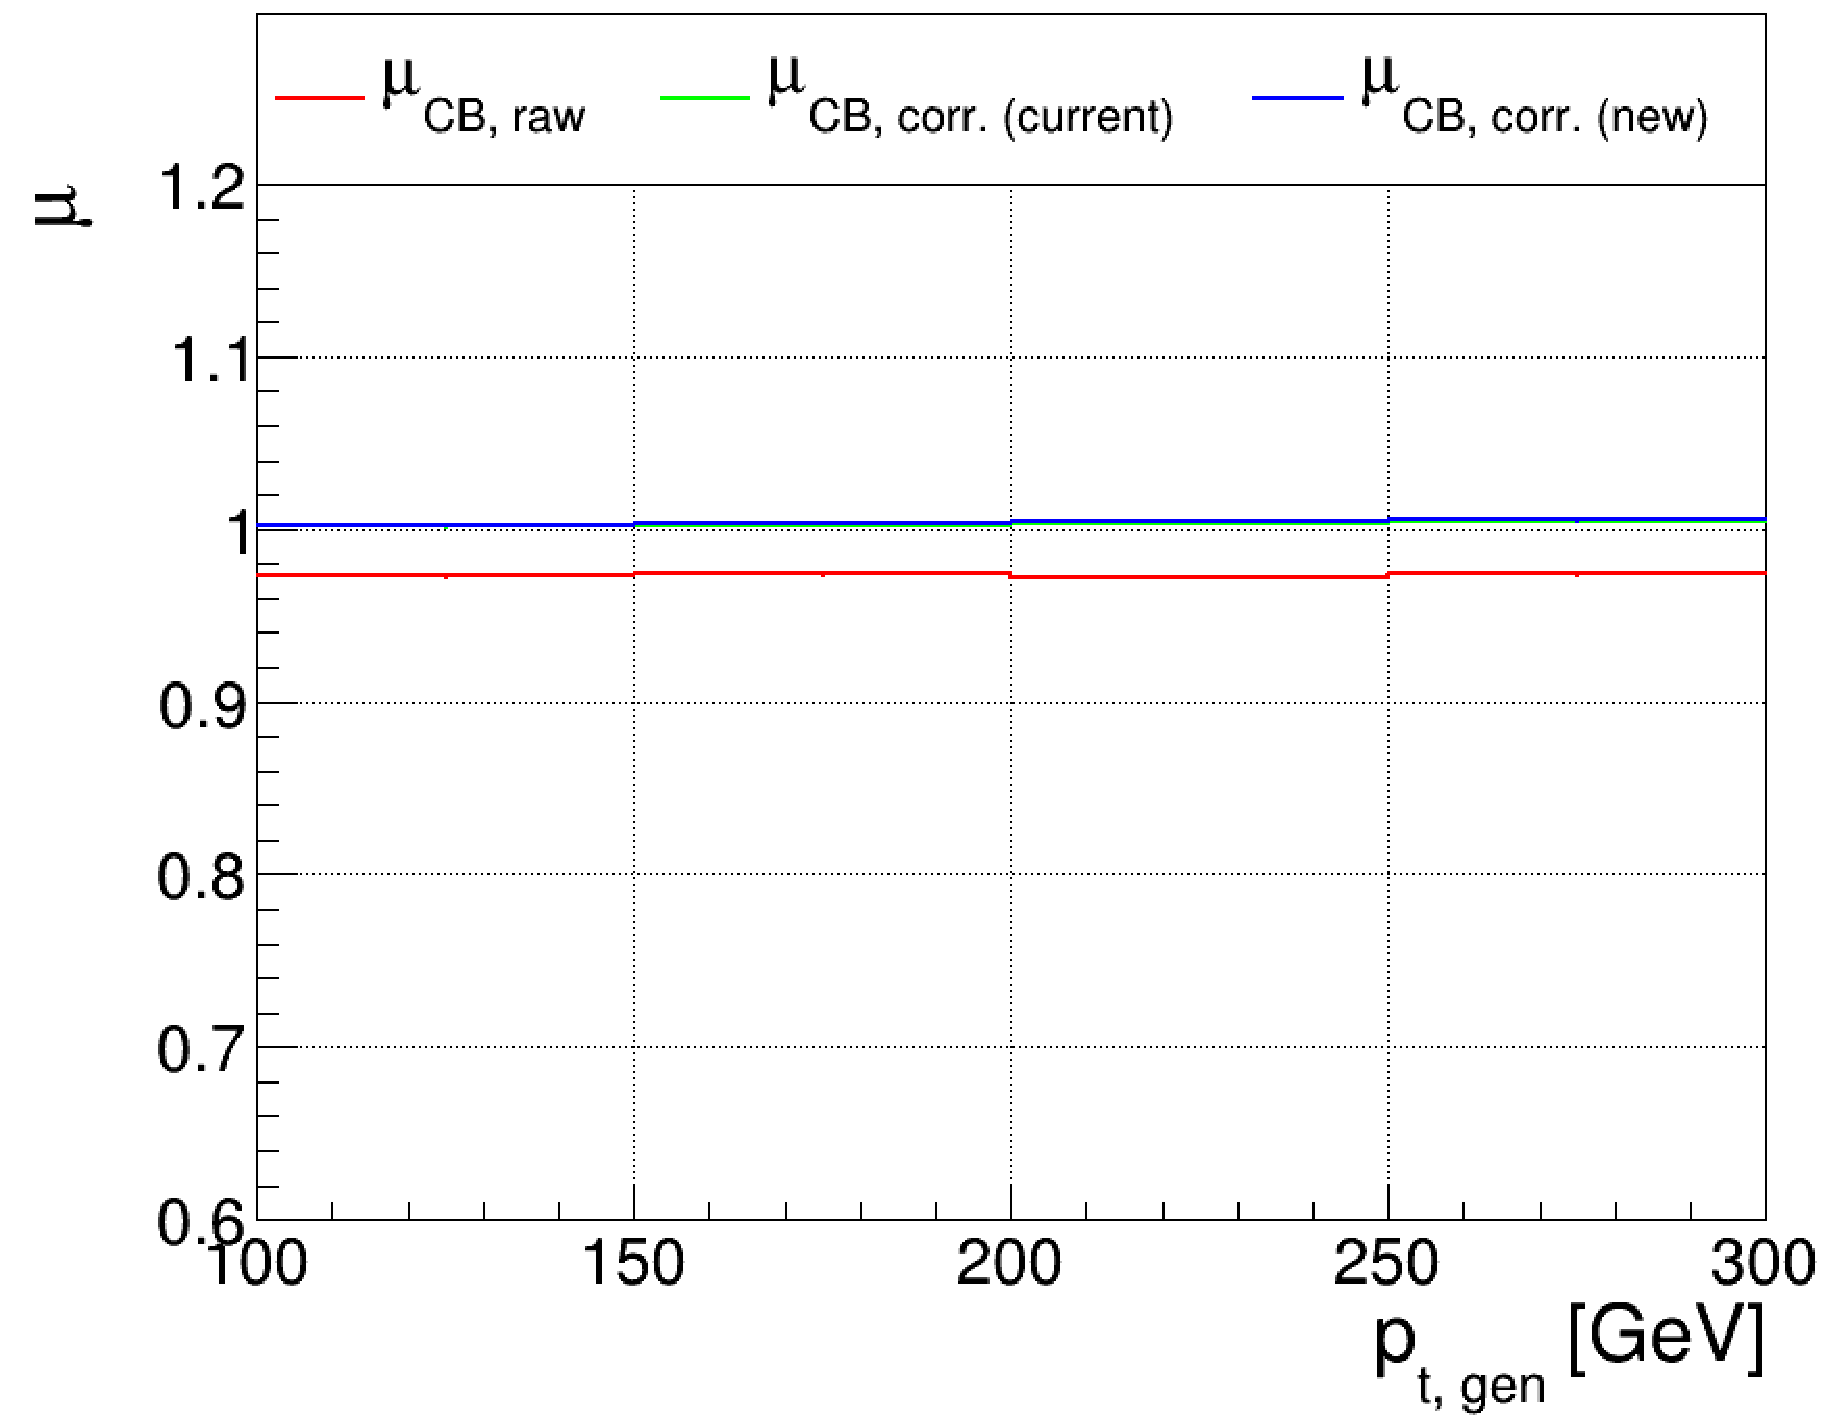
\includegraphics[width=0.495\textwidth]{./ECAL_plots/plotsNoPU/EE/pdf/FULL/GENPT/EEFULL_GENPT_0100_0300_MuOverBins.pdf}
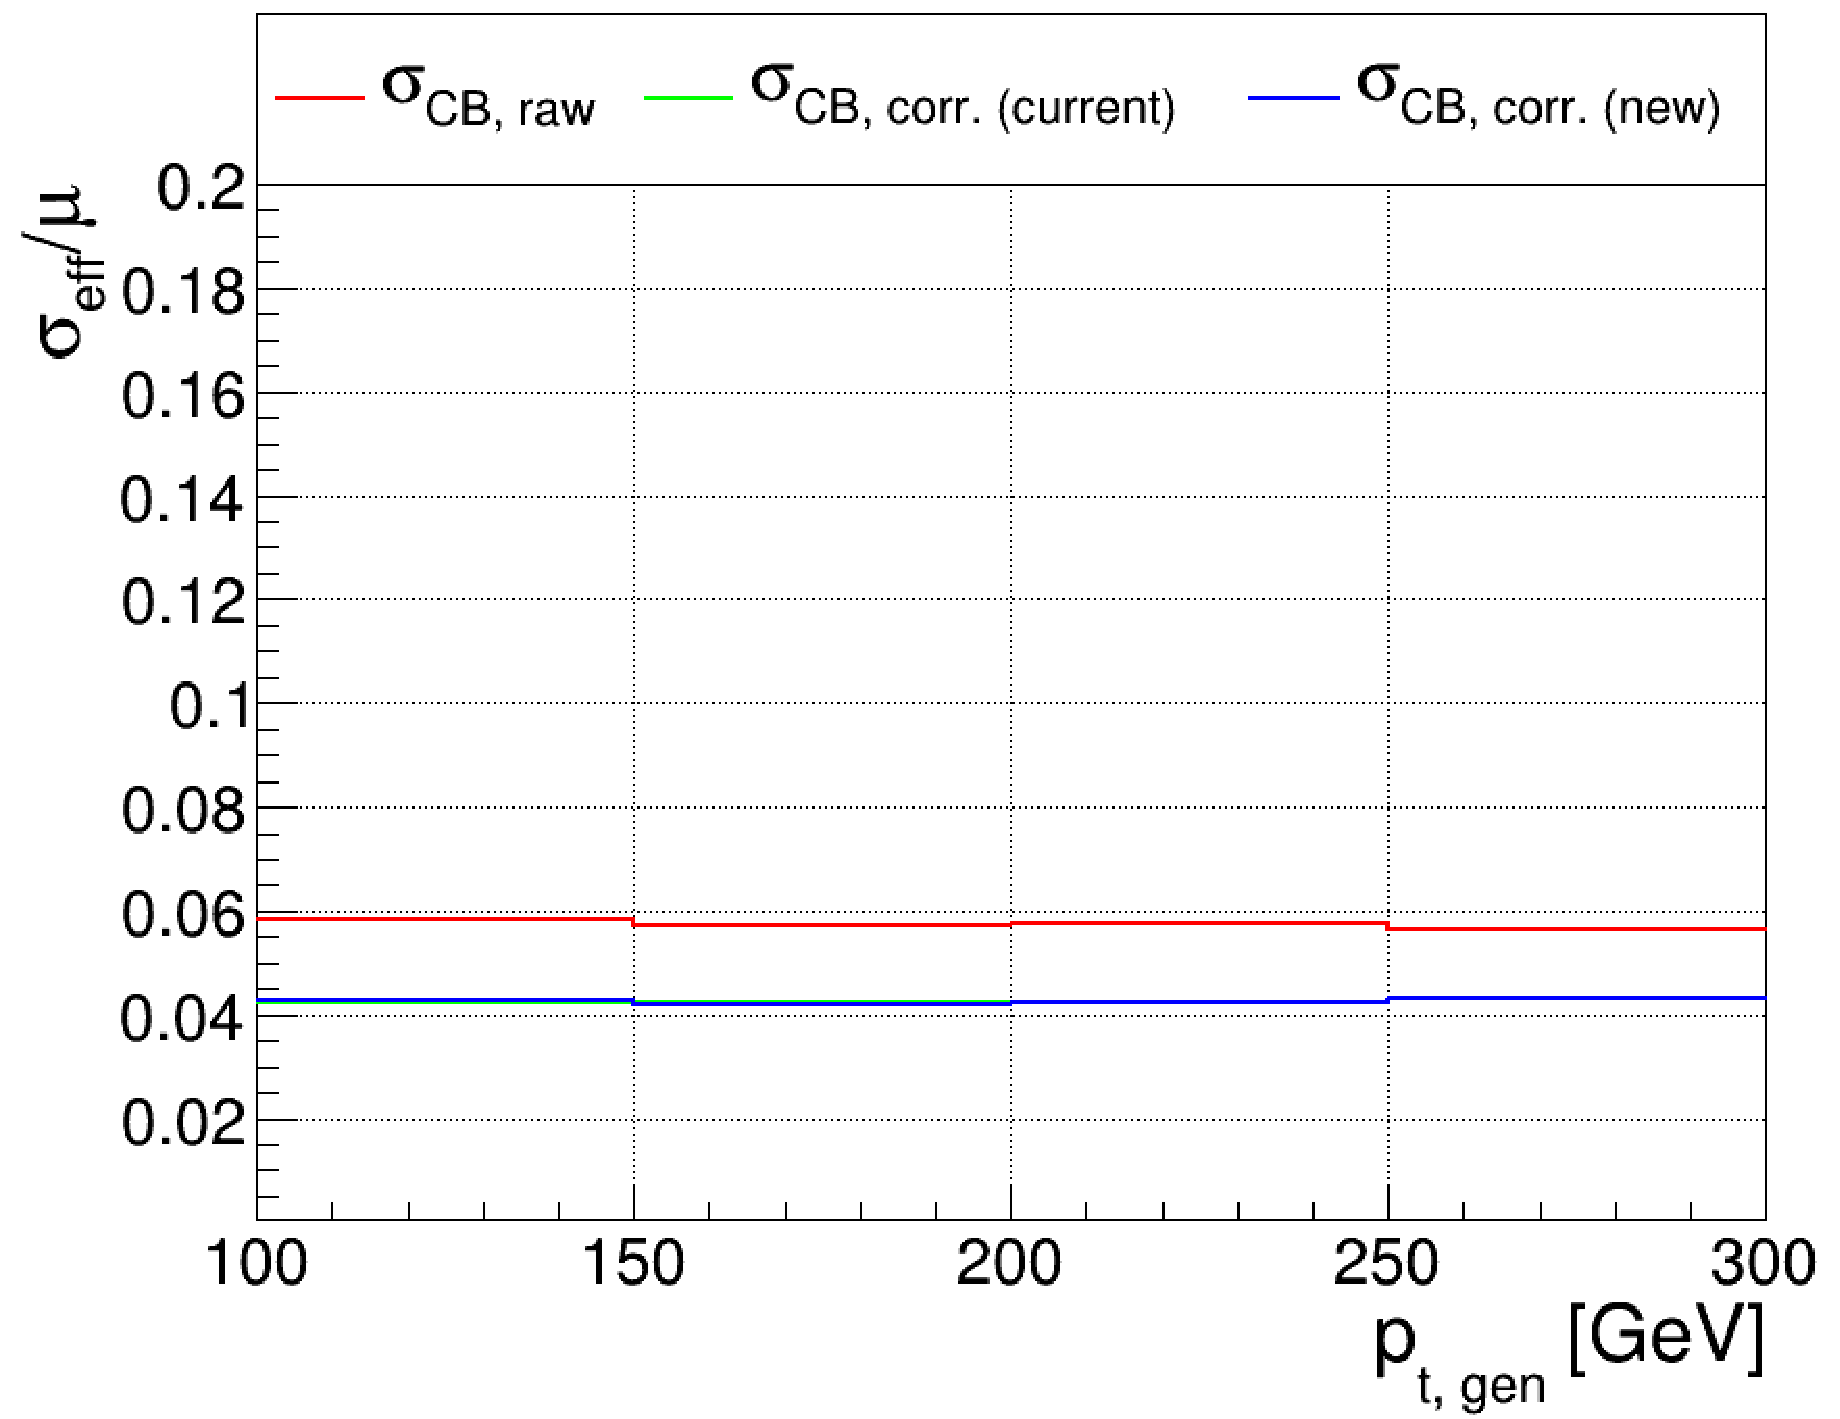
\includegraphics[width=0.495\textwidth]{./ECAL_plots/plotsNoPU/EE/pdf/FULL/GENPT/EEFULL_GENPT_0100_0300_EffSigmaOverBins.pdf}
%\caption{EE - Full Readout pt 100-300}
%\end{figure}
%\begin{figure}
\includegraphics[width=0.495\textwidth]{./ECAL_plots/plotsNoPU/EE/pdf/FULL/GENETA/EEFULL_GENETA_0100_0300_MuOverBins.pdf}
\includegraphics[width=0.495\textwidth]{./ECAL_plots/plotsNoPU/EE/pdf/FULL/GENETA/EEFULL_GENETA_0005_0020_EffSigmaOverBins.pdf}
\caption{EE - Full Readout pt 100-300}
\end{figure}





\begin{figure}
\includegraphics[width=0.495\textwidth]{./plots_pdf/ECAL_plots/plotsNoPU/EE/pdf/ZS/GENPT/EEZS_GENPT_0000_0006_MuOverBins.pdf}
\includegraphics[width=0.495\textwidth]{./plots_pdf/ECAL_plots/plotsNoPU/EE/pdf/ZS/GENPT/EEZS_GENPT_0000_0006_EffSigmaOverBins.pdf}

\includegraphics[width=0.495\textwidth]{./plots_pdf/ECAL_plots/plotsNoPU/EE/pdf/ZS/GENETA/EEZS_GENETA_0000_0006_MuOverBins.pdf}
\includegraphics[width=0.495\textwidth]{./plots_pdf/ECAL_plots/plotsNoPU/EE/pdf/ZS/GENETA/EEZS_GENETA_0000_0006_EffSigmaOverBins.pdf}
\caption[$\mu$ ($\sigma_\mathrm{eff}$) vs \pt of PF ECAL cluster - EE ZS readout NoPU scenario]{Mean response (resolution) defined by Raw PF ECAL clusters (red), the calibration derived earlier in Ru\
n3 based on 126X (green), and the new correction from 2024 simulation sample based on 133X (blue).\pt 0--6\GeV in EE region ZS Readout NOPU scenario.}
\end{figure}

%% %\begin{figure}
%% \includegraphics[width=0.495\textwidth]{./plots_pdf/ECAL_plots/plotsNoPU/EE/pdf/ZS/GENPT/EEZS_GENPT_0006_0025_MuOverBins.pdf}
%% \includegraphics[width=0.495\textwidth]{./plots_pdf/ECAL_plots/plotsNoPU/EE/pdf/ZS/GENPT/EEZS_GENPT_0006_0025_EffSigmaOverBins.pdf}
%% %\caption{EE - ZS Readout pt 6-25}
%% %\end{figure}
%% %\begin{figure}
%% \includegraphics[width=0.495\textwidth]{./plots_pdf/ECAL_plots/plotsNoPU/EE/pdf/ZS/GENETA/EEZS_GENETA_0006_0025_MuOverBins.pdf}
%% %\includegraphics[width=0.495\textwidth]{./ECAL_plots/plotsNoPU/EE/pdf/ZS/GENETA/EEZS_GENETA_0006_0025_EffSigmaOverBins.pdf}
%% \caption{EE - ZS Readout \pt 6-25}
%% \end{figure}




\begin{figure}
\includegraphics[width=0.495\textwidth]{./plots_pdf/ECAL_plots/plotsPU/EE/FULL/pdf/GENPT/EEFULL_GENPT_0005_0020_MuOverBins.pdf}
\includegraphics[width=0.495\textwidth]{./plots_pdf/ECAL_plots/plotsPU/EE/FULL/pdf/GENPT/EEFULL_GENPT_0005_0020_EffSigmaOverBins.pdf}
\includegraphics[width=0.495\textwidth]{./plots_pdf/ECAL_plots/plotsPU/EE/FULL/pdf/GENPT/EEFULL_GENPT_0020_0100_MuOverBins.pdf}
\includegraphics[width=0.495\textwidth]{./plots_pdf/ECAL_plots/plotsPU/EE/FULL/pdf/GENPT/EEFULL_GENPT_0020_0100_EffSigmaOverBins.pdf}
\includegraphics[width=0.495\textwidth]{./plots_pdf/ECAL_plots/plotsPU/EE/FULL/pdf/GENPT/EEFULL_GENPT_0100_0300_MuOverBins.pdf}
\includegraphics[width=0.495\textwidth]{./plots_pdf/ECAL_plots/plotsPU/EE/FULL/pdf/GENPT/EEFULL_GENPT_0100_0300_EffSigmaOverBins.pdf}

\caption [$\mu$ ($\sigma_\mathrm{eff}$) vs \pt of PF ECAL cluster - EE full readout PU scenario]{Mean response (resolution) defined by Raw PF ECAL clusters (red), the calibration derived earlier in Ru\
n3 based on 126X (green), and the new correction from 2024 simulation sample based on 133X (blue). (top) low \pt, (middle) mid \pt, (bottom) high \pt in EE region full readout PU scenario.}
\label{fig:PU_EEFULL_pt}
\end{figure}


\begin{figure}
\includegraphics[width=0.495\textwidth]{./plots_pdf/ECAL_plots/plotsPU/EE/FULL/pdf/GENETA/EEFULL_GENETA_0005_0020_MuOverBins.pdf}
\includegraphics[width=0.495\textwidth]{./plots_pdf/ECAL_plots/plotsPU/EE/FULL/pdf/GENETA/EEFULL_GENETA_0005_0020_EffSigmaOverBins.pdf}
\includegraphics[width=0.495\textwidth]{./plots_pdf/ECAL_plots/plotsPU/EE/FULL/pdf/GENETA/EEFULL_GENETA_0020_0100_MuOverBins.pdf}
\includegraphics[width=0.495\textwidth]{./plots_pdf/ECAL_plots/plotsPU/EE/FULL/pdf/GENETA/EEFULL_GENETA_0020_0100_EffSigmaOverBins.pdf}
\includegraphics[width=0.495\textwidth]{./plots_pdf/ECAL_plots/plotsPU/EE/FULL/pdf/GENETA/EEFULL_GENETA_0100_0300_MuOverBins.pdf}
\includegraphics[width=0.495\textwidth]{./plots_pdf/ECAL_plots/plotsPU/EE/FULL/pdf/GENETA/EEFULL_GENETA_0100_0300_EffSigmaOverBins.pdf}


\caption [$\mu$ ($\sigma_\mathrm{eff}$) vs $\eta$ of PF ECAL cluster - EE Full readout PU scenario]{Mean response (resolution) defined by Raw PF ECAL clusters (red), the calibration derived earlier in\
 Run3 based on 126X (green), and the new correction from 2024 simulation sample based on 133X (blue). (top) low $\eta$, (middle) mid $\eta$, (bottom) high $\eta$ in EE region Full readout PU scenario.}
\label{fig:PU_EEFULL_eta}
\end{figure}

\begin{figure}
\includegraphics[width=0.495\textwidth]{./plots_pdf/ECAL_plots/plotsPU/EE/ZS/pdf/GENPT/EEZS_GENPT_0000_0006_MuOverBins.pdf}
\includegraphics[width=0.495\textwidth]{./plots_pdf/ECAL_plots/plotsPU/EE/ZS/pdf/GENPT/EEZS_GENPT_0000_0006_EffSigmaOverBins.pdf}

\includegraphics[width=0.495\textwidth]{./plots_pdf/ECAL_plots/plotsPU/EE/ZS/pdf/GENETA/EEZS_GENETA_0000_0006_MuOverBins.pdf}
\includegraphics[width=0.495\textwidth]{./plots_pdf/ECAL_plots/plotsPU/EE/ZS/pdf/GENETA/EEZS_GENETA_0000_0006_EffSigmaOverBins.pdf}

\caption[$\mu$ ($\sigma_\mathrm{eff}$) vs. \pt of PF ECAL cluster - EE ZS readout PU scenario]{Mean response (resolution) defined by raw PF ECAL clusters (red), the calibration derived earlier in Run~3 based on 126X (green), and the new correction from the 2024 simulation sample based on 133X (blue).\pt 0--6\GeV in EE region ZS readout PU scenario.}
\label{fig:PU_EEZS}
\end{figure}

%% %\begin{figure}
%% \includegraphics[width=0.495\textwidth]{./plots_pdf/ECAL_plots/plotsPU/EE/ZS/pdf/GENPT/EEZS_GENPT_0006_0025_MuOverBins.pdf}
%% \includegraphics[width=0.495\textwidth]{./plots_pdf/ECAL_plots/plotsPU/EE/ZS/pdf/GENPT/EEZS_GENPT_0006_0025_EffSigmaOverBins.pdf}
%% %\caption{EE - ZS Readout pt 6-25}
%% %\end{figure}
%% %\begin{figure}
%% \includegraphics[width=0.495\textwidth]{./plots_pdf/ECAL_plots/plotsPU/EE/ZS/pdf/GENETA/EEZS_GENETA_0006_0025_MuOverBins.pdf}
%% \caption{EE - ZS Readout \pt 6-25}
%% \end{figure}










HLT vs offline PF ECAL cluster
first for NoPU samples




%%%%%%%%%%%%%%%%%%%%%%%%%%%%%%%%%%%%%%%%%%%%%%%                                                                                                                                     
\begin{figure}
\includegraphics[width=0.495\textwidth]{./ECAL_plots/Prod6/NoPU/H_GenPi_Pt_vs_RespE.pdf}
%\caption{(PF cluster offline E / PFC online E) vs pt}
\includegraphics[width=0.495\textwidth]{./ECAL_plots/Prod6/NoPU/H_GenPi_Eta_vs_RespE.pdf}
\caption{(PF cluster offline E / PFC online E)}
\end{figure}

\begin{figure}
\includegraphics[width=0.495\textwidth]{./ECAL_plots/Prod6/NoPU/H_GenPi_Pt_vs_RespCE.pdf}
%\caption{(PF cluster offline E corrected / PFC online E corrected) vs pt}
\includegraphics[width=0.495\textwidth]{./ECAL_plots/Prod6/NoPU/H_GenPi_Eta_vs_RespCE.pdf}
\caption{(PF cluster offline E corrected / PFC online E corrected)}
\end{figure}                                                                                                                                                                       
%%%%%%%%%%%%%%%%%%%%%%%%%%%%%%%%%%%%%%%%%%%%%%%%                                                                                                                                    


Second for PUU samples
\begin{figure}
\includegraphics[width=0.495\textwidth]{./plots_pdf/ECAL_plots/Prod6/PU/H_GenPi_Pt_vs_RespE.pdf}
%\caption{(PF cluster offline E / PFC online E) vs pt}                                                                 
\includegraphics[width=0.495\textwidth]{./plots_pdf/ECAL_plots/Prod6/PU/H_GenPi_Eta_vs_RespE.pdf}
\caption{(PF cluster offline E / PFC online E)}
\label{fig:PU_ECAL_Offline_vs_Online_E}
\end{figure}

\begin{figure}
\includegraphics[width=0.495\textwidth]{./plots_pdf/ECAL_plots/Prod6/PU/H_GenPi_Pt_vs_RespCE.pdf}
%\caption{(PF cluster offline E corrected / PFC online E corrected) vs pt}                                             
\includegraphics[width=0.495\textwidth]{./plots_pdf/ECAL_plots/Prod6/PU/H_GenPi_Eta_vs_RespCE.pdf}
\caption{(PF cluster offline E corrected / PFC online E corrected)}
\label{fig:PU_ECAL_Offline_vs_Online_CE}
\end{figure}       

%%%%%%%%%%%%%%%%%%%%%%%%%%%%%%%%%%%%%%%%%%%%%%%%
%\section{Citations}
%Here is a citation \cite{fake1}, and here is another \cite{fake2}. Citations are
%nice. Depending on your choice of bibliography, there may be different formats
%you can use. For example, Chicago provides a family of short citation commands.BB
